\documentclass[a4paper,11pt]{report}
\usepackage[utf8]{inputenc}
\usepackage{float}
\usepackage[LAE, T1]{fontenc}
\usepackage{ifthen}
\usepackage{calc}
\usepackage[english, arabic]{babel}

\usepackage{cmap} % Search and copy Arabi PDF files

\usepackage{url}

\usepackage{graphicx}

\usepackage{siunitx}

% use of ams math, fonts and symbols
\usepackage{amsmath}
\usepackage{amsfonts}
\usepackage{amssymb}

\usepackage{color}
\usepackage{everyshi}

% the package setspace allows us to change the \baseline 
%  (the vertical length of a line), it has three commands:
% \doublespacing    : for double spacing
% \onehalfspacing  : for one line and a half spacing
% \singlespacing     : for default one line spacing
\usepackage{setspace}
\doublespacing
%\onehalfspacing
%\singlespacing

\renewcommand{\I}[1]{\if@farsi\FarsiEncoding\else\ArabicEncoding\fi\textLR{#1}}%
\renewcommand{\EI}[1]{\textLR{\FarsiEncoding  \textLR{#1}}}%

\usepackage{fancyhdr}
\usepackage{lastpage} % enable use of Page n Of m
%\usepackage{tocbibind} %add

% like :
% \rfoot{\footnotesize page \thepage\ of \pageref{LastPage}}	% "Page 1 of 2"

\renewcommand \thechapter {\textLR{\arabic{chapter}}}

\renewcommand\theequation
  {\textLR{\thechapter.{\textLR{\arabic{equation}}}}}

%\renewcommand{\chaptermark}[1]{\markboth{#1}{}}
%\renewcommand{\sectionmark}[1] {{\markright{\thesection\ #1}}}
%\markboth{chapter name}{}

\renewcommand{\thepart}{\textLR{\Roman{part}}}

\renewcommand\thesection
  {\textLR{\thechapter.{\textLR{\arabic{section}}}}}

\renewcommand\thesubsection
  {\textLR{\thesection.{\textLR{\arabic{subsection}}}}}

\renewcommand\thesubsubsection
  {\textLR{\thesubsection.{\textLR{\arabic{subsubsection}}}}}

\renewcommand \thepage
    {\textLR{\arabic{page}}}


\renewcommand\addcontentsline[3]{%
\addtocontents{#1}{%
\protect\contentsline{#2}{#3}{\I{\thepage}}}}



% change the enumeration of chapter, section, subsection, ...
\renewcommand{\thepart}{\textLR{\Roman{part}}}
\renewcommand \thechapter {\textLR{\arabic{chapter}}}

\renewcommand\thesection {\textLR{{\textLR{\arabic{section}.\thechapter}}}}
\renewcommand\thesubsection {\textLR{{\textLR{\arabic{subsection}.\thesection}}}}
\renewcommand\thesubsubsection {\textLR{{\textLR{\arabic{subsubsection}.\thesubsection}}}}


\renewcommand \thepage {\textLR{\arabic{page}}}

\renewcommand \chaptername {\textLR{\arabic{الفصل}}}
\renewcommand \bibname{المراجع}

\renewcommand\addcontentsline[3]{%
\addtocontents{#1}{%
\protect\contentsline{#2}{#3}{\I{\thepage}}}}

\newcommand \azcite[1] {\textLR{\cite{#1}}}
\newcommand \citeLR[1] {\textLR{\cite{#1}}}
\newcommand \citeRL[1] {\textRL{\cite{#1}}}

\def \DetailedCalculation       {1}
\def \MidiumDetailedCalculation {2}
\def \NotDetailedCalculation {3}

\newcommand\azmakefigcaption[2]{%
 \vspace{\abovecaptionskip}%
  \sbox\@tempboxa{#1: #2}%
  \idthenelse{\lengthtest{\wd\@tempboxa >\linewidth}}%
	{\noindent #2: #1\par}%
	{\centering
		\makebox[\linewidth][c]{\usebox\@tempboxa\par}
	}%
  \vspace{\belowcaptionskip}%
}

\renewcommand \thefigure
    {\textLR{{\textLR{\arabic{figure}}}.\thechapter}}

\renewcommand \thetable
    {\textLR{{\textLR{\arabic{table}}}.\thechapter}}

\def\fnum@figure{\I{\thefigure}\nobreakspace\figurename}

\newsavebox{\tempboxaz}

\newcommand\azfigcaption[1]{%
  \refstepcounter{figure} 
  \ifx\@captype\@undefined
    \@latex@error{\noexpand\caption outside float}\@ehd
    \expandafter\@gobble%
  \else%
	\ifx\@captype\@figure%
	\else %
               \sbox\tempboxaz{\textRL{\figurename \  \thefigure : #1}}
	    \vskip\abovecaptionskip%

	    \ifdim \wd\tempboxaz >\hsize%
%		\noindent\textRL{\figurename \  \thefigure : #1\hfil}\par%
		{\figurename \  \thefigure\ : #1\hfil}\par%
	    \else%
     	          \textRL{\hfil \figurename \  \thefigure : #1 \hfil}%
	    \fi%
	    \vskip\belowcaptionskip%
	\fi%
  \fi%
  }


\newcommand{\azmaketitle}{%
%  \begin{center}
%   \vspace{5cm}
%    \vspace{6cm}\par
%    {\Large{     \  }}\par
%    \vspace{5cm}
%    {\colorB\Huge\textthol{\@title}}\par
     {\Huge\textmash{\@title}}\par
%    {\colorB\Huge\textshado{\@title}}\par
%    {\colorB\Huge\textgranada{\@title}}\par
    \vspace{5cm}
    {\Huge\@author}\par
    \vspace{1cm}
    {\huge\@date}\par
%  \end{center}
}

\newcommand{\aztitling}{
  \begin{titlepage}
  \azmaketitle
  \vspace{\stretch{8}}
\end{titlepage}}



\usepackage{graphicx}

\usepackage[svgnames]{xcolor}	% Enabling colors by their 'svgnames'
%\definecolor{bl}{rgb}{0.0,0.2,0.6} 

%%% Custom sectioning (sectsty package)
\usepackage{sectsty}
%\usepackage[compact]{titlesec} 
\usepackage[outermarks]{titlesec}

%\titleformat{\chapter} {\LARGE\sffamily\slshape} {\thechapter}{1em}{}
\titleformat{\chapter}[display]
%{\center \color{DarkTurquoise}}
{\center \color{Black}}
{\titlerule[1pt]\vspace{2pt}\titlerule[1pt]\vspace{2pt}%
\titlerule[1pt]\vspace{2pt}\titlerule[1pt]\vspace{1pc}%
\Huge{\chaptertitlename} \thechapter}
{1pc}
%{\center \color{DarkTurquoise}%
{\center \color{Black}%
\titlerule[1pt]\vspace{2pt}\titlerule[1pt]\vspace{2pt}%
\titlerule[1pt]\vspace{2pt}\titlerule[1pt]\vspace{1pc}%
\Huge \vspace{2pc} }
%\Huge \vspace{2pc} \textgranada}


%% Change font of al section commands
%\allsectionsfont{\color{blue}\scshape\selectfont}
%\chapterfont{\color{Crimson}\normalfont\scshape\selectfont}
%\sectionfont{\color{DarkRed}\ttfamily\scshape\selectfont}
%\subsectionfont{\color{DarkMagenta}\fontfamily{cmr}\fontseries{b}\selectfont}
%\subsubsectionfont{\color{MediumBlue}}


\allsectionsfont{\color{Black}}
\sectionfont{\color{Black}}%DarkRed}}
\subsectionfont{\color{Black}}
\subsubsectionfont{\color{Black}}

% use includepdf to add already exiting pdf pages
\usepackage{pdfpages}
\usepackage[left, pagewise]{lineno}
\renewcommand {\thelinenumber} %
	{\small \textLR{\arabic{linenumber}\hspace{0.5cm}}}
	
\newcommand{\clearemptydoublepage}{ \newpage{\pagestyle{plain}\cleardoublepage}}
\newcommand{\totallyemptydoublepage}{ \newpage{\pagestyle{empty}\cleardoublepage}}
\usepackage{watermark}
\usepackage{lipsum}% for auto generating text
\usepackage{afterpage}


%%% PAGE DIMENSIONS
\usepackage{geometry}

\geometry{paperwidth=210mm, lmargin=30mm,rmargin=30mm,
			tmargin=25mm, paperheight=297mm} 

\usepackage{longtable}

\usepackage[svgnames]{xcolor}
\usepackage{setspace}
%\usepackage{tabu}
\usepackage{tabularx}
\usepackage{tabulary}
\usepackage{longtable}
\usepackage{array}
\usepackage{multirow}
\usepackage{alltt}
\usepackage{textcomp}
\usepackage{amsmath,empheq}
\usepackage{dsfont}
\usepackage{graphicx}
\usepackage{float}

\begin{document}
\pagenumbering{arabic}
\selectlanguage{arabic}
\TOCLanguage{arabic}
\pagestyle{fancy}
\fancyhf{} % delete current setting for header and footer

\fancyhead[RE,LO]{\bfseries \textLR{\thepage}}
%\fancyhead[RO]{\bfseries \textRL{\rightmark}}
%\fancyhead[LE]{\bfseries \textRL{\leftmark}}

\renewcommand{\headrulewidth}{0.5pt}
\renewcommand{\footrulewidth}{0pt}
\addtolength{\headheight}{0.5pt} % make space for the rule

\fancypagestyle{plain}{%
\fancyhead{} % get rid of headers on plain pages
\renewcommand{\headrulewidth}{0pt} % and the line
}


\doublespacing

\begin{titlepage}
	
	\begin{figure}[H]
		\centerline
		{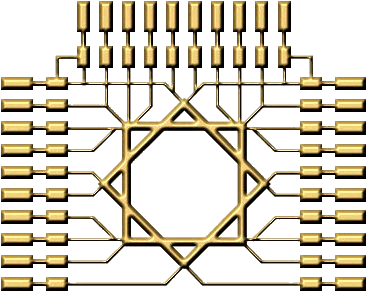
\includegraphics[width=0.2\linewidth]{images/HIAST_logo.png}}
		\label{}
	\end{figure}
	\begin{center}
		
		\large
		%\centering
		%\includegraphics[width=1\linewidth]{Figures/cover/HIAST.png}\\
		الجمهورية العربية السورية\\
		المعهد العالي للعلوم التطبيقية والتكنولوجيا\\
		قسم النظم الالكترونية
		\Large
		\vspace{3em}
		%\hline
		\vspace{3pt}
		%\hline
		\vspace{7pt}
		
		\textbf{
			الملاحقة بالاعتماد على تقنيات التعلم العميق\\
			\textLR{Visual Object Tracking Using Deep Learning Techniques}
		}
		\vspace{7pt}
		%\hline
		\vspace{3pt}
		%\hline
		
		
		\Large
		\vspace{1em}
		أعدت هذه الأطروحة لنيل\\
		درجة الماجستير في نظم  التحكم والروبوتيك\\
		
		
		\vspace{2em}
		\textbf{
			إعداد:\\
			م. مي عبود \\
			\vspace{2em}
			إشراف:\\
			د. آصف جعفر
			\hspace{4em}
			د. عمر حمدون\\
		}
		\vspace{4em}
		كانون الأول $ 2022 $
	\end{center}
	\begin{center}
		\textbf{إهداء}\\
		أهدي هذا العمل إلى أمي ...
		\newline
		وإلى روح أبي ...
		
	\end{center}
\end{titlepage}
\newpage

\newpage
\begin{center}
	\textbf{كلمة شكر}\\
أتوجه بالشكر الجزيل لكل من ساهم في إنجاح هذا العمل, وأخص بالذكر الدكتور آصف جعفر والدكتور عمر حمدون لما قدماه من وقت وجهد في الإشراف على البحث. 
\end{center}



\tableofcontents 
\listoffigures
\listoftables
\setlength{\parskip}{\baselineskip}
\begin{abstract}
يهدف هذا البحث إلى تطوير خوارزمية الملاحقة الحديثة 
\textLR{SwinTrack-Tiny}،
من خلال الاستفادة من المعلومات الزمانية. إذ أن مشكلة معظم الملاحقات الحديثة بما فيها الخوارزمية السابقة هي أنها تعتمد بشكل كامل على المعلومات المكانية كمعلومات مظهر الغرض في الصورة الابتدائية، وتتجاهل بشكل تام المعلومات الزمانية، كمعلومات تغير مظهر الغرض. بالإضافة إلى زمن التدريب الكبير للنماذج الحديثة التي تعتمد على تقنيات التعلم العميق.
\\
من أجل الاستفادة من المعلومات الزمانية، تم استخدام دخل ثالث لنموذج 
\textLR{SwinTrack-Tiny}
 وهو صورة الغرض الجديدة الناتجة عن الملاحقة. ولتجنب تدريب النموذج كاملا، قمنا بدمج سمات الـ
\textLR{template}
 الابتدائي مع صورة الغرض الجديدة باستخدام كتلة انتباه متعددة الرؤوس.
\\
وأظهرت الاختبارات التي تم إجراؤها على مجموعة المعطيات 
\textLR{GOT-10k}
 تحسناً في أداء النموذج بنسبة 
$0.8\% $
 للمعيار
\textLR{AO}
 و
$1.6\%$
  للمعيار 
$SR_{0.5}$،
 مع تغيير طفيف في سرعة الخوارزمية.
	
%تعد الملاحقة أحد أهم تطبيقات الرؤية الحاسوبية، وكغيرها من المجالات فقد تحسن أداء خوارزميات الملاحقة بفضل استخدام تقنيات التعلم العميق، لكن مشكلة معظم الملاحقات الحديثة هي أنها تركز على استخلاص السمات من الصورة بشكل فعال لتحديد مكان الغرض من خلال المعلومات المكانية أي معلومات المظهر فقط وتتجاهل المعلومات الزمانية مثل معلومات تغير مظهر الهدف، بالإضافة إلى بطء هذه الملاحقات بالمقارنة بالملاحقات التقليدية بسبب استخدام شبكات أو نماذج عميقة . وانطلاقاً من اهتمامنا بتطبيقات الزمن الحقيقي فقد اخترنا تطوير خوارزمية سريعة تحقق شروط الزمن الحقيقي في حال تشغيلها على العتاد الصلب المتوفر لدينا
%\textLR{GPU RTX 3060Ti}،
%ولذلك اخترنا خوارزمية 
%\textLR{SwinTrack-Tiny}
%والتي تعمل بسرعة أكثر من 
%$65 fps$.
%تم تطوير هذه الخوارزمية بإدخال المعلومات الزمانية إلى النموذج وذلك عن طريق إدخال 
%\textLR{template}
%الغرض المحدّث كدخل ثالث، وذلك كما في خوارزمية 
%\textLR{STARK}.
%هذا التعديل قد حسن أداء الخوارزمية بمقدار
%$0.8\%$ 
%من أجل معيار 
%$AO$,
%$1.6\%$
%من أجل معيار 
%$SR_{0.5}$
%مقارنة بالخوارزمية الأساسية،
%وذلك من أجل مجموعة المعطيات الخاصة بالملاحقة 
%\textLR{GOT-10k}،
%مع تغير طفيف في سرعة الخوارزمية.
%\newline
%الكلمات المفتاحية :
%ملاحقة غرض واحد، محول 
%\textLR{Swin},
%تابع الانتباه،
%تحديث الـ
%\textLR{template}.
\end{abstract}

\selectlanguage{english}
\begin{abstract}
	Tracking is one of the most important task in  computer vision. in recent years it has been improved by using deep learning techniques.
	most of the state-of-the-art trackers only focus on extracting effective features from object or search window image, ignoring temporal information. the other problem is slow speed due to use deep models comparing to traditional trackers. that is why in this research we choose a fast tracker to improve SwinTrack-Tiny tracker that achieve great performance and fast speed on GOT-10k dataset, almost twice faster than STARK tracker.
	this research aims to improve SwinTrack-Tiny by using temporal information entering updated template of object as a third input to the model, and fuse initiale template feature with dynamic template by using attention block to preserve weights of original model and train only attention block.
	our additiol block improve performance by $0.8\%$ for AO,$1.6\%$ $SR_{0.5}$ comparing to original tracker, with slightly affect speed.
	\newline
	Keywords : single object tracking, SOT, VOT, SwinTransformer, SwinTrack, STARK, attention, template, update template.
\end{abstract}
\selectlanguage{arabic}
%\chapter{مقدمة عامة}
\section{تمهيد}
ملاحقة الأغراض
\textLR{visual object tracking}
هي مجال من مجالات الرؤية الحاسوبية
\textLR{computer vision}،
والتي تهتم بتحديد حالة الغرض المراد ملاحقته في كل إطار من إطارات الفيديو. وهي موضوع بحث نشط لما تواجهه من الكثير من التحديات والمشكلات والتي تجعل من عملية الملاحقة مهمة صعبة، بالإضافة إلى تطبيقاتها في مجالات متنوعة مثل القيادة الذاتية، الطب، الرياضة، المجال العسكري، الأمن، الترفيه، وغيرها.


ظهر في العقود الأخيرة كم كبير من خوارزميات الملاحقة أبرزها
\textLR{NCC, Meanshift, MDNet, MOSSE}
وغيرها، والتي تستخدم تقنيات مختلفة لحل مشاكل الملاحقة. وبسبب تنوع الأساليب والتقنيات وكثرتها قررنا أن نركز في هذا البحث على خوارزميات الملاحقة التي تستخدم تقنيات التعلم العميق وذلك لعدة أسباب:
\begin{itemize}
	\item
تقنيات التعلم العميق هي الأكثر استخداماً في أبحاث الملاحقة في السنوات الأخيرة.
	\item
وجود العديد من معطيات التدريب الكافية لتدريب نماذج التعلم العميق مثل
\textLR{GOT-10k\cite{got10k}},
\textLR{LaSOT\cite{Lasot}}
		وغيرها.
	\item
تتصدر  ملاحقات التعلم العميق المراتب الأولى من حيث الأداء مقارنة بالملاحقات التقليدية.
	\item
ظهور العديد من ملاحقات التعلم العميق سريعة الأداء بشكل كافي لتطبيقات الزمن الحقيقي.
\end{itemize}
ظهرت في السنتين الأخيرتين بعض خوارزميات الملاحقة التي تستخدم المحول 
\textLR{Transformer\cite{Vaswani17}}
في بنيتها مثل
\textLR{STARK\cite{Stark}},
\textLR{SwinTrack\cite{swinTrack}},
وقد تفوقت في الأداء على خوارزميات الملاحقة الأخرى وقت ظهورها، بالإضافة إلى تحقيقها لمتطلبات الزمن الحقيقي في حال تشغيلها على وحدة معالجة رسومات 
$GPU$
كافية.
وبما أن المحول أعطى نتائج واعدة في مجال الرؤية الصنعية كما في خوارزمية الكشف 
\textLR{DETR\cite{DETR}}
فقد اخترنا في بحثنا التركيز على خوارزميات الملاحقة التي تستخدم المحول.
\newline
يسعى هذا البحث إلى التعرف على خوارزميات الملاحقة الحديثة بشكل عام، وإلى تقديم دراسة تفصيلية عن نموذج المحول، وتطوير نظام ملاحقة يعتمد في بنيته على المحول، مع الأخذ بعين الاعتبار سرعة الأداء.
\section{إشكالية ودوافع البحث}
ماتزال الملاحقة تواجه الكثير من التحديات والعقبات والتي تجعلها من المجالات الصعبة في الرؤية الحاسوبية.
إذ يتم تقييم خوارزميات الملاحقة من خلال قدرتها على تتبع الغرض الملاحَق وتجاوز التغيرات التي يعاني منها الغرض أو البيئة المحيطة به.


في هذه الفقرة سنذكر عدة مشكلات تواجه الملاحقة :
\textLR{\cite{Abbass21}}
\textLR{\cite{Zhang21}}
\textLR{\cite{got10k}}
\begin{itemize}
	\item
	تغيير الإضاءة.
	\item{الاحتجاب 
		\textLR{occlusion}
		: يمكن أن تحجب الخلفية جزء أو كامل الغرض.}
	\item
اختفاء الغرض كليا من المشهد.
	\item
تغير شكل الغرض بسبب طبيعته المفصلية.
	\item
تغير شكل الغرض بسبب تغير زاوية الرؤية.
	\item
حركة الكاميرا.
	\item{حركة الهدف إما بشكل سريع أو بشكل مفاجئ أو بسبب الدوران.}
	\item{وجود أغراض مشابهة للغرض المراد ملاحقته، أو وجود خلفية لها نفس بنية الغرض، وهذا ما يجعله يتماهى مع الخلفية, وبالتالي تزداد صعوبة الملاحقة.}
	\item{
		عدم وجود تفاصيل في الصورة إذ تكمن الصعوبة هنا في الحصول على عدد كاف من السمات لتوليد نموذج لمظهر الغرض 
		\textLR{appearance model}}.
	\item
	ملاحقة أغراض صغيرة.
	\item
	دقة الكاميرة المستخدمة.
	\item
		الملاحقة بالزمن الحقيقي، إذ تتطلب بعض التطبيقات أن تكون الملاحقة بأداء عالي وبسرعة كافية لمعالجة الصور بالزمن الحقيقي.
\end{itemize}
بالإضافة إلى التحديات المذكورة سابقاً فإن معظم الملاحقات الحديثة تستفيد فقط من معلومات مظهر الغرض والمنطقة المحيطة به أي المعلومات المكانية
\textLR{spatial information},
وتتجاهل المعلومات الزمانية
\textLR{temporal information}.
إذ أنها تعامل مسألة الملاحقة وكأنها مسألة كشف للأغراض دون الاستفادة من الإطارات المتلاحقة أو معلومات تغير المظهر.
\newline
الإشكالية الأخرى الناتجة عن اختيارنا لخوارزمية ملاحقة تعتمد على  التعلم العميق هي زمن التدريب الكبير للنموذج في حال عدم توفر عتاد صلب ذو إمكانيات قوية، بالإضافة إلى الحجم الكبير لمعطيات التدريب الخاصة بمسألة الملاحقة، فمثلاً حجم الملف الخاص بمجموعة المعطيات 
\textLR{GOT-10k\cite{got10k}}
يصل إلى أكثر من $60GB$.
\section{فكرة الحل المقترح}
من النقاط الأساسية التي يعالجها هذا البحث هي تطوير إحدى خوارزميات الملاحقة التي تعتمد فقط على المعلومات المكانية وتستخدم المحول وتحقق متطلبات الزمن الحقيقي وهي خوارزمية
\textLR{SwinTrack\cite{swinTrack}},
وذلك عن طريق الاستفادة من المعلومات الزمانية الناتجة عن تغير مظهر الغرض.
يتم ذلك عن طريق تطبيق دخل ثالث إلى الخوارزمية وهو صورة الغرض الجديدة
كما في خوارزمية 
\textLR{STARK\cite{Stark}},
ودمج سمات هذه الصورة مع سمات صورة الغرض الإبتدائية المأخوذة من أول إطار في عملية الملاحقة.
يتم هذا الدمج عن طريق تابع الانتباه
\textLR{Attention}،
وهو التابع الأساسي في نموذج المحول. هذا الدمج يضمن المحافظة على أبعاد نموذج الملاحقة الأساسي، وبالتالي يمكن الاستفادة من الأوزان المدربة سابقاً، تجنباَ لتدريب النموذج بالكامل، ونكتفي بتدريب كتلة الانتباه الإضافية فقط بسبب الإمكانيات المحدودة للعتاد الصلب المتوفر لدينا.
\section{المساهمات الأساسية في البحث}
الإضافات الجديدة التي يقدمها هذا البحث هي:
\begin{itemize}
\item
تطوير خوارزمية الملاحقة 
\textLR{SwinTrack\cite{swinTrack}}
عبر إدخال معلومات زمانية وهي صورة الغرض الجديدة كدخل ثالث.
\item
المحافظة على أبعاد النموذج الأساسي وذلك عن طريق استخدام كتلة انتباه لدمج سمات صورة الغرض الإبتدائية مع صورة الغرض الجديدة.
\item
تدريب كتلة الانتباه باستخدام مجموعة المعطيات الخاصة بمسألة الملاحقة
\textLR{GOT-10k\cite{got10k}}.
\item
اختبار إضافة كتلة انتباه بثمانية رؤوس وبأربعة رؤوس.
\item
تحسين الأداء مع المحافظة على متطلبات الزمن الحقيقي.
%\item
%وعلى المستوى العملي تعديل الكود الأساسي للخوارزمية بإضافة تابع لتجريب خوارزمية الملاحقة
%\textLR{SwinTrack\cite{swinTrack}}
%من أجل فيديوهات.
\end{itemize}
\section{مخطط البحث}
يتضمن هذا البحث عدة فصول، يبدأ الفصل الثاني بتعريف مسألة الملاحقة، ويحتوي على دراسة مرجعية لتصنيف خوارزميات الملاحقة التي تستخدم تقنيات التعلم العميق. ثم نقدم دراسة نظرية تفصيلية لنموذج المحول ولتابع الانتباه، وذكر تطبيقاته في مجال الرؤية الصنعية مثل الكشف والتصنيف ونخص بالذكر تطبيقاته في مجال الملاحقة، وأخيراً نقوم بشرح محول 
\textLR{Swin\cite{swintransformer}}،
وهو النموذج المعتمد لاستخلاص سمات الصور باعتباره
\textLR{backbone}.
\newline
أما في الفصل الثالث سنقوم بعرض النماذح الأساسية التي اعتُمِد عليها وهي خوارزمية 
\textLR{STARK\cite{Stark}}
وخوارزمية
\textLR{SwinTrack\cite{swinTrack}}،
ثم نعرض التعديل المقترح.
\newline
في الفصل الرابع نعرض نتائج التجارب التي قمنا بها، مع شرح عن مجموعة المعطيات الخاصة بالتدريب والاختبار،
وفي الفصل الخامس والأخير نذكر الخاتمة والآفاق المستقبلية بالإضافة إلى الصعوبات التي واجهتنا في هذا المشروع.



%\chapter{دراسة نظرية ومرجعية}
\section{مقدمة}
يعرض هذا الفصل مقدمة عن مفهوم الملاحقة وعن أنواعها، بالإضافة إلى دراسة مرجعية بأنواع خوارزميات الملاحقة فيما يخص التعلم العميق، ثم ننتقل إلى شرح نموذج المحول كونه الكتلة الأساسية في خوارزمية الملاحقة 
\textLR{SwinTrack\cite{swinTrack}},
بحيث نبدأ بشرح عام عن النماذج السابقة له، وكيفية تطور بنيته، ونعرض بالتفصيل تابع الانتباه وهو التابع المستخدم في عملية دمج السمات في نموذجنا المقترح.
ومن ثم نستعرض تطبيقات المحول في الرؤية الصنعية مثل الكشف والتصنيف ونركز على تطبيقاته في الملاحقة, وأخيراً نتحدث بالتفصيل عن محول 
\textLR{Swin}
كونه النموذج المعتمد في استخلاص السمات.
\section{تعريف مفهوم الملاحقة
\textLR{\cite{Abbass21}}
\textLR{\cite{Zhang21}}
}
نهتم في بحثنا بملاحقة غرض واحد
\textLR{single object tracking}
  دون معلومات مسبقة عن هذا الغرض 
\textLR{general object tracking}.
  في هذه الحالة نعرف عملية الملاحقة بأنها تقدير لحالة الغرض المراد ملاحقته في الصور المتلاحقة للفيديو بالاعتماد فقط على مظهره في الإطار الأول. يمكن التعبير عن حالة الغرض بمستطيل محيط به في كل إطار من إطارات الفيديو، ندعوه بالـ مستطيل المحيط
\textLR{bounding box}،
يتم تحديده يدويا في الإطار الأول. ونسمي ما بداخل المستطيل المحدد يدويا في الإطار الأول بالـ
\textLR{template}
 قالب.
بعد تحديد الـ
\textLR{template}
 في الإطار الأول للملاحقة يأتي إطار جديد من الفيديو والمهمة هي تقدير المستطيل المحيط. من أجل الإطار الجديد نقوم باقتطاع المنطقة المحيطة بموقع الهدف في الإطار السابق بحجم معين ( مثلا أربع أضعاف المستطيل المحيط السابق) ونسمي هذه المنطقة بنافذة البحث 
\textLR{search window}،
لأننا لا نبحث عن الهدف في كامل الصورة ولكن فقط في هذه المنطقة.
%معظم الملاحقات تتبع إطار العمل المشروح سابقاً والموضح في الشكل التالي:
%
%صورة توضيحية ****

\section{أنواع خوارزميات الملاحقة}
يمكن تصنيف خورازميات الملاحقات بشكل عام كما يلي :

\begin{itemize}
	\item
هل هي قصيرة المدى أم بعيدة المدى
\begin{itemize}
\item
خوارزميات ملاحقة قصيرة المدى
\textLR{short-term trackers}:
مهمتها هي تقدير حالة الغرض
حتى تفشل عملية الملاحقة، وتكون عملية إعادة الملاحقة غير مطلوبة. عادة يتم تقييمها على فيديوهات قصيرة لا تتجاوز 
\textLR{1000}
إطار.
\item
خوارزميات ملاحقة البعيدة المدى 
\textLR{long-term trackers}:
من ضمن أهدافها إعادة الملاحقة في حال الفشل أو في حال اختفاء الغرض من مجال الرؤية. عادة يتم تقييمها على فيديوهات طولها  
\textLR{10000-1000}
		  إطار.
\end{itemize}
\item مسألة ملاحقة بكاميرا واحدة أو عدة كاميرات
\item 
ملاحقة هدف واحد 
\textLR{SOT}
% \selectlanguage{english}
%\begin{figure}[H]
%	\centering
%	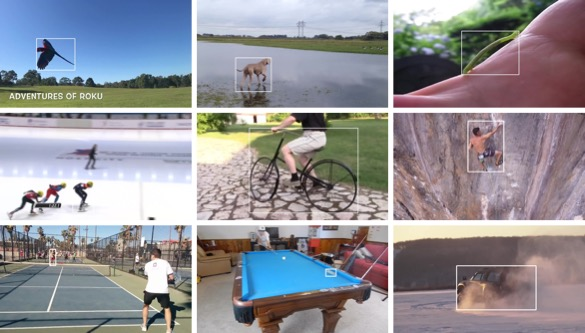
\includegraphics[width=\textwidth]{images/got10k}
%	\caption{
%		VOT
%		\textRL{لأغراض}
%		got10k \cite{got10k}
%		\textRL{عينات من مجموعة معطيات التدريب}
%	}	
%\end{figure}
%\selectlanguage{arabic}
أو
 عدة أهداف
\textLR{MOT}
%\selectlanguage{english}
%\begin{figure}[!h]
% 	\centering
% 	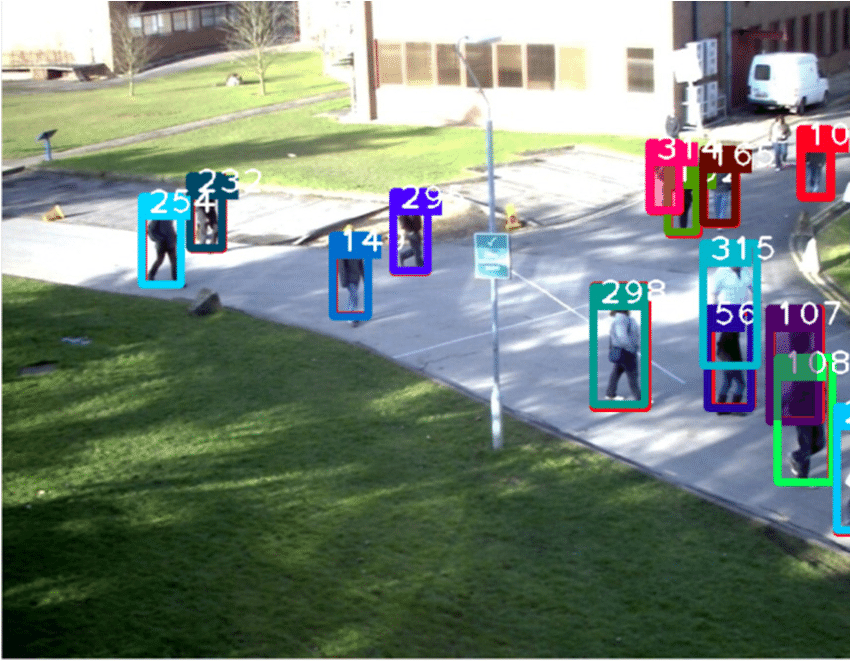
\includegraphics[width=\textwidth]{images/MOT15}
% 	\caption{
%		MOT
%		\textRL{لأغراض}
% 		\cite{Mot15}
% 		Mot15
% 		\textRL{ مثال عن مجموعة معطيات التدريب}
% 	}	
%\end{figure}
%\selectlanguage{arabic}
\item
ملاحقة سببية أو فورية
 \textLR{online tracker}،
غير سببية أو مؤجلة
 \textLR{offline tracker}:
\begin{itemize}
\item
خوارزميات ملاحقة غير سببية:
في بعض التطبيقات  كتحليل الفيديو مثلا، لا نحتاج إلى معرفة مكان الغرض  بشكل لحظي، عندها يمكن معالجة كامل صور  الفيديو دفعة واحدة، إذ يكون التركيز على دقة الملاحقة أكثر  من سرعة عملية المعالجة. وسميت بالملاحقات غير السببية لأن نتيجة الملاحقة لإطار معين يمكن أن تعتمد على الإطارات اللاحقة.
	
\item
خوارزميات ملاحقة سببية:
خرج الملاحقة من أجل الإطار الحالي يعتمد فقط على الإطارات السابقة، وهو الأكثر انتشاراً كون معظم تطبيقات الملاحقة تتطلب الحصول على النتيجة بشكل فوري.
	
\end{itemize}
\end{itemize}
نهتم في بحثنا بخوارزميات الملاحقة السببية، كاميرا واحدة، قصيرة المدى، و بالملاحقة بالزمن الحقيقي.
\section{أنواع خوارزميات الملاحقة التي تعتمد  التعلم العميق}
يمكن تصنيف ملاحقات التعلم العميق بحسب المرجع
\textLR{\cite{Marvasti}}
 كما يلي:
 \subsection{بنية الشبكة المستخدمة}
 إما أن تكون شبكات
 \textLR{Transformer,GAN,RNN,SNN,CNN}
 أو شبكة مصممة خصيصا لغرض الملاحقة
 \subsubsection{
 	الشبكات العصبونية التلافيفية
 \textLR{CNN Convolutional Neural Networks}}
استخدمت الشبكات التلافيفية في كثير من خوارزميات الملاحقة وذلك لقدرتها على إعطاء تمثيل للغرض بشكل أفضل من الشبكات الأخرى في حال وجود معطيات تدريب كافية،
لكنها غير ملائمة للتدريب أثناء الملاحقة
\textLR{online training}
بسبب التعقيد الحسابي الكبير.
مثل ملاحق 
 \textLR{MDNet \cite{MDNet}}.
 \begin{figure}[h!]
 	\centerline{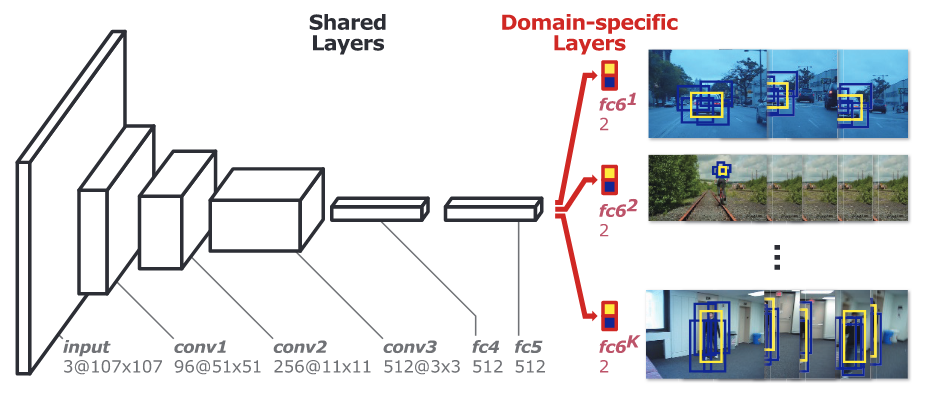
\includegraphics[width=\textwidth]{images/MDNet}}
 	\caption{\textRL{بنية الملاحق}
		\textLR{MDNet} 		 		
 		\textRL{الذي يستخدم شبكات تلافيفية}
 		\textLR{\cite{MDNet}}}	
 \end{figure}
\subsubsection{الشبكات التوأمية 
\textLR{SNN Siamese Neural Networks}}
سميت الشبكات التوأمية بذلك لأنها تتكون من شبكتين متطابقتين في البنية و الأوزان. في معظم تطبيقات الملاحقة يكون دخل الشبكة الأولى هو 
\textLR{template}
الغرض، أما دخل الشبكة الثانية فهو نافذة البحث. انتشر استخدام هذا النوع من الشبكات في خوارزمية الملاحقة بالزمن الحقيقي، لأنها ليست بحاجة إلى تعديل الأوزان أثناء الملاحقة، إذ يكفي تدريب الشبكة بشكل 
\textLR{offline}.
من الممكن أيضاً استخدام أي نوع من الشبكات ضمن الشبكة التوأمية مثل الشبكات التلافيفية كخوارزمية 
\textLR{GOTURN\cite{GOTURN}}
الموضحة في الشكل 
\ref{fig:GOTURN},
أو كمحول 
\textLR{Swin\cite{swintransformer}}
كما في 
\textLR{SwinTrack\cite{swinTrack}}
وهو النموذج الأساسي في بحثنا.
\begin{figure}[h!]
	\centerline{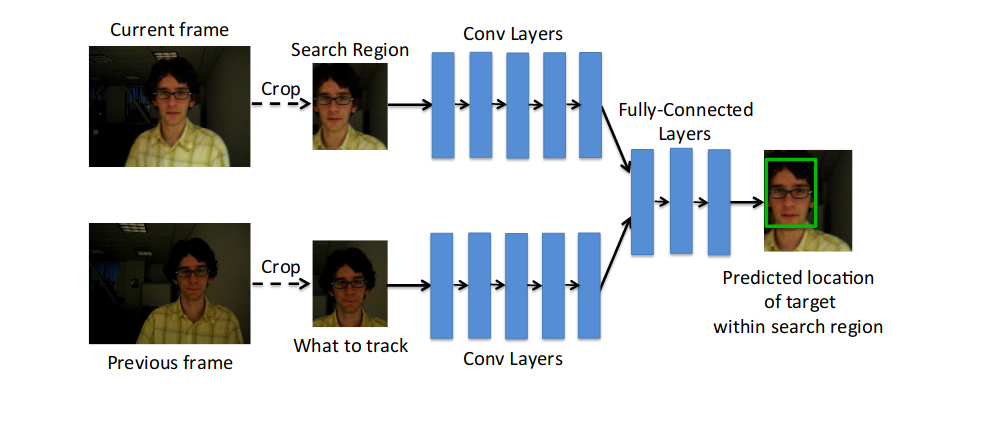
\includegraphics[width=\textwidth]{images/GOTURN}}
	\caption{
		\textRL{بنية الملاحق}
		\textLR{GOTURN}
		\textRL{الذي يستخدم شبكة توأمية مع تلافيفية}
		\textLR{\cite{GOTURN}}}	
	\label{fig:GOTURN}
\end{figure}
\subsubsection{الشبكات العصبونية العودية
\textLR{RNN Recurrent Neural Networks}}
بما أن الملاحقة لاتتعلق فقط بالمعلومات المكانية بل أيضاً بالمعلومات الزمانية، تم استخدام شبكات 
\textLR{RNN}
في مجال الملاحقة ولكن  بشكل محدود، نذكر منها خوارزمية 
\textLR{FPRNet}
\textLR{\cite{Ma18}}

\subsubsection{المحول 
\textLR{Transformer}}
لاقى نموذج المحول نجاحاً كبيراً في مجال معالجة اللغات الطبيعية 
\textLR{\cite{Vaswani17}}،
وبسبب هذا النجاح تم استخدامه في تطبيقات الرؤية الصنعية مثل كشف الأغراض كما في خوارزمية
\textLR{DETR\cite{DETR}}.
 وقد تم استغلاله لأغراض الملاحقة في العامين الأخيرين كما في خوارزميات 
\textLR{STARK\cite{Stark},
TrTr\cite{TrTr} ,
SwinTrack \cite{swinTrack}}.
\subsection{التدريب}
إما أن يكون التدريب 
\textLR{Online}
أو
\textLR{Offline}
 أو كلاهما معاً.
 الكثير من خوارزميات التعلم العميق تستفيد من خرج الشبكات المدربة مسبقاً على مهام مشابهة، والملاحقة مسألة مشابهة لكشف أو تصنيف الصور، لذلك نرى العديد من خوارزميات الملاحقات تستخدم شبكات مثل 
\textLR{ResNet\cite{ResNet},
VGG\cite{VGG}}
كـ
\textLR{backbone}
لاستخلاص السمات من الصور.


يمكن الاستفادة من بعض طبقات هذه الشبكات، أو تعديل بعض أو كل الأوزان بإجراء ضبط نهائي
\textLR{fine tuning}.
\subsubsection{
التدريب بشكل
\textLR{offline}}
معظم ملاحقات التعلم العميق تقوم بعملية التدريب بشكل
\textLR{offline}
وذلك بالاستفادة من مجموعات المعطيات الخاصة بالملاحقة مثل مجموعة المعطيات
\textLR{GOT-10k\cite{got10k},
	 LaSOT\cite{Lasot},
	 TrackingNet\cite{Trackingnet}}
وغيرها.
إذ أن التدريب بشكل  
\textLR{offline}
مناسب لتطبيقات الزمن الحقيقي لأن أوزان النموذج لاتحتاج إلى تعديل أثناء عملية الملاحقة، كما أن ذلك يقلل من انحياز النموذج نحو أغراض معينة 
\textLR{overfitting}
نتيجة التدريب بشكل 
\textLR{online}.
معظم الملاحقات الحديثة يتم تدريبها فقط بشكل 
\textLR{offline}
مثل
\textLR{
STARK\cite{Stark},
SiamRPN++\cite{SiamRPN++},
SwinTrack\cite{swinTrack}}
وغيرها الكثير.
\subsubsection{
التدريب بشكل 
\textLR{Online}
}
من المعروف أن تدريب نماذج التعلم العميق يحتاج زمن طويل وقدرة حسابية عالية، وفي حال عدم توفر عتاد صلب ملائم للتدريب من الممكن اللجوء إلى التدريب بشكل
\textLR{online}
لبعض النماذج، وذلك بتعديل بعض أو كامل أوزان النموذج.
نذكر منها خوارزمية 
\textLR{DeepTrack\cite{DeepTrack},SMART\cite{SMART}}.

\subsubsection{التدريب 
\textLR{online}
و 
\textLR{offline}
معاً}
يمكن جمع طريقتي التدريب السابقتين وذلك بتدريب النموذج بشكل
\textLR{offline}
في البداية
باستخدام مجموعات المعطيات الخاصة بالملاحقة، وبعد ذلك يتم تعديل كامل أو بعض أوزان النموذج أثناء عملية الملاحقة. وذلك كما في خوارزميات 
\textLR{ATOM\cite{ATOM},
	 MDNET\cite{MDNet},
	 DiMP\cite{DIMP},
	 PrDiMP\cite{prDIMP}}.
\subsubsection{}
و كغيرها من نماذج تعلم الآلة فإن خوارزميات الملاحقة التي تعتمد تقنيات التعلم العميق تستخدم تعزيز المعطيات
\textLR{data  augmentation}
 لتقليل الـ
\textLR{ overfitting}،
 وهي طريقة لزيادة حجم مجموعة المعطيات باستخدام بعض التقنيات كاستخدام تحويلات إما في الفضاء الهندسي أو اللوني أو غيرها.
\subsection{غرض الشبكة}
إما أن يكون غرض الشبكة التصنيف 
\textLR{classification}
 أو الـ 
\textLR{regression}
 أو كلاهما معاً.

\subsubsection{التصنيف}
تستخدم الكثير من  الملاحقات أساليب الخوارزميات الأخرى المشابهة لها في  المهام ككشف أو تصنيف الأغراض في الصور وغيرها، ومن هذه الأساليب هي توليد العديد من المناطق المرشَّحة تدعى بـ
\textLR{candidates}
أو بـ
\textLR{proposal bounding boxes}
 المستخلصة من نافذة البحث، ويكون هدف الشبكة هو تصنيف هذه المناطق إما كغرض أو كخلفية. وبالتالي يدرب النموذج وفق هذا المعيار وتستخدم العديد من توابع الخسارة لهذا الغرض مثل 
\textLR{cross-entropy CE,
	focal loss FL\cite{FocalLoss}،
	varifocal loss VL\cite{varifocal}}،
وغيرها، كملاحقات 
\textLR{SiamFC\cite{SiamFC} , DeepTrack\cite{DeepTrack}}.
\subsubsection{
\textLR{Regression}
}
غرض الشبكة في هذه الحالة هو تحديد مكان وأبعاد المستطيل المحيط للغرض بشكل مباشر باستخدام توابع خطأ تعتمد على
\textLR{L1}
 أو
\textLR{L2}،
كما في 
\textLR{GOTURN\cite{GOTURN}}.

\subsubsection{التصنيف والـ
\textLR{regression}
معاً}
 العديد من الملاحقات  قد استخدمت كلتا الطريقتين للتنبؤ بمكان الهدف، إذ يتم توليد العديد من المناطق المرشحة وتحديد المنطقة الأكثر شبهاً بالغرض من خلال شبكة تصنيف، وتحديد أبعاد المستطيل المحيط و زيادة دقة التنبؤ بموقع الغرض من خلال شبكة 
\textLR{regression}،
كما في 
\textLR{MDNet\cite{MDNet}, SwinTrack\cite{swinTrack}, DiMP\cite{DIMP}, SiamRPN++\cite{SiamRPN++}} 
وغيرها.
\subsection{خرج الشبكة}
تبعاً لغرض الشبكة فإن الخرج يمكن أن يكون
\begin{itemize}
	\item خريطة الاستجابة: او ما يدعى بـ 
	\textLR{Confidence}
أو
	\textLR{Response Map}
وهي عبارة عن مصفوفة من القيم ضمن المجال
	$[0,1]$،
وكل قيمة تعبر عن احتمالية وجود الغرض  في الموقع المقابل لها	كما في 
	\textLR{SiamFC\cite{SiamFC}, ATOM\cite{ATOM}, DiMP\cite{DIMP}, SMART\cite{SMART}, PrDiMP\cite{prDIMP}}.
	\item 
	المستطيل المحيط بالغرض: ويمكن أن يعبر عنه بإحداثيات زاويتي المستطيل المتقابلتين، أو بإحداثيات المركز مع أبعاد المستطيل،
	كما في 
	\textLR{GOTURN\cite{GOTURN}, SiamRPN++\cite{SiamRPN++}}
	\item 
	نتيجة التشابه
		 \textLR{similarity score}
		 مثل
		 \textLR{MDNet\cite{MDNet}, DeepTrack \cite{DeepTrack}, SiamRPN++ \cite{SiamRPN++}}
	\item 
	قناع التجزئة
	\textLR{Segmentation Mask}
	مثل خوارزمية 
	\textLR{SiamAttn \cite{SiamAtt}}.
\end{itemize}
هذا فيما يخص أنواع خوارزميات الملاحقة، في الفقرة التالية سنشرح عن نموذج المحول، وعن النماذج السابقة له وكيفية تطور بنيته، وسنشرح عن تابع الانتباه 
\section{النماذج السابقة للمحول}
صمم نموذج المحول
\textLR{\cite{Vaswani17}}
ليكون إحدى نماذج
\textLR{seq2seq}،
وهي نماذج يكون كل من دخلها وخرجها عبارة عن سلاسل من العناصر. من الممكن أن تكون السلسلة أي نوع من المعلومات ككلمات، صور، محارف أو غيرها
\textLR{\cite{web:visualize}}.
\newline
معظم تطبيقات نماذج
\textLR{seq2seq}
 كانت في مجال معالجة اللغات الطبيعية
\textLR{Natural Language Processing NLP}
 أي يكون الدخل عبارة عن سلسلة من كلمات.
\begin{figure}[h!]
\centerline{
	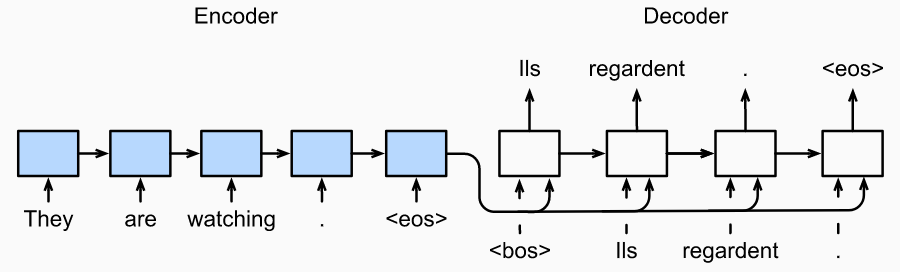
\includegraphics[width=\textwidth]{images/RNN.png}}
\caption{نموذج
\textLR{seq2seq}
مع بنية
\textLR{encoder-decoder}
\textLR{\cite{d2l_rnn}}
}
\label{fig:RNN1}	
\end{figure}
%قبل استخدام نموذج المحول
كانت البنية الأساسية لنماذج
\textLR{seq2seq}
هي الشبكات العصبونية العودية
\textLR{recurrent neural networks RNN}.
ولفهم تطور بنية المحول يجب أن نفهم البنية العامة للشبكات العودية وهو ما سنذكره في الفقرة القادمة.
\newline
\subsection{الشبكات العصبونية العودية
\textLR{RNN}
}
تُستخدم
\textLR{RNN}
 بشكل رئيسي للتعرف على الأنماط في المعطيات التسلسلية، كالنصوص، الفيديوهات أو أي متسلسلة زمنية. وما يميزها
 عن الشبكات العصبونية التقليدية
\textLR{MLP Multilayer perceptron}
 هو كيفية مرور المعلومات من خلالها
\textLR{\cite{RNN-gentleIntro}}.

\begin{figure}[H]
	\centerline{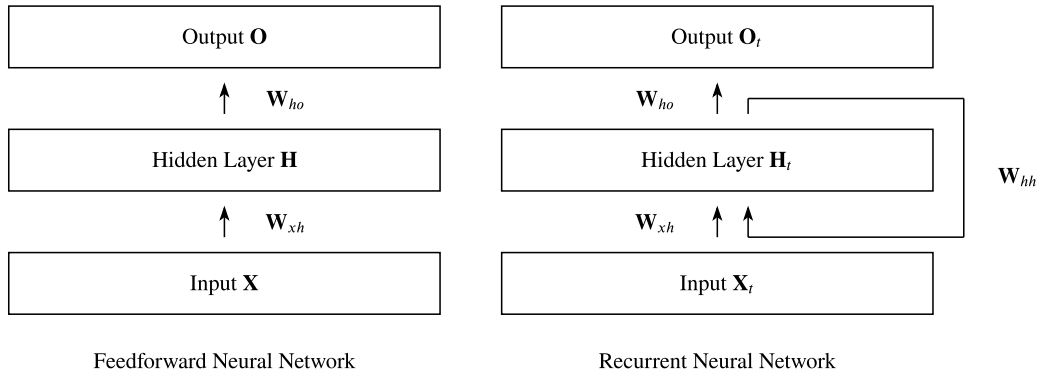
\includegraphics[width=\textwidth]{images/RNN_gentle_introduction.png}}
	\caption{
	\begin{footnotesize}
			الفرق بين مرور المعلومات بين الشبكات العودية - اليمين، والشبكات التقليدية - اليسار
\textLR{\cite{RNN-gentleIntro}}
	\end{footnotesize}
		}
	\label{fig:RNN2}
\end{figure}
يوضح الشكل
\ref{fig:RNN2}
 الاختلاف بين
\textLR{MLP}
 و
\textLR{RNN}،
 حيث تمرر شبكات 
\textLR{MLP}
المعلومات بدون وجود أي حلقات على العكس من شبكات
\textLR{RNN}.
حيث يحسب الخرج في شبكات
\textLR{MLP}
 كما في المعادلات
\ref{eq:mlp}
\begin{equation}
	\begin{split}
	& H = \phi_h (XW_{xh} + b_h)\\
	& O = \phi_o (HW_{ho} + b_o)\\
	\end{split}
	\label{eq:mlp}
\end{equation}
حيث $H$ خرج الطبقة المخفية، 
$\phi_h$
تابع تفعيل الطبقة المخفية،
$O$
الخرج النهائي،
$\phi_o$
تابع تغعيل طبقة الخرج، 
$W,b$
مصفوفات الأوزان وأشعة الانحياز.
\newline
أما في 
\textLR{RNN}
فمعادلة الخرج في كل خطوة زمنية
$t$
تحسب من خلال المعادلات 
\ref{eq:RNN}
\begin{equation}
\begin{split}
	&H_t = \phi_h(X_t W_{xh} + H_{t-1} W_{hh} + b_h)\\
	& O_t = \phi_o (H_t W_{ho} + b_o)\\
\end{split}
\label{eq:RNN}
\end{equation}
حيث
$H_t$
يدعى بالحالة المخفية
\textLR{hidden state}
في اللحظة
$t$.
\newline
نلاحظ أنه في كل خطوة زمنية لحساب الخرج نحتاج إلى الدخل
$X_t$
وإلى الحالة المخفية في الخطوة الزمنية السابقة كما هو موضح في الشكل 
\ref{fig:RNN3}،
والذي يبين مخارج ومداخل
\textLR{RNN}
بعد نشر الشبكة من أجل كل خطوة زمنية.
\begin{figure}[h!]
	\centerline{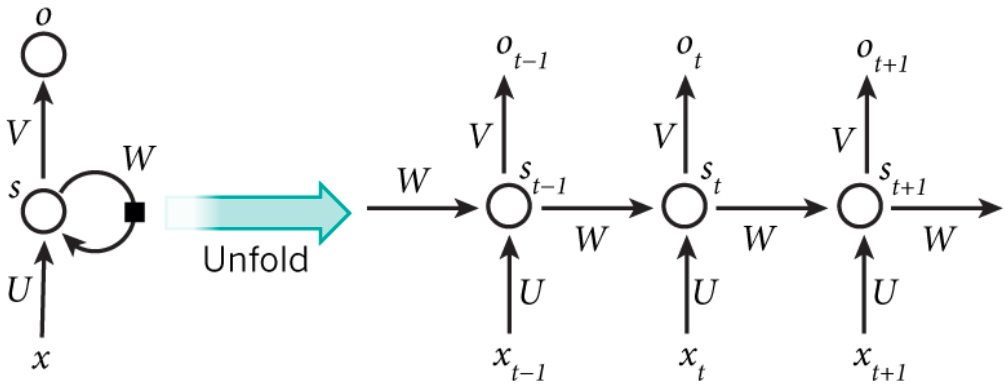
\includegraphics[width=\textwidth]{images/RNN_unfold}}
	\caption{
		نشر الشبكة العصبونية العودية
		\textLR{RNN}
		من أجل عدة لحظات زمنية
		\textLR{\cite{RNN-unfold}}}
	\label{fig:RNN3}
\end{figure}
%نلاحظ أيضا أنه لحساب الخرج في لحظة زمنية
%$t$
%نحتاج إلى دخل السلسلة في هذه اللحظة
%$X_t$
%وإلى الحالة المخفية في اللحظة السابقة
%$H_{t-1}$
%أو
%$s_{t-1}$
%كما هو موضح في الشكل
%\ref{fig:RNN3}
%والمعادلات
%\ref{eq:RNN}.
\newline
\subsubsection{مشكلات 
\textLR{RNN}}
إحدى سلبيات شبكات
\textLR{RNN}
 هي معالجة العناصر بشكل تسلسلي، فكما رأينا في الفقرة السابقة فإن الخرج في كل خطوة زمنية يحتاج إلى معالجة المداخل السابقة بشكل تسلسلي و هذا مايجعل زمن التدريب طويلاً، وبسبب بنية الشبكة تصبح المعالجة بشكل تفرعي أمراً صعباً أو حتى مستحيل
\textLR{\cite{TransformerCV}}.
المشكلة الثانية هي تلاشي المشتقات
\textLR{vanishing gradient}
وهو ما يزيد من صعوبة التدريب وبخاصة في حالة السلاسل الطويلة، إحدى أشهر الحلول لتقليل أثر هذه المشكلة هي باستخدام
\textLR{Long Short-Term Memory LSTM}.
من الممكن أن تختلف أبعاد سلسلتي الدخل والخرج ولحل هذا الاختلاف في الطول يمكن استخدام شبكتين عوديتين منفصلتين الأولى نسميها الـ
\textLR{encoder}
المرمز والثانية الـ
\textLR{decoder}
مفكك ترميز.
\subsection{
بنية المرمز ومفكك الترميز
}
يعالج المرمز كل عنصر من عناصر سلسلة الدخل ويستخرج المعلومات ويضعها في شعاع يسمى شعاع السياق
\textLR{context vector}،
بعد انتهاء المرمز من معالجة كامل عناصر الدخل يرسل شعاع السياق إلى مفكك الترميز
%\textLR{decoder}
 ليقوم بتوليد سلسلة الخرج بشكل تتابعي كما في الشكل
\ref{fig:RNN1}.
\newline
المشكلة الأساسية في هذه النماذج هي كيفية توليد شعاع السياق ليعبر بأفضل طريقة ممكنة عن معلومات سلسلة الدخل. فإذا كان شعاع السياق هو الحالة المخفية لآخر خطوة زمنية في سلسلة الدخل عندها لن يعبر بشكل فعال عن بدايات السلسلة وخصوصاً في حالة سلسلة الدخل الطويلة
\textLR{\cite{IllustratedAttention}}.
عندها يمكن أن يكون شعاع السياق عبارة عن كامل الحالات المخفية لكل خطوة زمنية في سلسلة الدخل، أو أن ينتج عن تعديل هذه الحالات المخفية بتطبيق تابع معين، ومن هنا ظهرت فكرة الانتباه 
\textLR{attention}،
وذلك بالتركيز فقط على الأجزاء المهمة وجعل الأجزاء غير المهمة أقل تأثيراً
\textLR{\cite{TransformerCV}}.
بما أن المشكلة الأساسية هي كيفية توليد شعاع السياق كان هناك الكثير من الأبحاث لتحسين تمثيل هذا الشعاع من أبرزها
\textLR{\cite{Bahdanau2016},\cite{Luong2015}}.
إذ كانت هذه الأعمال بدايات فكرة الانتباه، والذي أظهر نتائج جيدة ومبشرة في تطبيقات ترجمة الآلة، وخاصة في حالة الأبعاد الكبيرة لسلاسل الدخل
\textLR{\cite{IllustratedAttention}}.

\section{المحول \label{section:transformer}}
ظهر نموذج المحول
\textLR{Transformer\cite{Vaswani17}}
في عام $2017$ ولأول مرة تم اختبار نموذج يعتمد بشكل كامل على توابع الانتباه ويستغني عن
\textLR{RNN}،
 مما جنب نموذج المحول العديد من مشاكل هذا النوع من الشبكات والتي أهمها عدم القدرة على المعالجة التفرعية لعناصر الدخل، إذ أن أحد ميزات المحول هي قابلية معالجة العمليات الحسابية بشكل تفرعي كما سنرى لاحقاً وهذا ما يسرع عملية التدريب و الـ 
\textLR{inference}
في حال وجود
\textLR{GPU}.
\subsection{بنية المحول}
\begin{table}[h!]
	\centering
	\begin{tabular}{c c} 
		\hline
		\textLR{sympol} & \textLR{meaning} \\ [0.5ex] 
		\hline\hline
		$d$ & \textRL{بعد النموذج}  \\ 
		$h$ &  \textLR{MHA} \textRL{عدد الرؤوس في}\\
		$L$ & \textLR{tokens} \textRL{عدد عناصر سلسلة الدخل، أو عدد الـ}\\
		$X \in \mathds{R}^{L \mathsf{x}d}$&\textRL{دخل المرمز}\\
		$W^k \in \mathds{R}^{d \mathsf{x} d_x}$&\textLR{key}\textRL{مصفوفة الأوزان لشعاع الـ }\\
		$W^q \in \mathds{R}^{d \mathsf{x} d_x}$&\textLR{query}\textRL{مصفوفة الأوزان لشعاع الـ }\\
		$W^v \in \mathds{R}^{d \mathsf{x} d_v}$&\textLR{value}\textRL{مصفوفة الأوزان لشعاع الـ }\\
		$W^k_i,W^q_i \in \mathds{R}^{d\mathsf{x}d_k/h};W^v_i\in \mathds{R}^{d\mathsf{x}d_v/h}$&\textRL{مصفوفات الأوزان لكل  رأس}\\
		$W^o \in \mathds{R}^{d_v \mathsf{x}d}$&\textRL{مصفوفة الأوزان لشعاع الخرج }\\
		$Q = XW^q \mathds{R}^{L \mathsf{x}d_k}$&\textLR{query}\\
		$K = XW^k \mathds{R}^{L \mathsf{x}d_k}$&\textLR{key}\\
		$V = XW^v \mathds{R}^{L \mathsf{x}d_v}$&\textLR{value}\\
		\hline
	\end{tabular}
	\caption{\textRL{الرموز المستخدمة في شرح بنية المحول مع أبعاد المصفوفات}}
	\label{table:transformer_sympols}
\end{table}          
إن التطبيق الأساسي لنموذج المحول الأصلي
\textLR{\cite{Vaswani17}}
هو ترجمة الجمل من اللغة الإنكليزية إلى لغات أخرى، إذ أن دخل النموذج سلسلة من الكلمات (عدة جمل)، كل كلمة يتم التعبير عنها بشعاع من الأرقام ندعوه بالـ
\textLR{token}،
فيكون دخل المرمز هو عبارة عن مصفوفة أشعة
$X \in \mathds{R}^{L \mathsf{x}d}$.
\newline
لتمييز مكان كل عنصر من السلسلة  يتم إضافة قيم للترميز المكاني
\textLR{positional encoding PE}.
خرج كل طبقة من طبقات المرمز وطبقات مفكك الترميز
هو مصفوفة أشعة بأبعاد
$L \mathsf{x} d$.
كما يوضح الشكل
\ref{fig:Transformer}
يتكون كل من المرمز و مفكك الترميز
 من عدة كتل متسلسلة ومتطابقة في البنية.
\subsection{المرمز}
بداخل كل كتلة مرمز كتلتان أساسيتان كما في الشكل
\ref{fig:enc_dec}
 الأولى لحساب الانتباه الذاتي متعدد الرؤوس 
\textLR{Multi-Head Self Attention MHA},
مهمة هذا التابع هو تعديل تمثيل عناصر سلسلة الدخل بحسب السياق.
والكتلة الثانية هي شبكة عصبونية
\textLR{FFN}
تتكون من طبقتين مع تابع تفعيل 
\textLR{ReLU}
بحسب المعادلة
\ref{eq:MLP}.
\begin{equation}
FFN(x) = max(0,xW_1+b_1)W_2+b_2
\label{eq:MLP}
\end{equation}
تطبق هذه الشبكة على كل
\textLR{token}
أو عنصر دخل بشكل منفصل ومتطابق، وهذا مانسميه
\textLR{position-wise}
كما في الشكل
\ref{fig:positionWise}،
مما يجعل المحول قادر على إجراء الحسابات بشكل تفرعي.
من أجل كل من الكتلتين السابقتين يتم تطبيق
\textLR{residual connection \cite{residual}}،
 متبوعة بـ
\textLR{layer normalization\cite{LN}}.
\newline
%$\text{\textLR{LayerNorm}}(x+\text{\textLR{Sublayer}}(x))$
%حيث
%\textLR{sublayer}
%هي تابع الانتباه أو الشبكة العصبونية الأمامية.
\begin{figure}[H]
	\centerline{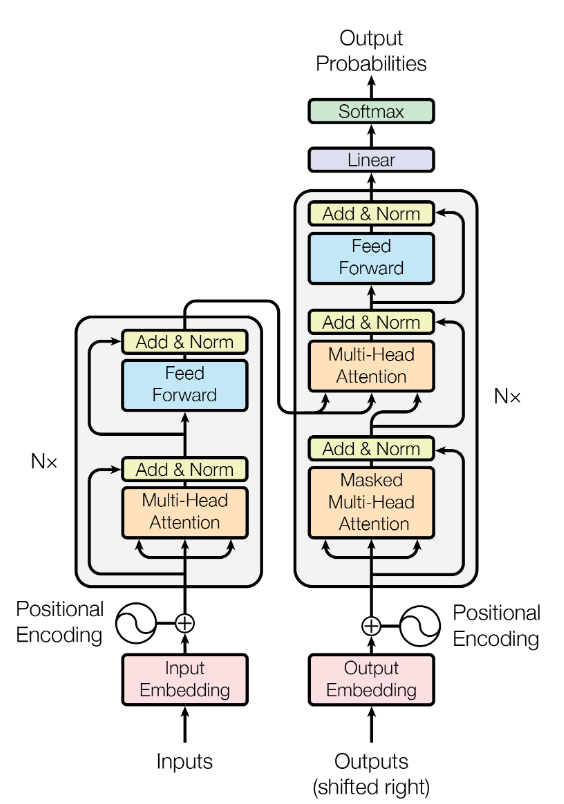
\includegraphics[scale=0.5]{images/Transformer}}
	\caption{\textRL{البنية الأساسية للمحول}
	\textLR{\cite{Vaswani17}}}
	\label{fig:Transformer}
\end{figure}

\begin{figure}[h!]
	\centerline{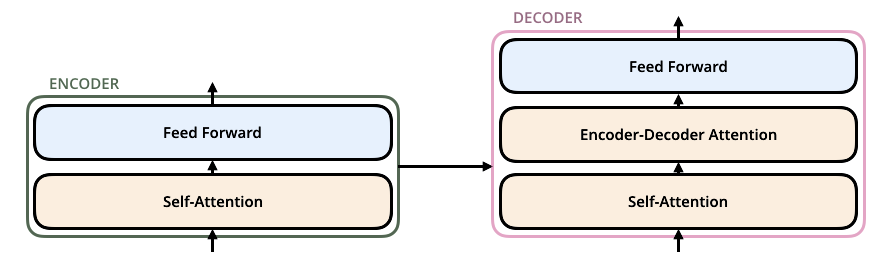
\includegraphics[scale=0.3]{images/encoder_decoder_illustrated_transformer}}
	\caption{البنية الأساسية للمرمز و مفكك الترميز
		داخل المحول
		\textLR{\cite{illustratedTransformer}}}
	\label{fig:enc_dec}
\end{figure}

\begin{figure}[h!]
	\centerline{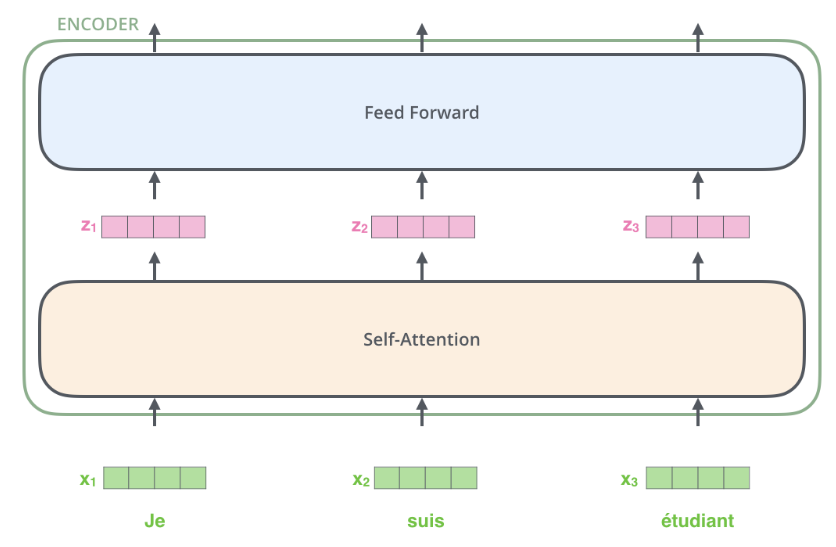
\includegraphics[scale=0.3]{images/position_wise_illustrated_transformer}}
	\caption{\textRL{تطبيق التوابع داخل المحول لكل عنصر دخل بشكل تفرعي}
	\textLR{\cite{illustratedTransformer}}}
	\label{fig:positionWise}
\end{figure}
 
\subsection{مفكك الترميز}
يوضح الشكلان
\ref{fig:Transformer}،\ref{fig:enc_dec}
بنية مفكك الترميز،
وكما في المرمز فإنه يتكون بالإضافة إلى كتلتي الانتباه الذاتي والشبكة الأمامية فإنه أيضاً يحتوي على كتلة إضافية وهي الانتباه التقاطعي متعدد الرؤوس.
%\ref{MCHA}
%دخل هذا التابع هو دخل مفكك الترميز بعد إضافة الترميز المكاني، بحيث يكون %دخل مفكك الترميز  هو خرج آخر طبقة في المرمز.
في خوارزمية المحول الأساسية
\textLR{\cite{Vaswani17}}
يكون دخل مفكك الترميز  هو خرج آخر طبقة في المرمز.
\subsection{ترميز المعلومات المكانية
\textLR{positional encoding\label{PE}}}
كما ذكرنا سابقاً فإن معظم نماذج
\textLR{seq2seq}
قبل ظهور نموذج المحول
\textLR{\cite{Vaswani17}}
كانت تستخدم الشبكات العودية
\textLR{RNN}
مع 
\textLR{LSTM}،
وهذا النوع من الشبكات يحافظ على المعلومات المكانية النسبية لعناصر سلسلة الدخل،  لكن الاستغناء عن شبكات 
\textLR{RNN}
والاستعانة فقط بتوابع الانتباه لمعالجة السلاسل يفقد المعلومات المكانية.
\newline
لمعالجة هذه المشكلة كان من اللازم إدخال المعلومات المكانية للسلسلة بشكل ما، هنا تم طرح طريقة ترميز الموقع لإضافة المعلومات المكانية لكل عنصر من عناصر السلسلة وذلك بإضافة قيم مستخرجة من توابع بترددات مختلفة كما في المعادلات 
\ref{eq:PE}
\textLR{\cite{Vaswani17}}.
\begin{equation}
\begin{split}
	&PE_{(pos,2i)} = sin(pos/1000^{2i/d_{model}})\\
	&PE_{(pos,2i+1)} = cos(pos/1000^{2i/d_{model}})\\
\end{split}
\label{eq:PE}
\end{equation}
حيث 
\textLR{pos}
موقع عنصر الدخل من السلسلة، و
$i$
هو البعد 
\textLR{dimension}.
ويتم إضافة قيم هذه التوابع إلى دخل كل من المرمز ومفكك الترميز.
\newline
اختبرت العديد من الأبحاث طرق الترميز المكاني، فأبسط الأشكال هي إسناد رقم طبيعي أو حقيقي مميز أو عدد ضمن المجال
$[0,1]$
 إلى كل عنصر من عناصر السلسلة
\textLR{\cite{web:PE}}.
\newline
لكن هذه الطرق البسيطة لم تحسن النتائج لأنها لم تستطع أن تجعل النموذج يلتقط معلومات المواقع بين العناصر.
هنا اقترح البحث 
\textLR{\cite{Vaswani17}}
أن يكون ترميز الموقع تابع جيبي كما في المعادلات 
\ref{eq:PE}،
إذ يمكن اعتبار  سلسلة الدخل سلسلة زمنية وكل عنصر هو خرج السلسلة عند خطوة زمنية معينة
\textLR{\cite{web:PE}}،
هذه الطريقة في التفكير ساعدت النموذج على كشف معلومات الموقع النسبية بين العناصر.
 
في الملاحق المستخدم في بحثنا
\textLR{SwinTrack\cite{swinTrack}\ref{section:swintrack}}
تم استخدام 
\textLR{untied PE \cite{untiedPE}}
مع بارامترات قابلة للتدريب.
\subsection{تابع الانتباه\label{att}}
كما ذكرنا في الفقرات السابقة فإن تابع الانتباه هو الجزء الأساسي في نموذج المحول، لذلك وجب شرحه بشيء من التفصيل في الفقرة الحالية، إذ سنشرح عن التابع بشكل عام وعن مفهوم الانتباه، ثم سنشرح عن طريقة استخدامه في نموذج المحول.
\subsubsection{الفكرة العامة لتابع الانتباه الذاتي 
\textLR{self-attention}
\label{section:att_example}
}
لتبسيط شرح مفهوم تابع الانتباه الذاتي سنقوم بالاستعانة بمثال بسيط عن الترجمة، إذ يمكن إسقاط هذا المثال على مجالات أخرى كالرؤية الحاسوبية، وذلك باعتبار $"$الكلمة$"$ مقابلة لـ $"$البكسل$"$ أو $"$مجموعة من البكسلات$"$.
\newline
لنأخذ كمثال جملة 
\textLR{Bank of a river}.
\newline
بداية نحول كل كلمة إلى تمثيل رقمي ندعوه بالـ
\textLR{token}
عبر
\textLR{word embedding}.
هناك العديد من الخوارزميات المدربة مسبقاً لهذا الغرض، بحيث تكون الكلمات المتشابهة بالمعنى $"$متشابهة$"$ أيضاً بالتمثيل الرقمي (أي أن الجداء السلمي لها قيمة قريبة من الواحد). عندها يمكن تمثيل الجملة السابقة كما يلي:
\newline
\textLR{Bank of a river}
\newline
$[word_1, word_2, word_3, word_4]$
\newline
بعد تحويل الـ
\textLR{embedding}
\newline
$X = [x_1,x_2,x_3,x_4]$
\newline
كما ذكرنا سابقاً هدف الانتباه هو تعديل شعاع الـ
\textLR{embedding}
ليناسب السياق. سنشرح فيما يلي كيف يتم ذلك.
\newline
أولاً نحسب التشابه بين كل كلمة في الجملة مع كل كلمات الجملة وذلك عن طريق الجداء السلمي 
\textLR{dot-product}
كما في المعادلات
\ref{eq:att_dot_product}.
\begin{equation}
\begin{split}
&s_{11} = x_1.x_1\\
&s_{12} = x_1.x_2\\
&\text{...}\\
&s_{ij} = x_i.x_j\\
\end{split}
\label{eq:att_dot_product}
\end{equation}
نطبق
\textLR{softmax}
لجعل قيم التشابه ضمن المجال
$[0,1]$
بحيث يكون التشابه بين الكلمة $i$ وكامل الجملة كما في المعادلة 
\ref{eq:att_softmax}.
\begin{equation}
score_{i1},score_{i2},... = softmax(s_{i1},s_{i2},..)
\label{eq:att_softmax}
\end{equation}
من خلال استخدام تابع الانتباه يتم تعديل تمثيل الكلمة $x_i$  بحسب التشابه بينها وبين كلمات الجملة أي بحسب قيم الـ $score_{ij}$، فيكون التمثيل المعدل كما في المعادلة 
\ref{eq:att_fin}>
\begin{equation}
x_{i_{new}} = score_{i1}*x_1+score_{i2}*x_2+...
\label{eq:att_fin}
\end{equation}
وبهذه الطريقة يتغير تمثيل كل كلمة بحسب السياق الكامل للجملة. 
\newline
يستخدم نموذج المحول تابع انتباه مع أشعة تسمى بـ
\textLR{Query ,Keys,Values}،
هذه التسمية مستوحاة من أنظمة الاسترجاع
\textLR{retrieval systems}.
بشكل عام يكون لتابع الانتباه  شعاعا دخل
$X_1,X_2$،
يولد
$X_2$
الـ
\textLR{Query}،
ويولد
$X_1$
كل من الـ
\textLR{Key,Value}،
وذلك باستخدام مصفوفات
$W_q,W_v,W_k$
عناصرها أوزان قابلة للتدريب كما في المعادلات 
\ref{eq:att_mat}.
\begin{equation}
\begin{split}
&Q = X_2 W_q\\
&K = X_1 W_k\\
&V = X_1 W_v\\
\end{split}
\label{eq:att_mat}
\end{equation}
بالنسبة لتابع الانتباه الذاتي يكون
$X_1 = X_2$.
أما في الانتباه التقاطعي الذي سنذكره لاحقاً في الفقرة
\ref{section:attention}
فإن
$X_1$
مصدرها خرج المرمز، أما
$X_2$
فمصدرها مفكك الترميز.
\subsubsection{الانتباه\label{section:attention}}
 هناك نوعان من الانتباه في نموذج المحول، الانتباه الذاتي
\textLR{self-attention}،
والانتباه التقاطعي
\textLR{cross-attention}.
بالنسبة لتابع الانتباه الذاتي له ثلاث مداخل وهي
\textLR{Q query,K key,V value}،
هذه المصفوفات ناتجة عن ضرب مصفوفة الدخل
$X$
في كل طبقة مرمز بمصفوفات
$W_q,W_v,W_k$
 بالتسلسل كما في المعادلات
\ref{eq:att_mat}،
وعناصر هذه المصفوفات هي أوزان تحدد قيمها أثناء التدريب.
\newline
يمكن أيضاً أن نعبر عن تابع الانتباه باستخدام مصفوفات
$Q,K,V$
بالمعادلة
\ref{eq:att}
\textLR{\cite{Vaswani17}}
وكما يوضحه الشكل 
\ref{fig:att_dot_prod}.
\begin{equation}
\begin{split}
Attention(Q,K,V) = softmax(\frac{QK^T}{\sqrt{d_k}})V
\label{eq:att}
\end{split}
\end{equation}
\begin{figure}[h!]
\centerline{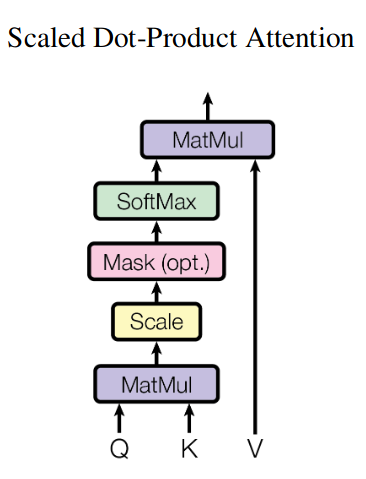
\includegraphics[scale=0.4]{images/att_dot_prod.png}}
\caption{\textRL{حساب تابع الانتباه عن طريق الجداء السلمي المقيس}
\textLR{\cite{Vaswani17}}}
\label{fig:att_dot_prod}
\end{figure}
إذ نلاحظ أن تابع الانتباه يتكون من مرحلتين، المرحلة الأولى هي حساب الـ
\textLR{score}
\begin{equation}
score(Q,K) = softmax(\frac{QK^T}{\sqrt{d_k}})
\end{equation}
والمرحلة الثانية هي تعديل مصفوفة القيم
$V$
بحسب قيم الـ
\textLR{score}.
إن دخل وخرج تابع الانتباه في المعادلة
\ref{eq:att}
هو عبارة عن مصفوفات.
\newline
ولفهم كيف يؤثر هذا التابع على كل شعاع
\textLR{token}
من أشعة الدخل،
نحسب الانتباه الذاتي للشعاع
$x_i$
من مصفوفة الدخل 
$X$.
بداية نحسب كل من قيمة
$k_i,q_i,v_i$
بحسب المعادلات
\ref{eq:att_mat_i}.
\begin{equation}
\begin{split}
&k_i = x_i W_k\\
&q_i = x_i W_q\\
&v_i = x_i W_v\\
\end{split}
\label{eq:att_mat_i}
\end{equation}
نحسب الجداء السلمي بين
$q_i$
وبين كل عنصر من عناصر المصفوفة
$K$ 
كما في المعادلات
\ref{eq:att_mat_i2}.
كما نعلم بأن الجداء السلمي يقيس مدى التشابه بين الشعاع
$q_i$
وبين أشعة المصفوفة
$K$.
ومن ثم نقيّس هذه القيم بتقسيمها على
$\sqrt{d_k}$،
حيث 
$d_k$
هو بعد النموذج 
%كما في الجدول 
%\ref{table:transformer_sympols}
أي بعد شعاع الدخل.
وقد وجد أن التقسيم على هذه القيمة جعل المشتق أكثر استقراراً
\textLR{\cite{illustratedTransformer}}.
ومن ثم بحساب الـ
\textLR{softmax}
والذي يضمن أن تكون القيم مقيسة بين
$[0,1]$،
خرج الـ
\textLR{softmax}
ندعوه بالـ
\textLR{score}.
 وقيم الـ
\textLR{score}
تحدد العناصر التي يجب التركيز عليها أثناء حساب خرج المرمز.
\begin{equation}
	\begin{split}
	&s_{11} = q_1.k_1\\
	&s_{12} = q_1.k_2\\
	&...\\
	&s_{1d} = q_1.k_d\\
	&score =score_1,score_2,..= softmax(\frac{s_{11}}{\sqrt{d_k}},\frac{s_{12}}{\sqrt{d_k}},...)\\
	\end{split}
	\label{eq:att_mat_i2}
\end{equation}
يوضح الشكل 
\ref{fig:att_score}
المرحلة الأولى من تابع الانتباه
\begin{figure}[H]
	\centerline{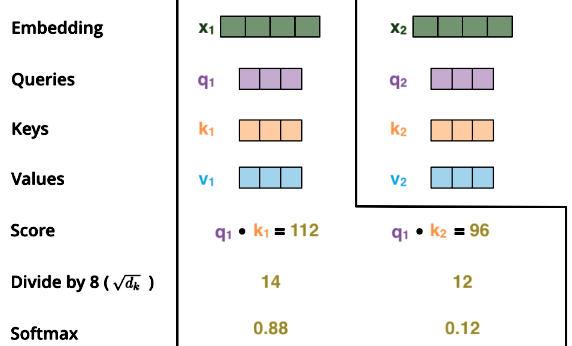
\includegraphics[scale=0.4]{images/att_score}}
	\caption{\textRL{ مثال رقمي عن حساب الـ}
		\textLR{score}
		\textRL{لتابع الانتباه عن طريق الجداء السلمي}
		\textLR{\cite{IllustratedAttention}}}
	\label{fig:att_score}
\end{figure}
المرحلة الثانية هي بحساب الخرج النهائي لتابع الانتباه
$z_1$
 وذلك بالتركيز على قيم 
$V$
بحسب التشابه بين 
$q,K$
كما في المعادلة 
\ref{eq:att_mat_fin}،
وكما يوضحه الشكل 
\ref{fig:att_output}،
وبالمثل نحسب
$z_2,z_3,...$.
\begin{equation}
z_1 = score_1.v_1 + score_2.v_2+....
\label{eq:att_mat_fin}
\end{equation}
\begin{figure}[H]
	\centerline{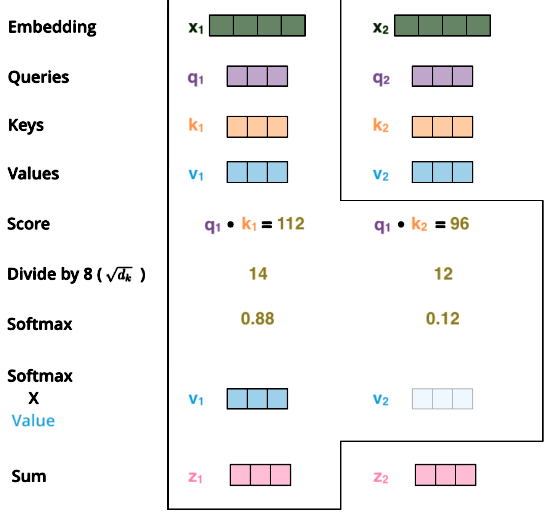
\includegraphics[scale=0.4]{images/attention_output.png}}
	\caption{\textRL{شكل توضيحي لحساب الانتباه من أجل كل عنصر دخل}
		\textLR{\cite{illustratedTransformer}}}
	\label{fig:att_output}
\end{figure}
%ونلاحظ من حساب الخرج أننا نقوم بالتركيز على قيم
%$V$
%بحسب التشابه بين 
%$q,K$.
%وبالمثل نحسب
%$z_2,z_3,...$.
%ويمكننا أن نحول الحساب إلى جداء مصفوفات مباشرة كما في معادلة حساب الانتباه 
%\ref{eq:att}.
\subsubsection{ الانتباه المتعدد الرؤوس
\textLR{Multi-head attention MHA}
}
إحدى الإضافات المهمة في نموذج المحول هي استخدام الانتباه المتعدد الرؤوس. وفيها يحسب الانتباه عدة مرات بحسب عدد الرؤوس
$h$
بشكل تفرعي، كما يوضحه الشكل
\ref{fig:MHA}
\begin{figure}[h!]
	\centerline{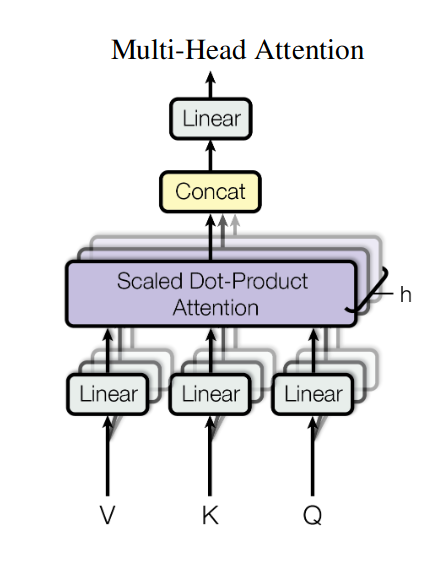
\includegraphics[scale=0.4]{images/MHA.png}}
	\caption{\textRL{الانتباه متعدد الرؤوس}
		\textLR{\cite{Vaswani17}}}
	\label{fig:MHA}
\end{figure}
يتم سَلسَلة (ضم)
\textLR{concatenate}
 خرج الرؤوس ضمن سلسلة واحدة، وعبر شبكة خطية من طبقة واحدة يتم تحويل أبعاد السلسلة إلى أبعاد النموذج من جديد عبر استخدام مصفوفة  الخرج
$W_0$.
\begin{equation}
\begin{split}
&MultiHead(Q,K,V) = Concat(head_1,...,head_H)W^O\\
&\text{\textLR{where  }} head_i = Attention(QW_i^Q,KW_i^K,VW_i^W)\\
\end{split}
\end{equation}
وبحسب
\textLR{\cite{Vaswani17}}،
فإن حساب الانتباه من أجل عدة رؤوس يسمح للنموذج بنمذجة معلومات السمات من مواقع مختلفة بشكل مشترك للرؤوس، وبعبارة أخرى معالجة سمات الدخل في عدة رؤوس يسمح لكل رأس أو نموذج انتباه بالتركيز على مجموعة معينة من السمات وهذا ما يفسر تحسن الأداء
\textLR{\cite{web:attention in cv}}.
في النموذج الأساسي
\textLR{\cite{Vaswani17}}
استخدمت توابع انتباه بعدد الرؤوس
$h = 8$
\subsubsection{الانتباه التقاطعي
\textLR{cross-attention}\label{MCHA}}
بالإضافة إلى حساب الانتباه الذاتي في مفكك الترميز
بين مداخله، فإنه أيضاً يُحسب
الانتباه بين المرمز ومفكك الترميز. نستخلص من خرج الطبقة الأخيرة من المرمز كل من الأشعة 
$V,K$،
ومن دخل طبقة مفكك الترميز نستخلص الشعاع 
$Q$.
\subsubsection{أنواع توابع الانتباه
\textLR{\cite{IllustratedAttention}}}
هناك عدة أنواع من التوابع لحساب
\textLR{score}
 الانتباه كما هو موضح في الشكل
\textLR{\ref{fig:att_types}}
 \begin{figure}[h!]
 	\centerline{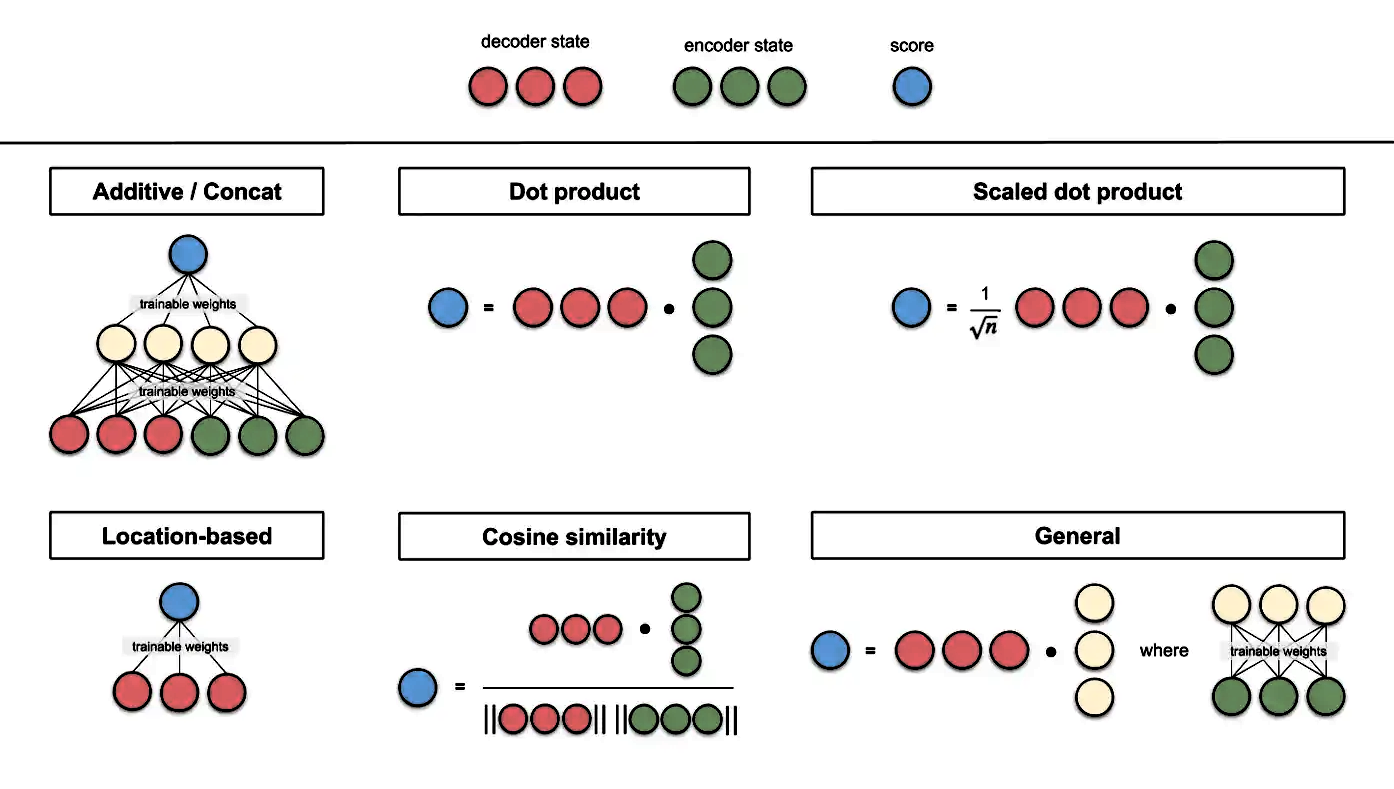
\includegraphics[width=\textwidth]{images/attention_types}}
 	\caption{\textRL{أنواع توابع الانتباه}
 	\textLR{\cite{IllustratedAttention}}}
 	\label{fig:att_types}
 \end{figure}

\begin{itemize}
	\item الانتباه الجمعي 
	$score(A,B) = v_\alpha^T tanh(W_a[A;B])$
	\item
	انتباه الجداء السلمي 
	$score(A,B) = A^TB$
	\item
	انتباه الجداء السلمي المقيس
	$score(A,B) = \frac{A^TB}{\sqrt{ns}}$
	وهو النوع المستخدم في نموذج المحول 
	\textLR{\cite{Vaswani17}}،
	حيث
	$n$
	هي بعد الشعاع
	$B$.
	\item الانتباه المعتمد على المحتوى
	$score(A,B) = cosine[A,B] = \frac{A.B^T}{||A||.||B||}$ 
	
	\item
	الانتباه العام
	$score(A,B) = A^TW_aB$


	
\end{itemize}
\section{المحول في الرؤية الحاسوبية}
في هذه الفقرة سنذكر استخدامات نموذج المحول في مجال الرؤية الصنعية، إذ بسبب النجاح الذي حققه المحول في تطبيقات معالجة اللغات الطبيعية، فقد استخدم في مجالات الرؤية الحاسوبية في السنوات الأخيرة، وقدأعطى نتائج تفوقت على أحدث وأفضل الخوارزميات في هذا المجال بالنسبة للعديد من معايير التقييم في هذا المجال مثل 
\textLR{Imagenet, coco}
وغيرها
\textLR{\cite{ViTsurvey}}.
فقد تم استخدام المحول في مجال توليد
\textLR{\cite{Transgan}}،
تصنيف
\textLR{\cite{ViT}}،
كشف
\textLR{\cite{DETR}}،
وتحسين الصور
\textLR{\cite{Pre-trainedimageTransformer}}،
تصنيف الفيديو
\textLR{\cite{Non-local neural networks}}،
والملاحقة
\textLR{\cite{transformertracker}}،
والذي هو موضوع بحثنا.
\newline
سنتكلم بإيجاز في هذه الفقرة عن النماذج الأولى والأساسية التي استخدمت المحول في مجال الرؤية الصنعية وهي نموذج
\textLR{ViT\cite{ViT}}
ونموذج
\textLR{DETR\cite{DETR}}.
وقد ظهرت بعدها الكثير من النماذج التي اعتمدت على المحول في تطبيقات الرؤية الحاسوبية.
\subsection{المحول والشبكات التلافيفية}
ذكرنا في فقرة سابقة 
\ref{section:transformer}
أن المحول استغنى عن شبكات 
\textLR{RNN}
والتي كانت الأكثر استخداما في مجال معالجة اللغات الطبيعية
\textLR{\cite{Vaswani17}}،
وتحدثنا عن المشكلات التي تعاني منها هذا النوع من الشبكات ذات المعالجة التسلسلية. أما فيما يخص الرؤية الحاسوبية فإن شبكات
\textLR{CNN}
هي الأكثر استخداماً، وهي على العكس من شبكات 
\textLR{RNN}
يمكن بفعالية أن تعالَج بشكل تفرعي باستخدام  
\textLR{GPU}.
ولكن حتى الآن فإن الكثير من الأبحاث لم تستبدل شبكات
\textLR{CNN}
بنموذج المحول بشكل كلي بالرغم من تفوق المحول في الأداء عند تدريبه على معطيات كافية. والسبب في ذلك يعود إلى محاسن شبكات 
\textLR{CNN}
من حيث المحلية
\textLR{locality}،
أي أخد البكسلات المجاورة بعين الاعتبار عند المعالجة كما سنذكر لاحقاً.
\subsubsection{ميزات الشبكات التلافيفية}
\begin{itemize}
\item
غير متغيرة مع الانسحاب
\item
تأخذ العمليات الحسابية في هذه الشبكات المناطق المحلية بعين الاعتبار، فبالتالي السمات المستخرجة منها حساسة محلياً وتحمل معلومات مكانية بشكل أكبر من المحول.
\item
وبسبب هذه الميزة وهي المحلية،
فإن
\textLR{CNN}
جيدة لاستخراج السمات من الصورة، ولكن ليست قادرة على نمذجة العلاقات أو الارتباطات بين هذه السمات، وبالتالي تفتقر إلى الفهم العام للصورة. أما بالنسبة للمحول فإن نقطة قوته هي القدرة على فهم السياق العام
\textLR{\cite{TransformerCV}}،
والنمذجة بشكل
\textLR{global}
أي نمذجة العلاقات الطويلة الأمد بين السمات
\textLR{long-range dependencies}
\textLR{\cite{Swin Transformer V1 and V2}}.
\end{itemize}
بعض الأعمال استخدمت المحول في مجال الرؤية الحاسوبية وقد أعطت نتائج تفوقت على الخوارزميات الرائدة في هذا المجال عند وجود عدد كافي من معطيات التدريب، وذلك بالاعتماد فقط على توابع الانتباه ودون أي استخدام للشبكات التلافيفية 
\textLR{\cite{ViT}}،
بالرغم من أن هذه النماذج لها بنية أبسط، وتستهلك زمن تدريب أقل مقارنة بنماذج الشبكات التلافيفية
\textLR{\cite{TransformerCV}}.
\subsection{المحول في مجال التصنيف}
ظهرت العديد من خوارزميات التصنيف التي تستخدم المحول في السنوات الأخيرة، بعضها قد حسن الخوارزميات المعتمدة على الشبكات التلافيفية بإضافة أجزاء من المحول إليها، وذلك كونه ينمذج الترابطات الطويلة الأمد، مثل
\textLR{VT\cite{VT}}،
\textLR{BotNet\cite{BotNet}}.
وكون البنية الأصلية للمحول 
\textLR{\cite{Vaswani17}}
تهمل المعلومات المحلية، لذلك كان هنالك العديد من التحسينات على بنية
\textLR{ViT\cite{ViT}}،
من هذه التحسينات إضافة أجزاء من الشبكات التلافيفية لتحسين المحول، مثل خوارزمية
\textLR{BEiT\cite{BEiT}}،
وخوارزمية 
\textLR{ConViT\cite{ConViT}}.
\newline
وهناك تحسينات أخرى مثل المحول الذي يعتمد على الانتباه المحلي،
هذه الخوارزميات قد أعادت تصميم تجزئة الصورة 
\textLR{patch partition}،
وأعادت تصميم كتل توابع الانتباه بهدف إضافة المعلومات المحلية(المكانية) إلى المحول، دون الاعتماد على الشبكات التلافيفية وذلك مثل خوارزمية 
\textLR{TNT\cite{TNT}}،
\textLR{Volo\cite{Volo}},
و 
\textLR{SwinTransformer\cite{swintransformer}}
والتي سنتحدث عنها في الفقرة
\ref{section:swinTransformer}
كونها الـ
\textLR{backbone}
المستخدم في نموذجنا.
\newline
عدلت العديد من الأبحاث بنية المحول  إلى بنية هرمية وعميقة مثل
\textLR{T2T-ViT\cite{T2T-ViT}}،
\textLR{PVT\cite{PVT}}،
وذلك محاكاة لبنية الشبكات التلافيفية الهرمية والعميقة 
\textLR{\cite{Why Deep Learning Works}}.
\newline
بحسب المقالة
\textLR{\cite{ViTsurvey}}،
والتي تقارن وتصنف أكثر من مئة محول في مجال الرؤية الحاسوبية فإن الأبحاث الحديثة لا تميل إلى استخدام البنية الأصلية للمحول، ولم تستغني عن استخدام الشبكات التلافيفية بشكل كامل، بل العكس من ذلك استخدام البنية الهجينة هو ما يعطي أفضل النتائج، بالرغم من أن المحول يمكن أن يوازي بأداءه الشبكات التلافيفية أو حتى يفوقها في الأداء، ويعود ذلك إلى أن المعلومات المحلية مهمة جداً لتحسين أداء المحول كما في 
\textLR{Volo\cite{Volo}}،
و
\textLR{SwinTransformer\cite{swintransformer}}،
وهما نسخة المحول الأكثر استخداما في الرؤية الحاسوبية.
في هاتين الخوارزميتين تم استخدام خليط من المعلومات العامة 
\textLR{global}
والمعلومات المحلية 
\textLR{local}.
\newline
أما على صعيد تحسين الاجزاء الأخرى من المحول مثل تحسين الترميز المكاني
\textLR{Positional Encoding PE}
فهناك العديد من الأبحاث مثل
\textLR{\cite{Conditional positional encodings for ViT}}،\textLR{\cite{RethinkingPE}}،\textLR{\cite{deeper look at position information in cnns}}. 
أو تحسين بنية
\textLR{MHA}
الانتباه متعدد الرؤوس
\textLR{\cite{Cordonnier}}،
أو تحسين 
\textLR{MLP}
كما في 
\textLR{\cite{Attention is not all you need}}.
\subsection{المحول في مجال الكشف}
أول خوارزمية استخدمت المحول في مجال الكشف هي 
\textLR{DETR\cite{DETR}}،
استخدمت هذه الخوارزمية تمثيل جديد وهو
\textLR{object query}،
وهو أحد مداخل مفكك الترميز،
وهو مجموعة من الأوزان القابلة لتعلم السمات العامة في الصورة. كان هناك العديد من التحسينات على هذه الخوارزمية مثل
\textLR{DeformableDETR\cite{DeformableDETR}}،
و
\textLR{ACT\cite{ACT}}،
كون الخوارزمية الأصلية
\textLR{\cite{DETR}}
تعاني من دقة كشف منخفضة من أجل الأغراض الصغيرة وتأخذ زمن طويل في التدريب.
\newline
هناك العديد من الدراسات التي أعادت تصميم بنية المحول مثل
\textLR{TSP\cite{TSP}},
\textLR{YOLOS\cite{YOLOS}}.
أو باستخدام المحول كـ
\textLR{backbone}
لاستخلاص السمات من الصورة كما في
\textLR{FPT\cite{FPT}}.
\subsection{خوارزمية التصنيف
\textLR{ViT\cite{ViT}}}
هذه الخوارزمية لا تستخدم الشبكات التلافيفية في بنيتها. إذ يتم تقسيم الصورة إلى أقسام عدة
\textLR{patches}،
كل قسم
\textLR{patch}
يعامل معاملة ال 
\textLR{token}
(الكلمة) في المحول الأصلي، أي يتم إدخاله إلى طبقة
\textLR{embedding}
خطية لتحويله إلى شعاع بأبعاد مختلفة.
\newline
عند تدريب هذا النموذج على معطيات تدريب ذات حجم متوسط مثل
\textLR{ImageNet}
كان أداؤه متواضع وأقل من أداء نموذج
\textLR{ResNet\cite{ResNet}}
و بعدد أوزان متقارب. لكن النتائج تغيرت عند تدريبه على معطيات تدريب بحجوم كبيرة ( 
$14$
مليون -
$300$ 
مليون عينة) مثل 
\textLR{ImageNet-21K},
\textLR{JFT-300M}،
عندها أعطى النموذج نتائج تفوقت على الخوارزميات السابقة.
\newline
دخل النموذج الأصلي للمحول هو سلسلة ببعد واحد . للتعامل مع الصورة وللمحافظة على البنية الأساسية للمحول فقد  تم تعديل الصورة
$x\in \mathds{R}^{H\mathsf{x}W\mathsf{x}C}$
وتحويلها إلى سلسلة من الأجزاء المسطحة
$x_p \in  \mathds{R}^{N\mathsf{x}(P^2.C)}$
ذات بعد واحد، وذلك لمحاكاة دخل المحول الأصلي. حيث
$H\mathsf{x}W$
أبعاد الصورة،
$C$
عدد القنوات والتي هي في الغالب
$RGB = 3$،
$P\mathsf{x}P$
أبعاد كل قسم من الصورة
\textLR{patch}،
$N$
 عدد الأقسام أو الأجزاء
$N = \frac{HW}{P^2}$.
\newline
يتم إدخال الشعاع 
$x_p$
إلى طبقة إسقاط خطي أي شبكة عصبونية بطبقة واحدة مع تابع تفعيل خطي، وذلك لتحويل أبعاده إلى 
$(N,D)$
كما في المعادلة
\ref{eq:vit1}.
\begin{equation}
z_0 = [x_{class};X_p^1E;x_p^2E;...;x_p^NE]+E_{pos},	E\in \mathds{R}^{(P^2.C)\mathsf{x}D},E_{pos}\in \mathds{R}^{(N+1)\mathsf{x}D}
\label{eq:vit1}
\end{equation}
\begin{equation}
Z_l^\prime = MSA(LN(z_{l-1})) + z_{l-1},	l = 1 ... L
\label{eq:vit2}
\end{equation}
\begin{equation}
Z_l = MLP(LN(z_l^\prime)) + z_l^\prime,	l = 1 ... L
\label{eq:vit3}
\end{equation}
\begin{equation}
y = LN(z_L^0)
\label{eq:vit4}
\end{equation}
حيث
$D$
هو
\textLR{hyperparameter}
ويمكن تسميته ببعد الـ
\textLR{embedding}.
$E$
هي طبقة الإسقاط الخطي، بعدد بارامترات
$E \in \mathds{R}^{(P^2.C)\mathsf{x}D}$
قابلة للتدريب.
وكما في خوارزمية
\textLR{BERT\cite{BERT}}
فيتم إضافة شعاع من البارامترات ندعوه بالـ
\textLR{class token}
قابل للتدريب بأبعاد
$(1\mathsf{x}D)$،
وهو 
$x_{class}$
في المعادلة 
\ref{eq:vit1}.
 حيث يتم اعتبار أن حالة هذا الشعاع في الخرج النهائي للمحول
$z_L^0$
يمكن تدريبها لتعبر عن صنف الصورة، وذلك بعد تعديل هذا الشعاع بإدخاله إلى شبكة التصنيف
\textLR{classification head}.
$L$
هي عدد طبقات المرمز.
\newline
نضيف إلى هذا الشعاع شعاع ترميز الموقع 
$E_{pos}$
وذلك لإدخال المعلومات المكانية النسبية بين أجزاء الصورة، استخدمت
\textLR{ViT}
ترميز موقع ببعد واحد قياسي.
$Z_0$
هو دخل المحول كما في المعادلة
\ref{eq:vit1}.
\newline
يستخدم
\textLR{ViT}
بنية مرمز مطابقة لبنية المرمز في المحول الأصلي من حيث توابع انتباه متعددة الرؤوس كما في المعادلة 
\ref{eq:vit2}
وشبكة
\textLR{MLP}
كما في المعادلة 
\ref{eq:vit3},
ويتم تطبيق طبقة تقييس قبل كل كتلة، بالإضافة إلى 
\textLR{residual connections\cite{residual}}
بعد كل كتلة. وكما يوضح الشكل
\ref{fig:ViT}

\begin{figure}[h!]
	\centerline{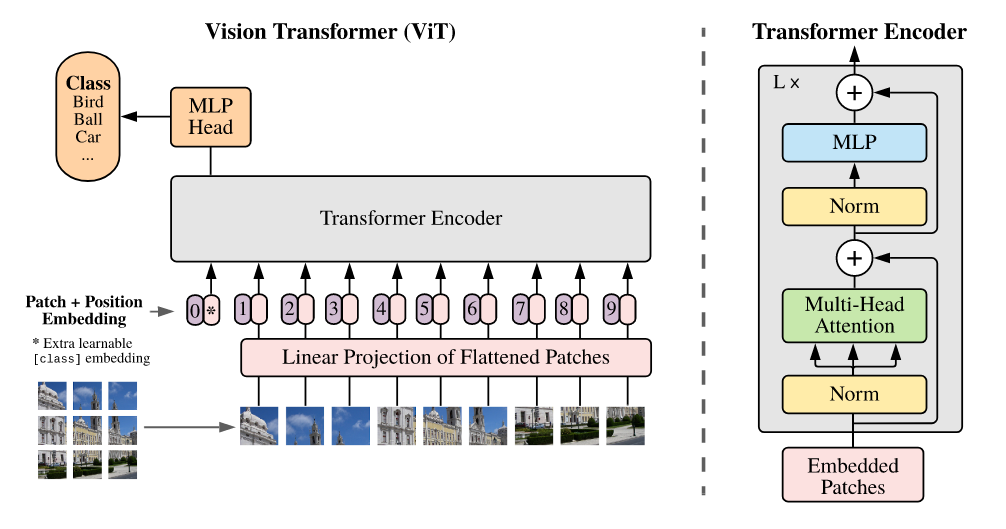
\includegraphics[width=\textwidth]{images/ViT}}
	\caption{
	\textRL{بنية خوارزمية}
	\textLR{ViT}
	\textLR{\cite{ViT}}}
	\label{fig:ViT}
\end{figure}

\subsection{خوارزمية الكشف
	\textLR{DETR\cite{DETR}}
\label{section:detr}}

\begin{figure}[h!]
	\centerline{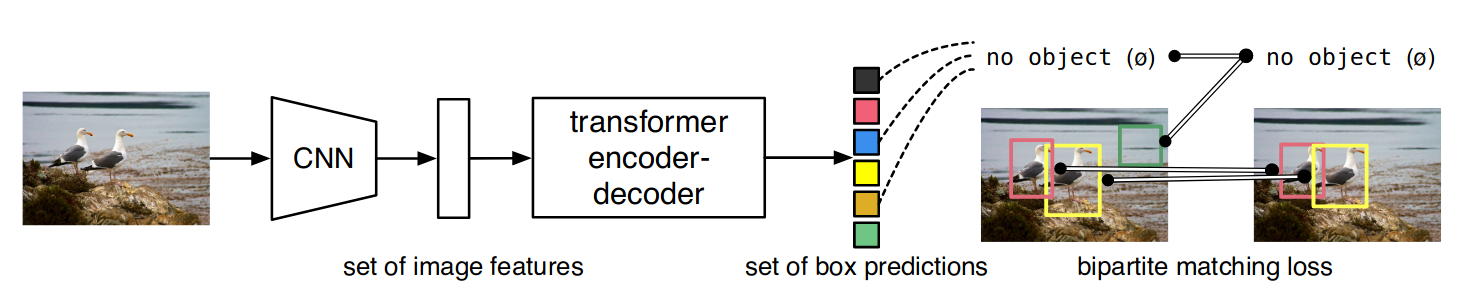
\includegraphics[width=\textwidth]{images/DETR}}
	\caption{\textRL{بنية الكاشف}
	\textLR{DETR}
	\textLR{\cite{DETR}}}
	\label{fig:DETR}
\end{figure}
\selectlanguage{arabic}
كما يوضح الشكل
\ref{fig:DETR}
فإن النموذج يستخدم شبكة تلافيفية كـ
\textLR{backbone}
 لاستخلاص السمات من الصورة التي أبعادها
$x_{img} = \in \mathds{R}^{3\mathsf{x}H_0\mathsf{x}W_0}$،
وأبعاد خريطة السمات بعد الشبكة التلافيفية
$f \in \mathds{R}^{C\mathsf{x}H\mathsf{x}W}$،
حيث
$H,W = \frac{H_0}{32},\frac{W_0}{32}$
و
$C = 2048$.
يتم تخفيض الأبعاد من $C$ إلى  $d$، وتحويل خريطة السمات من بعدين إلى بعد واحد عبر التسطيح
\textLR{flattening}
 فيصبح لدينا أبعاد دخل المرمز
$N\mathsf{x}d$
حيث
$N=H\mathsf{x}W$.
\newline
ونلاحظ أيضا أن الخوارزمية قد اتبعت بنية المحول الأصلي أي بنية مرمز-مفكك ترميز مع فوارق بسيطة مثل دخل مفكك الترميز. في  المحول الأصلي دخل مفكك الترميز هو الخرج في اللحظة الزمنية السابقة، أما في 
\textLR{DETR} 
فهو عبارة بارامترات قابلة للتدريب تدعى
\textLR{object queries}،
تعبر عن ترميز مكاني لكل غرض ويتم فك هذا الترميز عبر مفكك الترميز.
نلاحظ أن كل من الخوارزميتين السابقتين 
\textLR{ViT}
و
\textLR{DETR}
استخدمتا بنية المحول الأصلي مع تعديلات بسيطة. أما بالنسبة  للخوارزمية التي استخدمناها لاستخلاص السمات في نموذجنا وهي محول
\textLR{Swin\cite{swintransformer}}،
والتي سنتحدث عنها في الفقرة التالية فقد عدلت بشكل كبير في بنية المحول.

\subsection{المحول في الملاحقة}
في عام 
$2021$
بدأت تظهر أنظمة ملاحقة تستخدم المحول في بنيتها، سنذكر في هذه الفقرة بعض من تطبيقات المحول في مجال الملاحقة.
\newline
فمثلا استخدمت خوارزمية 
\textLR{TransT\cite{transformertracker}}
الطريقة الموضحة في الشكل 
\ref{fig:TransT}،
بداية تُستخدم شبكة 
\textLR{ResNet-50\cite{ResNet}}
لاستخلاص السمات من صورتي الغرض ومنطقة البحث، ومن ثم تستخدم كتلة انتباه ذاتي لكل من سمات الصورتين، مسماة في الورقة البحثية بـ
\textLR{ECA Ego-Context Augment Modules}
موضحة في المخطط اليسار من الشكل 
\ref{fig:TransT_Modules}.
ويتم دمج هذه السمات عبر كتلة انتباه تقاطعي تدعى بـ
\textLR{CFA Cross-Feature Augment Module}.
يتم الدمج عبر ثلاث مراحل موضحة في الشكل 
\ref{fig:TransT}
\begin{itemize}
	\item
	دمج خرج كتلة 
	\textLR{ECA}
	للغرض باعتبارها 
	\textLR{query}
	 ولمنطقة البحث باعتبارها
 	\textLR{key,value}.
 	\item
 	دمج بتبديل المداخل أي باعتبار سمات الغرض هي 
 	\textLR{key,value}
 	وسمات نافذة البحث هي 
	\textLR{query}.
 	\item
 	دمج الخرجين السابقين ضمن كتلة 
	\textLR{ECA}
	ثالثة.
\end{itemize}
مع إضافة ترميز مكاني إلى كل من 
\textLR{key,query}
في كل كتلة.
\newline

\begin{figure}[!h]
	\centerline{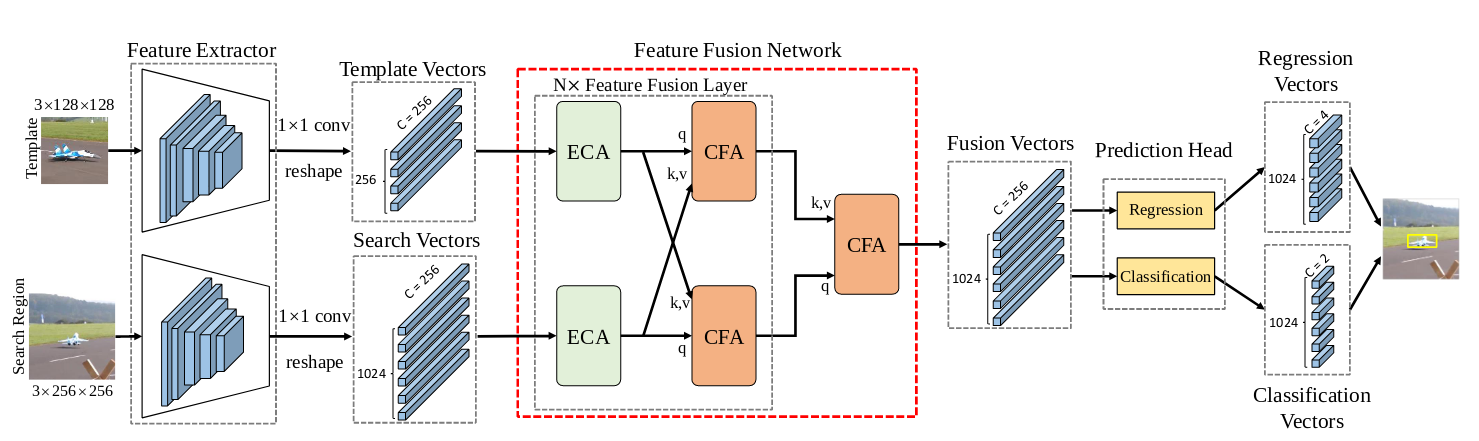
\includegraphics[width=\textwidth]{images/TransT}}
	\caption{
		\textRL{بنية خوارزمية الملاحقة}
		\textLR{TransT}
		\textLR{\cite{transformertracker}}}
	\label{fig:TransT}
\end{figure}

\begin{figure}[!h]
	\centerline{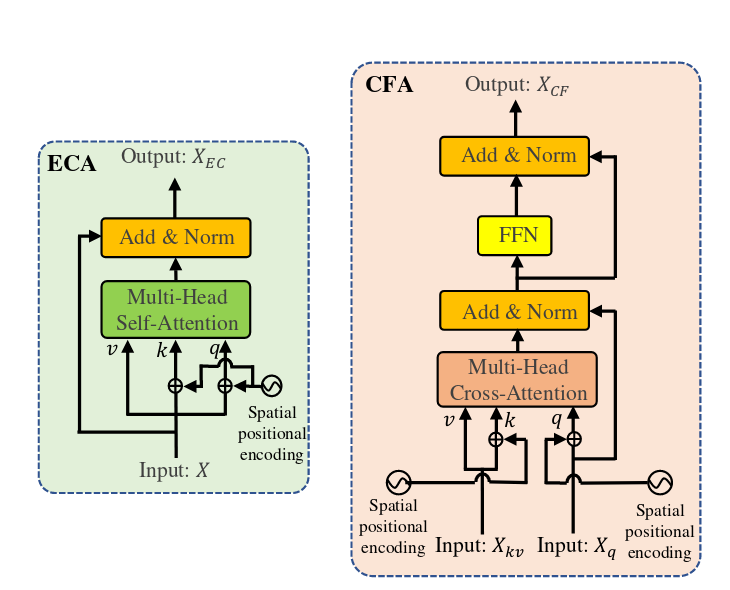
\includegraphics[scale=0.4]{images/TransT_ECA_CFA.png}}
	\caption{
		\textRL{بنية خوارزمية الملاحقة}
		\textLR{TransT}
		\textLR{\cite{transformertracker}}}
	\label{fig:TransT_Modules}
\end{figure}
كما أن خوارزمية الملاحقة
\textLR{TrTr\cite{TrTr}}
تستخدم بنية شبيهة ببنية المحول الأصلي كما يوضح الشكل 
\ref{fig:TrTr}،
بحيث يكون دخل المرمز هو سمات صورة الغرض الإبتدائية، ويطبق الانتباه الذاتي للتركيز على السمات المهمة. بينما يكون دخل مفكك الترميز هو سمات نافذة البحث ويطبق عليها تابع انتباه ذاتي، والدخل الثاني هو خرج المرمز (سمات الغرض المعدلة)، ويتم تطبيق تابع الانتباه التقاطعي بين الدخلين.
\begin{figure}[!h]
	\centerline{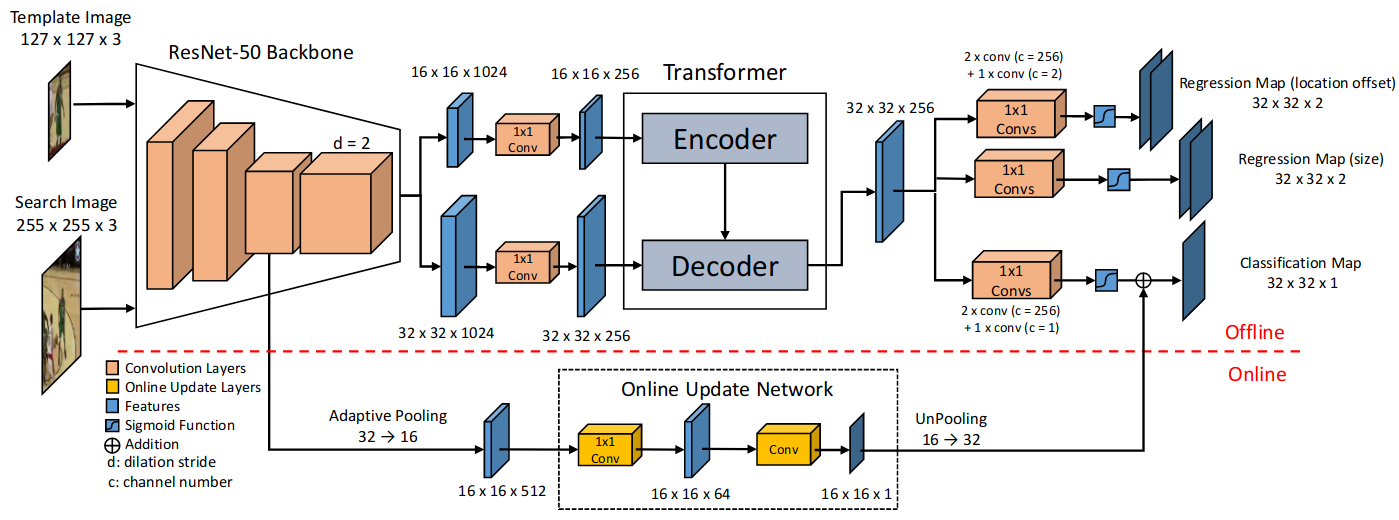
\includegraphics[width=\textwidth]{images/TrTr.png}}
	\caption{\textRL{بنية خوارزمية الملاحقة}
	\textLR{\cite{TrTr}}
	\textLR{TrTr}}
	\label{fig:TrTr}
\end{figure}
\newline
بالإضافة إلى خوارزميتي الملاحقة السابقتين فهناك خوارزمية الملاحقة 
\textLR{STARK\cite{Stark}},
وخوارزمية الملاحقة 
\textLR{SwinTrack\cite{swinTrack}}،
واللتان سيتم شرحهما بالتفصيل في الفصل القادم.
%وقد تم الاعتماد عليهما في البحث، وسيتم شرحهما بالتفصيل في الفصل القادم.
ويجب أن نلاحظ بمقارنة الخوارزميات الأربعة السابقة ببعضها بأن كل من 
\textLR{TransT\cite{transformertracker}}
و
\textLR{TrTr\cite{TrTr}}
تقوم بمعالجة سمات الغرض وسمات نافذة البحث على حدة ضمن توابع الانتباه، بينما في خوارزميات الملاحقة 
\textLR{SwinTrack\cite{swinTrack}}
و
\textLR{STARK\cite{Stark}}
كما سنرى لاحقاً،
فإنها تقوم بضم أشعة السمات للصورتين ضمن شعاع واحد، وتعتبره كدخل للمرمز.
\newline
هذا فيما يتعلق بخوارزميات الملاحقة لغرض واحد والتي تستخدم نموذج المحول ضمن بنيتها، وبمقارنة هذه الخوارزميات بسابقتها والتي لا تستخدم المحول، فنلاحظ كما يوضح الشكل
\ref{fig:comapre}،
والذي يقارن عدة خوارزميات ملاحقة حديثة من ناحية الأداء والسرعة على مجموعة المعطيات الخاصة بالملاحقة 
\textLR{LaSOT\cite{Lasot}}،
بأن خوارزميات الملاحقة التي تستخدم المحول حققت أفضل أداء وسرعة مقارنةً بغيرها من الخوارزميات، وهذا ماشجعنا على اعتمادها في البحث.
وبمقارنة الخوارزميات الأربعة السابقة بالنسبة لبعضها فنلاحظ من الجدول 
\ref{table:compare__trans_trackers}،
والذي يقارن هذه الخوارزميات من أجل مجموعة المعطيات 
\textLR{LaSOT\cite{Lasot}}،
بأن أفضل أداء حققته خوارزمية 
\textLR{SwinTrack\cite{swinTrack}}، 
يليها خوارزمية 
\textLR{STARK\cite{Stark}}،
وبسبب تفوق خوارزمية 
\textLR{SwinTrack\cite{swinTrack}}
في الأداء والسرعة، قررنا أن نعتمدها في بحثنا.
\vspace{-5.0mm}
\begin{figure}[H]
\centerline{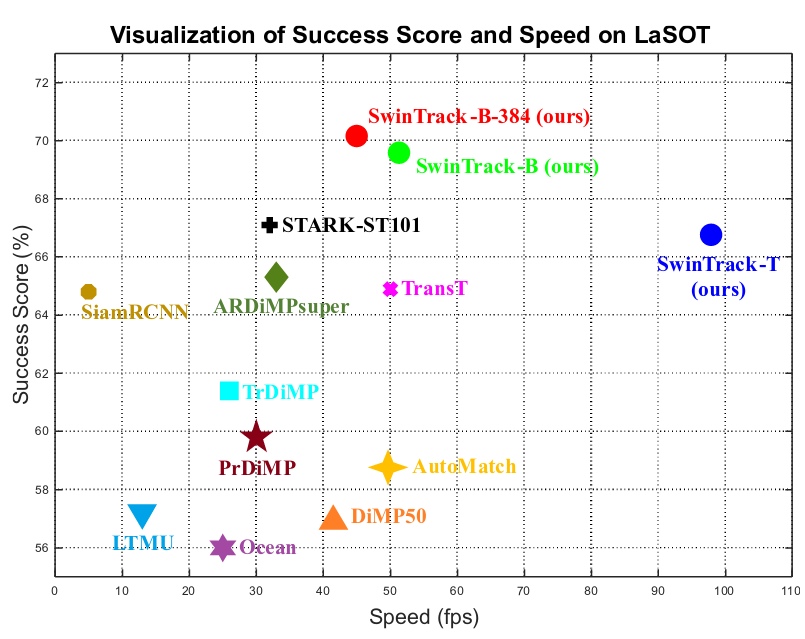
\includegraphics[width=0.6\textwidth]{images/transformerInTrackingComapre.png}}
	\caption{\textRL{
			مقارنة بين بعض الخوارزميات التي تستخدم المحول مع خوارزميات
	}}
	\label{fig:comapre}
\end{figure}
\vspace{-7.0mm}
\centerline{\textRL{
		الملاحقة الأخرى  من ناحية السرعة و الأداء على مجموعة المعطيات
			 \textLR{LaSOT\cite{Lasot}}
		\textLR{\cite{swinTrack}}
}}	

%\begin{figure}[!h]
%	\centerline{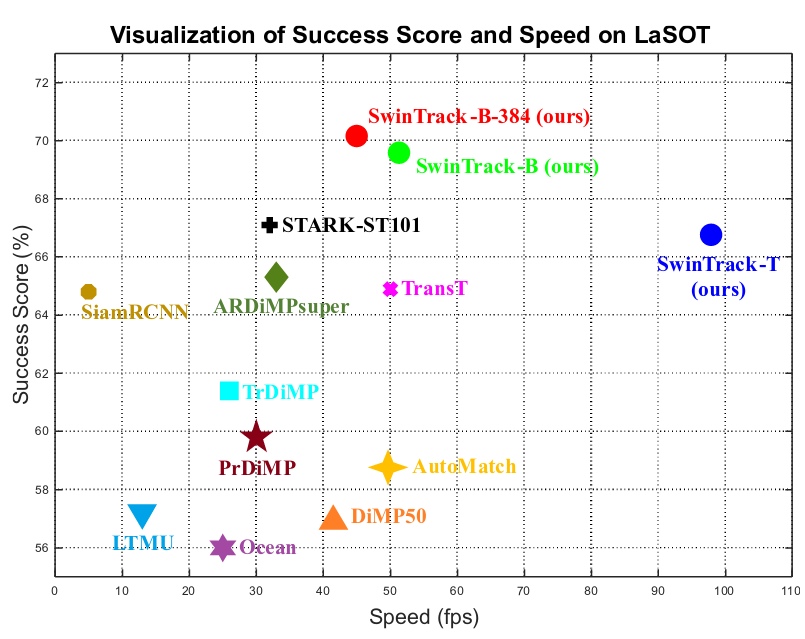
\includegraphics[width=0.6\textwidth]{images/transformerInTrackingComapre.png}}
%	\caption{
%		\textRL{مقارنة بين بعض الخوارزميات التي تستخدم المحول مع خوارزميات الملاحقة الأخرى
%			 من ناحية السرعة و الأداء على مجموعة المعطيات}
%		 \textLR{LaSOT\cite{Lasot}}
%		\textLR{\cite{swinTrack}}
%		}
%	\label{fig:comapre}
%\end{figure}

\begin{table}[H]
	\centering
	\begin{tabular}{c c c c c c c} 
		\hline
		\textLR{Tracker} & \textLR{AUC}\% & \textLR{Normalized Precision} & \textLR{Precision}&\textLR{Year}\\ [0.5ex] 
		\hline\hline
		\textLR{SwinTrack-B-384} &$70.2$&$78.4$&$75.3$&$2021$\\
		\textLR{STARK} & $67.1$ & $77.0$ &&$2021$\\ 
		\textLR{TransT} &$64.9$ & $73.8$ & $69.0$&$2021$\\
		\textLR{TrTr} & $55.1$ &&&$2021$&\\[1ex] 
		\hline
	\end{tabular}
	\caption{
		\textRL{مقارنة بين خوارزميات الملاحقة السابقة}}
	\label{table:compare__trans_trackers}
\end{table}
\vspace{-8.0mm}
\centerline{\textRL{
		\textRL{من أجل معطيات التدريب}
\textLR{LaSOT\cite{Lasot}}	
}}	
أما فيما يتعلق بالملاحقة لعدة أغراض فهناك خوارزمية 
\textLR{TrackFormer\cite{TrackFormer}}
والتي استخدمت بنية محول مشابهة لخوارزمية
\textLR{TrTr\cite{TrTr}},
بينما استخدمت خوارزمية
\textLR{TransTrack\cite{TransTrack}}
سمات الإطار الحالي والإطار السابق كدخل للمرمز مع استخدام كتلتي مفكك ترميز،
دخل مفكك الترميز هو
\textLR{object query} 
قابلة للتدريب، وذلك كما في خوارزمية 
\textLR{DETR\cite{DETR}}
المشروحة في الفقرة 
\ref{section:detr}.
\subsection{المحول 
\textLR{Swin}\label{section:swinTransformer}}
صمم المحول الأصلي ليناسب تطبيقات معالجة اللغات الطبيعية، وبسبب اختلاف هذا المجال عن مجال الرؤية الحاسوبية، ظهرت العديد من الدراسات لتعديل بنية المحول لتتناسب مع مجال الرؤية.
\newline
نذكر بعض الاختلافات بين المجالين
\begin{itemize}
	\item
	في تطبيقات معالجة اللغات الطبيعية فإن الكلمة التي نحولها إلى 
\textLR{token}
	 هي العنصر الأساسي. وكل الـ
\textLR{tokens}
لها نفس الحجم، أما بالنسبة للتطبيقات الرؤية الحاسوبية فإن الأغراض في الصورة أو العناصر المرئية
\textLR{visual elements}
لها حجوم ومقاييس
\textLR{scales}
مختلفة. بعض خوارزميات الكشف قد عالجت مشكلة اختلاف مقاييس الأغراض مثل
\textLR{\cite{Feature pyramid networks for object detection}},
\textLR{\cite{An analysis of scale invariance in object detection}}.
\item
العدد الكبير للبكسلات في الصورة مقارنة بعدد الكلمات في الجملة، وهذا ما يجعل المحول الأصلي ذا تعقيد حسابي كبير من أجل المهمات التي تتطلب معالجة على مستوى البكسل مثل 
\textLR{semantic segmentation}،
أو من أجل الصور ذات الحجوم الكبيرة، حيث يكون التعقيد الحسابي للانتباه الذاتي متناسب بشكل تربيعي مع حجم الصورة.
\end{itemize}
\subsubsection{إشكالية نموذج
\textLR{ViT\cite{ViT}}
ونموذج المحول الأصلي 
\textLR{\cite{Vaswani17}}}
بالرغم أن خوارزمية
\textLR{ViT\cite{ViT}}
لم تعدل على بنية المرمز الأصلي للمحول، إذ أنها فقط جزأت الصورة إلى
$16 \mathsf{x} 16$
جزء 
\textLR{patch}،
إلا أنها تفوقت على أفضل المصنفات حين تم تدريبها على معطيات تدريب كافية 
\textLR{JFT-300M}،
لكن الـ 
\textLR{tokens}
في
\textLR{ViT}
كان لها حجم ومقياس ثابت، وهذا كما ذكرنا في الفقرة السابقة، غير مناسب لأغراض الرؤية الحاسوبية.
المشكلة الأخرى عندما تكون صورة الدخل ذات دقة عالية يزداد التعقيد الحسابي بشكل تربيعي مع زيادة حجم الصورة. وأيضا كل من
\textLR{ViT} 
والنموذج الأصلي
\textLR{\cite{Vaswani17}} 
غير مناسب للتطبيقات التي تحتاج معالجة على مستوى البكسل بسبب التعقيد الحسابي العالي، إذ يتم حساب تابع الانتباه بين الـ
\textLR{tokens}
كلها.
\subsubsection{نموذج
\textLR{Swin}}
كما ذكرنا فإن محول
\textLR{Swin}
هو النموذج المستخدم لاستخراج السمات، وسنبين في هذه الفقرة اختلافه عن المحول الأصلي، وسبب تفوقه من ناحية الأداء والسرعة، وهذا ماجعله مناسب لبحثنا كوننا نهتم بتطبيقات الزمن الحقيقي.
\newline
نموذج محول 
\textLR{Swin}
اختصار لـ
\textLR{Shifted Windows Transformer}،
أي نموذج محول مع نوافذ مزاحة،
وهو نموذج هرمي
\textLR{hierarchical}،
إذ يسمح بالنمذجة من أجل مقاييس متنوعة. بالإضافة إلى أنه يقسم الصورة إلى نوافذ 
\textLR{windows}،
ويحسب الانتباه بين الأجزاء ضمن النافذة الواحدة، وهذا ما يجعل التعقيد الحسابي خطي بالنسبة لحجم الصورة، كونها تحد حساب الانتباه الذاتي ضمن نوافذ غير متقاطعة.
أما بالنسبة للنوافذ غير المتقاطعة فإن طريقة النوافذ المزاحة 
\textLR{shifted-windows}
تسمح باتصال النوافذ ببعضها.
\begin{figure}[!h]
	\centerline{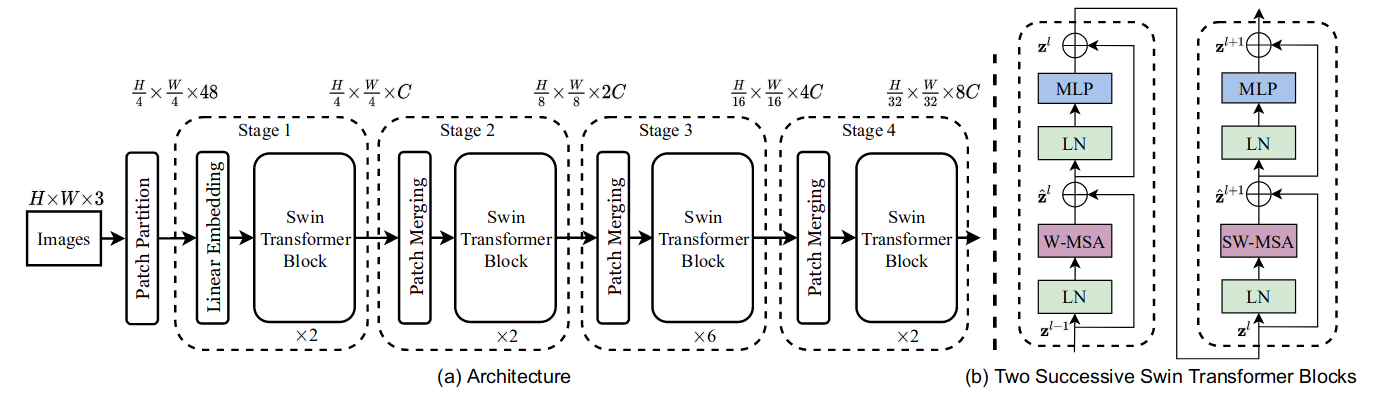
\includegraphics[width=\textwidth]{images/swin_architecture}}
	\caption{
	\textRL{بنية محول}
	\textLR{Swin-Tiny}
	\textLR{\cite{swintransformer}}}
	\label{fig:swin}
\end{figure}
\newline
يبين الشكل 
\ref{fig:swin}
 بنية المحول
\textLR{Swin-Tiny}،
وكما نلاحظ فإن الجزء الأول من المخطط هو
\textLR{patch partition}،
إذ يتم تقسيم الصورة إلى أجزاء 
\textLR{patches}
كما في خوارزمية
\textLR{ViT\cite{ViT}}،
%وهو كما يوضح الشكل
%\ref{fig:swin_patch_partition}،
%يتم بداية تقسيم الصورة إلى نوافذ وهي الخطوط الحمراء في الشكل، وكل نافذة تقسم إلى أجزاء
%\textLR{patches}
%وهي الخطوط الرمادية  كما في خوارزمية
%\textLR{\cite{ViT}}،
%\begin{figure}[!h]
%	\centerline{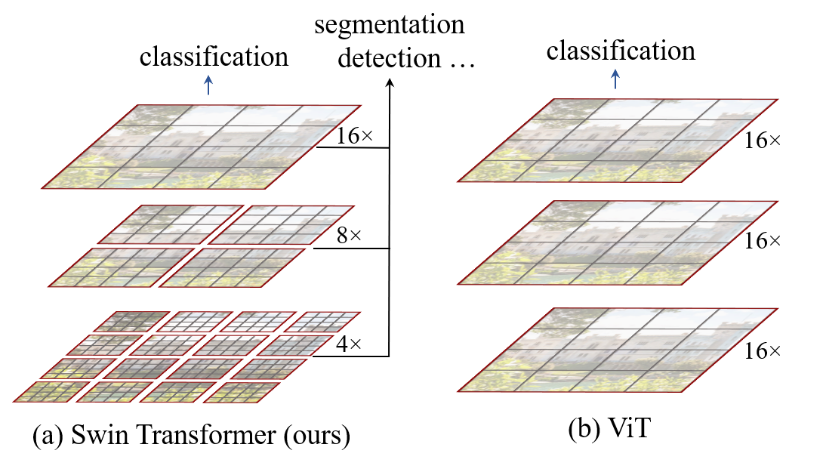
\includegraphics[width=\textwidth]{images/swin_patch_patition.png}}
%	\caption{
%	\textRL{الفرق بين تقسيم النوافذ بين محولي}
%	\textLR{ViT\cite{ViT},Swin\cite{swintransformer}}}
%	\label{fig:swin_patch_partition}
%\end{figure}
حيث يعامل كل جزء معاملة
\textLR{token}،
حجم كل جزء
$4\mathsf{x}4\mathsf{x}3 = 48$،
وبالتالي عدد عناصر سلسلة الدخل أو عدد الـ
\textLR{tokens}
هو
$(\frac{H}{4} \mathsf{x} \frac{W}{4})$.
فيكون دخل المرحلة الأولى
\textLR{stage1}
هو سلسلة بأبعاد
$\frac{HW}{16} \mathsf{x}48$.
\newline
الكتلة الأولى في المرحلة الأولى هي 
\textLR{linear embedding}،
وهي عبارة عن طبقة خطية هدفها إسقاط شعاع السمات السابق إلى بعد 
$C$
أي يصبح
$\frac{HW}{16}\mathsf{x}C$.
ومن ثم يتم تطبيق كتلتي محول 
\textLR{Swin}
متعاقبتين،  بنية الكتلة موضحة في الجزء اليمين من الشكل
\ref{fig:swin}
وسنشرحها في الفقرة القادمة، أبعاد دخل وخرج كتلة محول 
\textLR{Swin}
تبقى ثابتة، أي يكون بعد خرج المرحلة الأولى هو
$\frac{HW}{16}\mathsf{x}C$.
\subsubsection{الهرمية
\textLR{hierarchical}}
نلاحظ بأن الجزء الأول من كل مرحلة تالية هو طبقة
\textLR{patch merging}،
وهو القسم المسؤول عن هرمية النموذج، إذ أن هدف هذه الطبقة الخطية هو تخفيض عدد عناصر سلسلة الدخل أو الـ
\textLR{tokens}،
ويزداد هذا التخفيض  بازدياد عمق النموذج
 كما نلاحظ من أبعاد دخل كل كتلة في الشكل 
\ref{fig:swin}.
\newline
تقوم هذه الطبقة بدمج كل مجموعة
$2\mathsf{x}2$ 
من العناصر المتجاورة وتقوم بسلسلتها فتصبح شعاع واحد بـ$4$ عناصر، وبالتالي يتغير عدد عناصر السلسلة 
فإذا كانت أبعاد السلسلة
$\frac{H}{4}\mathsf{x}\frac{W}{4}\mathsf{x}C$ 
فيصبح
$\frac{H}{8}\mathsf{x}\frac{W}{8}\mathsf{x}4C$،
ومن ثم عبر طبقة خطية تقوم بتغيير أبعاد كل عنصر من السلسلة أو كل 
\textLR{token}
إلى النصف فيصبح
$\frac{H}{8}\mathsf{x}\frac{W}{8}\mathsf{x}2C$،
وهو خرج المرحلة الثانية.
\newline
$\frac{H}{16}\mathsf{x}\frac{W}{16}\mathsf{x}4C$ 
خرج المرحلة الثالثة.
\newline
$\frac{H}{32}\mathsf{x}\frac{W}{32}\mathsf{x}8C$
وهو خرج المرحلة الرابعة والأخيرة في نموذج
\textLR{tiny}.
\newline
إن أبعاد كل مرحلة مشابهة لأبعاد السمات في شبكات
\textLR{CNN}
النموذجية كما في
\textLR{VGG\cite{VGG}, ResNet\cite{ResNet}}
وهذا ما يمكننا من استخدام هذا النموذج كـ
\textLR{backbone}
بديل
لتطبيقات الرؤية الحاسوبية المختلفة.
\subsubsection{كتلة محول
\textLR{Swin}}
نلاحظ من الجزء اليسار من المخطط أن بنية 
\textLR{Swin}
مشابهة لبنية المحول الأصلي، فيما عدا استبدال الانتباه المتعدد الرؤوس 
\textLR{MHA}
بـ انتباه متعدد الرؤوس مع نوافذ
\textLR{W-MHA}
في الكتلة الأولى، وانتباه متعدد الرؤوس مع نوافذ مزاحة 
\textLR{SW-MHA}
في الكتلة التالية.
\subsubsection{التعقيد الحسابي عند استخدام النوافذ}
يوضح الشكل
\ref{fig:swin_shifted_window}
تقسيم النوافذ،
إذ يتم حساب الانتباه الذاتي بين عناصر النافذة الواحدة فقط، وهذا ما يخفض التعقيد الحسابي.
مقارنة بالمحول الأصلي الذي يحسب الانتباه الذاتي بين كل العناصر فإن التعقيد الحسابي من أجل سلسلة دخل بأبعاد 
$hw\mathsf{x}C$ 
يكون: 
\begin{equation}
\Omega(MHA) = 4hwC^2+2(hw)^2C
\end{equation}
نلاحظ أن التعقيد يزداد بشكل تربيعي مع زيادة أبعاد الصورة
بينما في حال استخدام طريقة النوافذ وحساب الانتباه داخل العناصر ضمن النافذة الواحدة فقط فيكون التعقيد الحسابي من أجل كل نافذة تحوي 
$M\mathsf{x}M$ 
جزء أو 
\textLR{patch}
يكون
\begin{equation}
\Omega(W-MHA)=4hwC^2+2M^2hwC
\end{equation}
نلاحظ بأن التعقيد الحسابي متناسب بشكل خطي مع أبعاد الصورة في حال كانت
$M$ 
ثابتة ( في النموذج 
$M=7$
)،
هذا التخفيض في التعقيد الحسابي يجعل من محول 
\textLR{Swin}
مناسب أكثر لتطبيقات الصورة ذات الحجوم الكبيرة و لتطبيقات الزمن الحقيقي.
\subsubsection{النوافذ المزاحة}
\begin{figure}[!h]
	\centerline{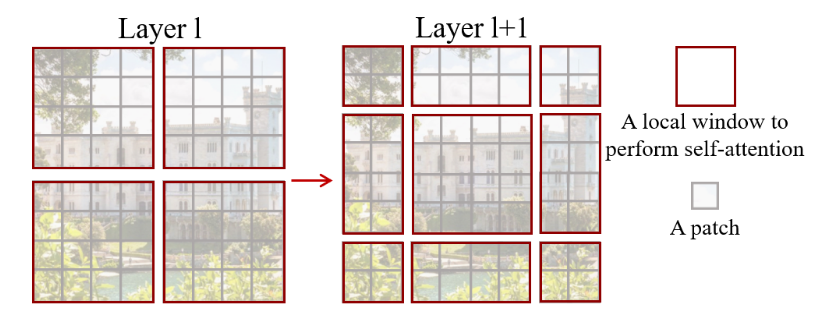
\includegraphics[width=\textwidth]{images/swin_shifted_window.png}}
	\caption{
	\textRL{طريقة النوافذ المزاحة بين كل كتلتين متعاقبتين في محول}
	\textLR{Swin}
	\textLR{\cite{swintransformer}}}
	\label{fig:swin_shifted_window}
\end{figure}
يبين الشكل
\ref{fig:swin_shifted_window}
كيفية اختيار تقسيم النوافذ من أجل كتلتين أو طبقتين متتاليتين من محول 
\textLR{Swin}.
الطبقة الأولى 
$l$
( الصورة اليسار) تقسم النوافذ بشكل نظامي، ويحسب الانتباه الذاتي ضمن أقسام النافذة الواحدة، كل نافذة على حدة.
الطبقة التالية من محول 
\textLR{Swin}
تقسم النوافذ بشكل مزاح عن نوافذ الطبقة السابقة، وذلك بمقدار نصف نافذة إلى جهة اليمين ونصف نافذة إلى الأسفل.
توضح المعادلات 
\ref{eq:swin_SW}
 خرج السمات من أجل كتلتين متعاقبتين لمحول 
\textLR{Swin} 
في مرحلة واحدة.
المعادلة الأولى تحسب الانتباه من أجل تقسيم النوافذ النظامي، الشكل
\ref{fig:swin_shifted_window}
 اليسار.
أما المعادلة الثالثة فهي حساب الانتباه ضمن النوافذ المزاحة، الشكل
\ref{fig:swin_shifted_window}
اليمين
\begin{equation}
	\begin{split}
	&\hat{z}^l = W-MSA(LN(z^{l-1}))+z^{l-1}\\
	&z^l = MLP(LN(\hat{z}^l))+\hat{z}^l\\
	&\hat{z}^{l+1} = SW-MSA(LN(z^l))+z^l\\
	&z^{l+1} = MLP(LN(\hat{z}^{l+1}))+\hat{z}^{l+1}\\
	\end{split}
	\label{eq:swin_SW}
\end{equation}
حيث 
$z_{l-1}$
خرج كتلة محول 
\textLR{Swin}
للمرحلة السابقة.
\subsubsection{تأثير النوافذ المزاحة وفائدتها}
نلاحظ أن النوافذ المزاحة في الطبقة 
$l+1$
تتقاطع مع نوافذ الطبقة 
$l$
ذات التقسيم النظامي، وهذا التقاطع يؤمن اتصال وتبادل معلومات بين النوافذ المجاورة كون الانتباه يحسب ضمن النافذة فقط، ويتجاهل النوافذ الأخرى.
طريقة النوافذ المزاحة قد حسنت من قدرة النمذجة للنموذج وهذا مايوضحه البحث 
\textLR{\cite{swintransformer}}
\subsubsection{الإزاحة الحلقية
\textLR{cyclic-shifting}}
ينتج عن طريقة النوافذ المزاحة زيادة في عدد النوافذ، بحيث لو كان عدد النوافذ في التقسيم النظامي
$\frac{h}{M} \mathsf{x} \frac{w}{M}$
يصبح في طبقة النوافذ المزاحة
$(\frac{h}{M} +1) \mathsf{x} (\frac{w}{M}+1)$،
حيث
$M \mathsf{x} M$
عدد أجزاء النافذة الواحدة. وكما في الشكل 
\ref{fig:swin_shifted_cycled_window}
 فإن بعض النوافذ سيكون حجمها أقل من 
$M\mathsf{x}M$.
أبسط طريقة لحل هذه المشكلة هي بحشو 
\textLR{pad}
النوافذ صغير الحجم لتصبح ببعد 
$M\mathsf{x}M$،
ومن ثم حساب الانتباه الذاتي داخل هذه النافذ  مع حجب القيم المحشوة.
هذا الحل لا يزيد من التعقيد الحسابي للنموذج حين يكون عدد النوافذ صغير، ولكن في حال العدد الكبير للنوافذ فقد اقترح النموذج طريقة الإزاحة الحلقية. 
\begin{figure}[!h]
	\centerline{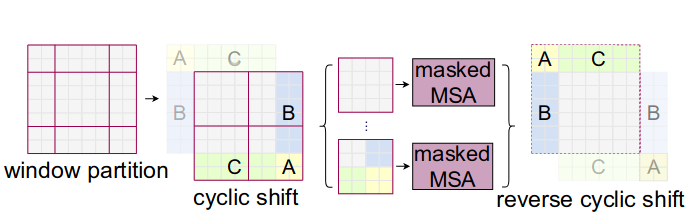
\includegraphics[width=\textwidth]{images/swin_shifted_cycled_window.png}}
	\caption{
		الازاحة الحلقية المستخدمة في محول
		\textLR{Swin}
		\textLR{\cite{swintransformer}}}
	\label{fig:swin_shifted_cycled_window}
\end{figure}
هذه الطريقة كما يوضح الشكل 
\ref{fig:swin_shifted_cycled_window}
 فإنه يتم إعادة ترتيب الأقسام بشكل حلقي حتى يكون عدد النوافذ متساوِ قبل وبعد الإزاحة. وأثناء إعادة الترتيب بشكل حلقي يمكن أن تحتوي النافذة على أجزاء من النوافذ الأخرى غير المجاورة لها،  ولحساب الانتباه الذاتي في هذه الحالة نستخدم تقنية الحجب 
\textLR{masking}
 وذلك لكي لا تدخل النوافذ غير المجاورة في حساب الانتباه الذاتي.
في هذه الحالة نحافظ على عدد النوافذ في حال التقسيم النظامي وفي حال التقسيم المزاح.
بينت التجربة في المقالة
\textLR{\cite{swintransformer}}
أن طريقة الازاحة الحلقية أسرع من طريق الحشو.
\begin{figure}[!h]
	\centerline{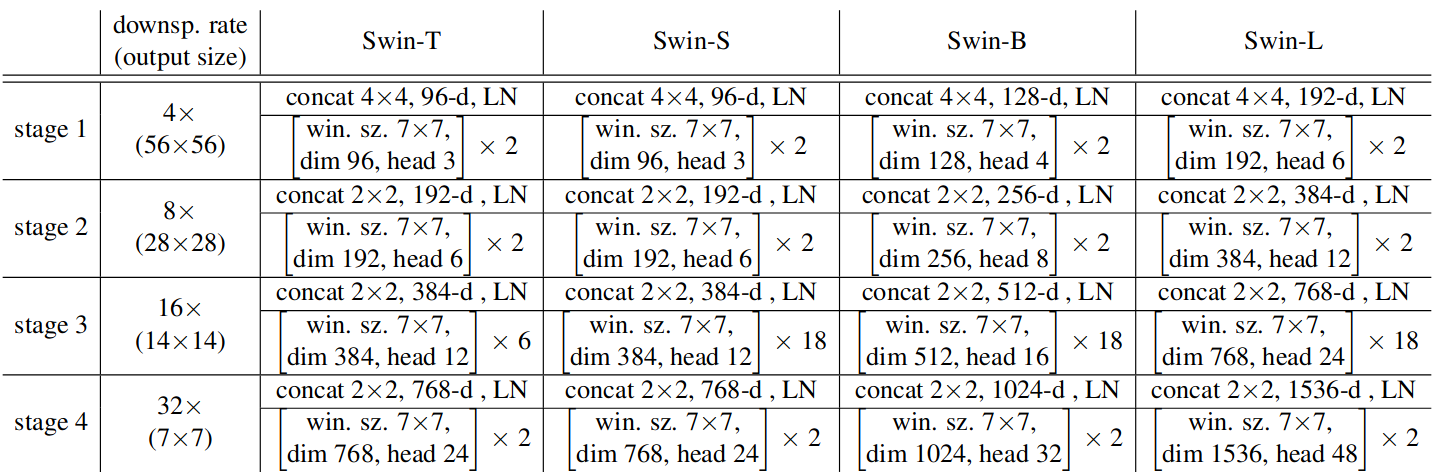
\includegraphics[width=\textwidth]{images/swin_architecture_table.png}}
	\caption{
	\textRL{أبعاد نموذج }
	\textLR{Swin}
	\textRL{من أجل عدة نسخ}
	\textLR{\cite{swintransformer}}}
	\label{fig:swin_architecture_table}
\end{figure}
يبين الجدول 
\ref{fig:swin_architecture_table}
أبعاد كل مرحلة من مراحل محول 
\textLR{Swin}
وذلك من أجل أبعاد مختلفة لصورة الدخل (السطر الأول من الجدول)، من أجل ملاحق
\textLR{Swin} 
فقد تم تدريبه من أجل عدة نسخ من المحول، اخترنا تطوير النسخة التي تستخدم
\textLR{Swin-Tiny}
كونه النموذج الأسرع والأقل كلفة في التدريب.
\section{خلاصة}
نستنتج من خلال الدراسة المرجعية بأن الاتجاه في تطوير نظم الملاحقة السائد يعتمد على التعلم العميق وخاصة نماذج المحول
ومن نتائج الشكل 
\ref{fig:comapre}
نلاحظ بأن خوارزميات الملاحقة ماتزال بحاجة إلى مزيد من البحث والتحسين من ناحية السرعة والأداء.
\section{خاتمة}
عرضنا في هذا الفصل مقدمة عن الملاحقة وأنواعها والمشكلات التي تواجها، وكان التركيز على أنواع ملاحقات التعلم العميق، إذ أن البحث يستهدف ملاحق 
\textLR{SwinTrack-Tiny\cite{swinTrack}}
الذي يعتمد على محول
\textLR{Swin\cite{swintransformer}}
لاستخلاص السمات، إذ أن تصميم هذه النسخة من المحول مناسب لتطبيقات الرؤية الصنعية كالملاحقة بسبب سرعة أداءه.
\\
تحدثناعن نموذج المحول وكيفية تطوره باستخدامه لتوابع الانتباه فقط وبذلك تجنب مشاكل الشبكات العودية، وقد تم شرح بنية المحول الأصلي مع التركيز على شرح تابع الانتباه، والذي استخدمناه لدمج سمات الصور في نموذجنا كما سنتحدث في الفصل القادم. وذكرنا تطبيقات المحول في الرؤية الحاسوبية، مع شرح مفصل لنموذج
\textLR{SwinTransformer}
وبينّا سبب استخدامنا له كونه مناسب لتطبيقات الرؤية الصنعية، إذ أنه أقل تعقيداً من نموذج المحول الأصلي في حال صورة دخل بأبعاد كبيرة.
وفي الفقرة الأخيرة تحدثنا عن تطبيقات المحول في  الملاحقة والتي بدأت منذ $2021$ .











%\chapter{النموذج المقترح}

سنتكلم في هذا الفصل عن خوارزميات الملاحقة التي اعتمدنا عليها بشكل أساسي في بحثنا وهي خوارزمية 
\textLR{SwinTrack \cite{swinTrack}}
\ref{section:swintrack}
التي تعتمد على محول 
\textLR{Swin \cite{swintransformer}}
كـ
\textLR{backbone}،
وتستخدم بنية مرمز - مفكك ترميز
%\textLR{encoder-decoder}
بتوابع انتباه متعدد الرؤوس 
\textLR{MHA}.
مشكلة هذه الخوارزمية أنها تستخدم المعلومات المكانية (معلومات المظهر) فقط لتقدير حالة الغرض، بينما تتجاهل بشكل تام المعلومات الزمانية.
\newline
استفدنا من خوارزمية 
\textLR{STARK \cite{Stark}} \ref{section:stark}
لإدخال المعلومات الزمانية، وذلك عن طريق تحديث الـ
\textLR{template}
وإدخاله كدخل ثالث إلى النموذج مع الاحتفاظ بالـ 
\textLR{template}
الابتدائي.
وسنشرح أيضاً كيفية الاستفادة من الـ
\textLR{template}
المحدّث دون تغيير أبعاد النموذج للاستفادة من النموذج الأصلي المدرب مسبقاً، وهو التعديل الأساسي في بحثنا.
\newline
سنبدأ بشرح عام عن خوارزمية 
\textLR{STARK}
كوننا سنحاكي طريقة الخوارزمية في تحديث صورة الهدف.
\section{\textLR{STARK\cite{Stark}} \label{section:stark}}
\textRL{وهي اختصار لـ
\textLR{\textbf{s}patio-\textbf{t}emporal tr\textbf{a}nsfo\textbf{r}mer network for visual trac\textbf{k}ing}}،
في المقالة 
\textLR{\cite{Stark}}
 هناك نموذجان، النموذج الأول يستخدم فقط المعلومات المكانية لتحديد مكان الهدف، والنموذج الثاني هو بإضافة المعلومات الزمانية إلى النموذج الأول وذلك باستخدام 
\textLR{template}
\textRL{محدّث}
كدخل ثالث إلى النموذج. وهذه الطريقة لإدخال المعلومات الزمانية هي التي استخدمناها لتعديل خوارزمية 
\textLR{SwinTrack\cite{swinTrack}}.
\subsection{نموذج
\textLR{STARK}
الأول (مع المعلومات المكانية فقط)
}
البنية الأولية من خوارزمية 
 \textLR{STARK}
 والتي تستخدم فقط المعلومات المكانية موضحة في الشكل
 \ref{stark_base}،
\begin{figure}[!h]
	\centerline{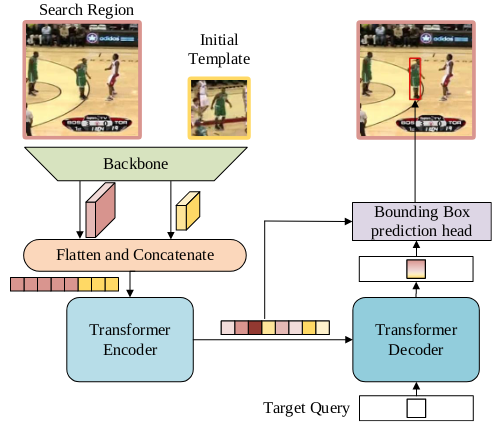
\includegraphics[scale=0.5]{images/stark_base}}
	\caption{
		\begin{footnotesize}
		\textRL{مخطط النموذج الأول من خوارزمية}
		\textLR{STARK}
		\textRL{والذي يستخدم المعلومات المكانية فقط}
		\textLR{\cite{Stark}}
		\end{footnotesize}
	}
	\label{stark_base}	
\end{figure}
للنموذج دخلان هما الـ
\textLR{template}
 من الإطار الأول لعملية الملاحقة 
$Z \in \Re^{{3} \mathsf{x} {H_z} \mathsf{x} W_z}$
حيث 
$H_z = W_z = 128$،
ونافذة البحث 
$X \in \Re^{{3} \mathsf{x} {H_x} \mathsf{x} W_x}$
حيث
$H_x = W_x = 320$.
\subsubsection{المرحلة الأولى - استخلاص السمات}
يتم استخلاص سمات كل من الدخلين عبر 
\textLR{backbone}،
 وهي المراحل الأربعة الأولى من شبكة
\textLR{ResNet\cite{ResNet}}،
فيكون
\textLR{stride}
 الشبكة 
 $s = 16$.
\newline
 خرج الـ
\textLR{backbone}
 هو سمات كل من الـ
\textLR{template}
$f_z \in \Re^{C \mathsf{x} \frac{H_z}{s} \mathsf{x} \frac{W_z}{s}}$،
وسمات نافذة البحث
$f_x \in \Re^{C \mathsf{x} \frac{H_x}{s} \mathsf{x} \frac{W_x}{s}}$.
بعدها  يتم سَلسَلة
\textLR{concatenate}
 سمات الـ
\textLR{template}
وسمات نافذة البحث ضمن سلسلة واحدة، ومن ثم تخفيض أبعاد السلسلة من 
\textLR{C}
إلى
\textLR{d}
، ثم تسطيح 
\textLR{flatten} 
 السلسلة لتصبح بأبعاد
$( d \mathsf{x} \frac{H_z}{s}\frac{W_z}{s} + \frac{H_x}{s}\frac{W_x}{s} )$،
وهذه السلسلة هي دخل المحول.
\subsubsection{المرحلة الثانية - المحول}
%تعتمد بنية المحول في هذه الخوارزمية بشكل كبير على محول  خوارزمية الكشف 
%\textLR{DETR\cite{DETR}}
%مع اختلافات طفيفة مثل عدد
%\textLR{target queries}.
يحتوي المرمز على $6$ طبقات، عدد الرؤوس في تابع الانتباه الذاتي متعدد الرؤوس
$ h=8 $,
أما أبعاد الطبقة المخفية  في شبكات 
\textLR{MLP}
فهي
 $2048$،
الترميز المكاني هو 
\textLR{sinusoidal}
كما في المحول الأصلي.
\newline
هدف  المرمز هو تعديل السمات بحسب السياق وإرسالها إلى مفكك الترميز.
من الشكل
\ref{stark_base}
نلاحظ دخلين لمفكك الترميز
الأول هو خرج المرمز، أما الثاني فهو
\textLR{target query}.
إن بنية المحول في
\textLR{STARK}
تعتمد بشكل كبير على المحول المستخدم في كاشف
\textLR{DETR\cite{DETR}}،
حيث عدد
\textLR{target queries}
هي عدد الأغراض التي يجب الكشف عنها. هنا في 
\textLR{STARK}
كخوارزمية ملاحقة لغرض واحد فإن عدد 
\textLR{target queries = 1}.
 \subsubsection{المرحلة الثالثة - تقدير مكان الهدف }
لتقدير المستطيل المحيط  بالغرض اعتمدت 
\textLR{STARK}
على الكتلة الموضحة في الشكل 
\ref{stark_score_head}
\begin{figure}[!h]
	\centerline{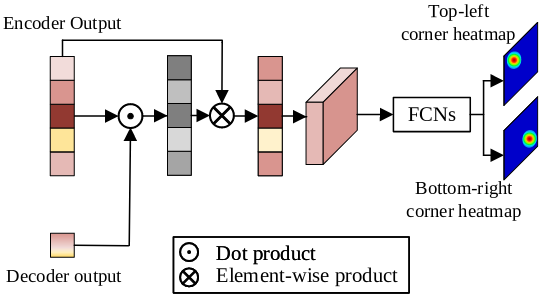
\includegraphics[scale=0.5]{images/stark_score_head}}
	\caption{
		\textRL{شبكة الـ}
		\textLR{regression}
		\textRL{لتقدير مكان الغرض}
		\textLR{\cite{Stark}}}
	\label{stark_score_head}
\end{figure}
هدف هذه الشبكة هو الـ
\textLR{regression}
، أي تقدير إحداثيات  الزاوية العليا اليسارية و الزاوية السفلى اليمينية للمستطيل المحيط.
بداية يحسب التشابه بين خرج المرمز وخرج مفكك الترميز،
 وذلك بحساب الجداء السلمي بينهما. نعدل خرج المرمز بتوزينه بقيم التشابه المحسوب سابقاً، نعدل من شكل خريطة السمات لتصبح ب
 $3$
  أبعاد 
$f \in \Re^{d \mathsf{x} \frac{H_s}{s} \mathsf{x} \frac{W_s}{s}}$.
ونقوم بإدخال خريطة السمات إلى شبكة 
\textLR{FCN}
 مكونة من $ 5$ طبقات تلاففية
\textLR{Conv-BN-ReLU}
 مع تابع تفعيل 
\textLR{ReLU}.
والخرج عبارة عن خريطة احتمالية لزوايا المستطيل المحيط.
\subsubsection{تابع الخطأ}
تابع الخطأ المستخدم في التدريب هو مجموع موزن لتابعين، الأول هو تابع الخطأ 
$L_1$،
والثاني هو
\textLR{GIOU\cite{giou}}
بحسب المعادلة التالية :
\begin{equation}
L = \lambda_{giou} L_{giou}(b_i,\hat{b}_i) + \lambda_{L_1} L_1(b_i,\hat{b}_i)
\label{loss_regression}
\end{equation} 
حيث 
$b_i$
هي القيمة الحقيقية 
\textLR{ground truth}
للمستطيل المحيط، بينما
$\hat{b}_i$
هي القيمة المقدرة (خرج الملاحق)، 
$\lambda_{giou},\lambda_l$
هي
\textLR{hyperparameters}.
\subsection{نموذج 
\textLR{STARK}
الثاني - مع المعلومات المكانية والزمانية}
معظم الملاحقات الحديثة تعتمد فقط على المعلومات المكانية أي معلومات مظهر الهدف وتتجاهل المعلومات الزمنية
\textLR{\cite{swinTrack},\cite{SiamFC}}.
حاولت خوارزمية
\textLR{STARK} 
إدخال المعلومات الزمانية عن طريق دخل ثالث وهو صورة الهدف في آخر عملية ملاحقة، وندعوه بالـ 
\textLR{dynamic template}.
هذا الـ
\textLR{template}
 الجديد الذي يحوي معلومات تغير مظهر الهدف هو ما نعتبره يحمل المعلومات الزمانية، بالإضافة إلى احتفاظ النموذج بالـ
\textLR{template}
الابتدائي.
\newline
يوضح الشكل 
\ref{stark-full}
النسخة الثانية 
(اللون الأحمر) على النسخة الأولية (اللون الأزرق) لخوارزمية 
\textLR{STARK}.
\begin{figure}[!h]
	\centerline{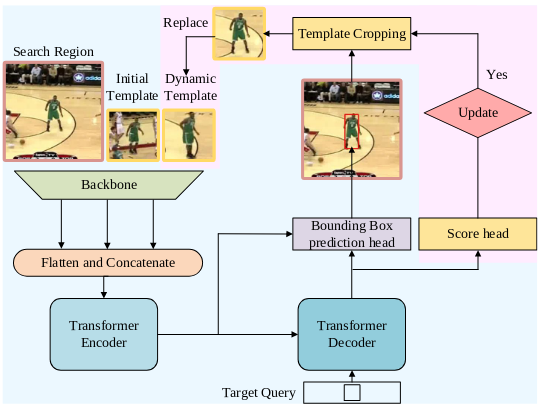
\includegraphics[width=\textwidth]{images/stark_full}}
	\caption{
		\textRL{النسخة الثانية من محول}
		\textLR{STARK}
		\textRL{باستخدام المعلومات الزمانية والمكانية}
		\textLR{\cite{Stark}}}
\label{stark-full}
\end{figure}
وكما في النموذج الأول يتم استخلاص سمات الـ
\textLR{template}
الجديد عبر
\textLR{backbone}،
و تكون مهمة المرمز هي استخلاص السمات المكانية والزمانية من شعاع سمات
 المداخل الثلاثة بعد سَلسَلتها.
\newline
التعديل الثاني في الخوارزمية هو معيار تحديث الهدف،
تم استخدام شبكة
\textLR{score head}
 غرضها التصنيف (هدف أو خلفية)،
% خرجها ندعوه بـ
%\textLR{score}،
يعبر خرجها
(\textLR{score})
 عن احتمالية وجود هدف في الموقع المقابل.
تحتوي الشبكة على ثلاث طبقات
\textLR{MLP}
%نسميها 
%\textLR{score head}،
بُعد الطبقة المخفية $256$، مع تابع تفعيل 
\textLR{sigmoid}.
\newline	
يتم تدريبها بتابع
\textLR{BCE binary cross-entropy}،
بحيث يكون خرج الشبكة
%(\textLR{score})
قيمة عالية عندما تكون وثوقية الهدف أكبر، 
\textRL{ولا يتم التحديث إلا }
عندما تكون هذه القيمة أكبر من حد معين
\textLR{threshold}،
تكون الوثوقية عالية طالما أن نافذة البحث تحوي كامل الهدف.
\newline
لتسهيل عملية تدريب النموذج الكلي
يتم تدريب النموذج على مرحلتين،
المرحلة الأولى يتم تدريب الشبكة بالكامل ماعدا شبكة التصنيف،
%\textLR{score head}،
أي باستخدام تابع الخطأ في المعادلة
\ref{loss_regression}.
المرحلة الثانية هي بتجميد أوزان المرحلة السابقة، وتدريب شبكة التصنيف
%\textLR{score head}
فقط، وذلك باستخدام تابع خطأ
\textLR{BCE}
كما في المعادلة
\ref{BCE}
\begin{equation}
	L_{ce} = log(P_i) + (1-y_i)log(1-P_i)
	\label{BCE}
\end{equation}
حيث
$y_i$
هي القيمة الحقيقة
\textLR{ground truth}،
$Pi$
هي خرج شبكة التصنيف.
\newline
أثناء التدريب يتم اختيار الـ
\textLR{template}
\textRL{الابتدائي}،
الـ
\textLR{template}
الديناميكي
\textRL{ ونافذة البحث}
بشكل عشوائي من
\textRL{القيم الحقيقية}
لمعطيات التدريب
\textRL{لنفس الفيديو}،
بحيث لا يكون البعد بينهما (عدد الإطارات) أكبر من قيمة ندعوها بـ
\textLR{update interval}.
طريقة التدريب هذه استعنّا بها عند تدريب النموذج الخاص بالبحث.
\newline
في مرحلة الملاحقة يتم تحديث الـ
\textLR{template}
 الديناميكي فقط عندما يكون عدد الإطارات بعد آخر تحديث أكبر من  
\textLR{update interval = 200}،
ويكون
$score > 0.5$.
\newline
يبين الجدول 
\ref{table:two_tracker_got10k_results}
نتائج التدريب على مجموعة المعطيات
\textLR{got10k}،
حيث
\textLR{STARK-S50}
 هي النسخة الأولى من الخوارزمية باستخدام المعلومات المكانية فقط، أي دون الـ
\textLR{template}
 الديناميكي، وباستخدام 
\textLR{ResNet50}
 كـ
\textLR{Backbone}.
\newline
\textLR{STARK-ST101}
 هي النسخة الثانية من الخوارزمية، أي باستخدام المعلومات المكانية والزمانية، وباستخدام
\textLR{ResNet101}
 كـ
\textLR{backbone}.
\newline
%****
البنية الصلبة المستخدمة في تدريب واختبار كلا النموذجين هي
\textLR{8 X 16GB Tesla V100 GPU}.
\newline
\textRL{
من الجدول 
\ref{table:two_tracker_got10k_results}
نلاحظ تحسن أداء خوارزمية 
\textLR{STARK}
عند إضافة الـ
\textLR{template}
المحدّث دون 
}
\textRL{
التأثير على سرعة الأداء، مع زيادة طفيفة في حجم النموذج في حال استخدام نفس الـ 
\textLR{backbone}.
}
% \selectlanguage{english}
%\begin{figure}[H]
%	\centering
%	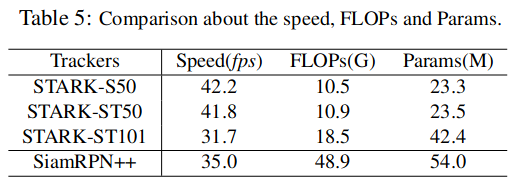
\includegraphics[width=\textwidth]{images/stark_speed}
%	\caption{
%		\cite{Stark}
%		speed of stark
%	}
%\end{figure}
%\selectlanguage{arabic}
\section{\textLR{SwinTrack\cite{swinTrack}}\label{section:swintrack}}
الفكرة الأساسية من البحث هي تعديل ملاحق
\textLR{SwinTrack}
بإدخال المعلومات الزمانية، وذلك بالاستفادة من التعديل المستخدم في ملاحق 
\textLR{STARK}
\ref{section:stark}. 
لذلك سنشرح في هذه الفقرة خوارزمية 
\textLR{SwinTrack}
بشيء من التفصيل، كونها النموذج الأساسي في بحثنا.
\newline
هذا الملاحق يعتمد كلياً على توابع الانتباه لاستخلاص ودمج السمات، إذ أنه يستخدم محول
\textLR{Swin\cite{swintransformer}}
كـ
\textLR{backbone}
لاستخلاص السمات، وبذلك فهو يختلف عن الملاحقات السابقة التي تستخدم المحول كجزء من بنيتها، وتستفيد من شبكات
\textLR{CNN}
%كشبكة
%\textLR{ResNet\cite{ResNet}}
%وشبكة
%\textLR{AlexNet\cite{alexnet}}
لاستخلاص سمات الصور، وذلك كما في خوارزميات الملاحقة
\textLR{Transformer Tracking\cite{transformertracker}}
و
\textLR{STARK\cite{Stark}}.
أما بالنسبة لخوارزمية الملاحقة 
\textLR{SwinTrack}
فهي تستخدم بنية  مرمز- مفكك ترميز
%\textLR{encoder-decoder}
لدمج السمات والتي تعتمد على توابع الانتباه كما في المحول الأصلي
\textLR{\cite{Vaswani17}}. 

\begin{figure}[!h]
	\centerline{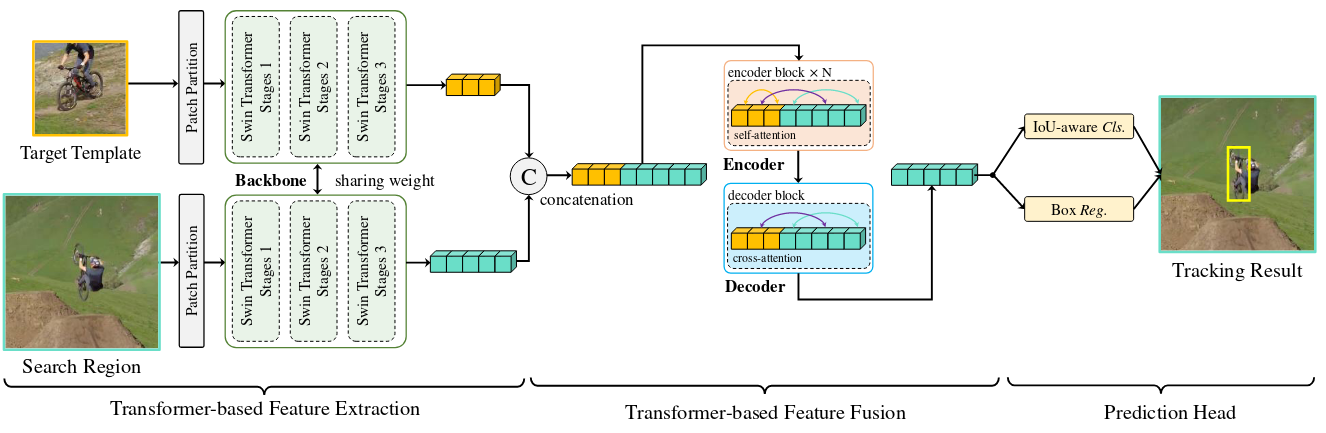
\includegraphics[width=\textwidth]{images/swinTrack}}
	\caption{
		\textRL{بنية الملاحق}
		\textLR{SwinTrack}
		\textLR{\cite{swinTrack}}}
	\label{fig:swintrack}	
\end{figure}
يوضح الشكل 
\ref{fig:swintrack}
مراحل خوارزمية 
\textLR{SwinTrack}،
وهي بشكل أساسي تتكون من ثلاث مراحل، الأولى لاستخلاص السمات، والثانية لدمجها، والثالثة لتحديد مكان وأبعاد الغرض، وسنشرح في الجزء التالي كل مرحلة من هذه المراحل.
\subsection{المرحلة الأولى - استخلاص السمات}
تستخدم هذه الخوارزمية  المراحل الثالث الأولى من محول
\textLR{Swin}
كـ
\textLR{backbone}.
وبمقارنة محول
\textLR{Swin}
بشبكات
\textLR{CNN}
الأخرى
\textLR{\cite{alexnet}\cite{ResNet}}،
 فإن محول
\textLR{Swin}
قادر على إعطاء تمثيل للسمات بشكل أفضل
\textLR{\cite{swintransformer}}.
يوضح الشكل 
\ref{fig:swintrack}
مداخل نموذج الملاحقة 
\textLR{SwinTrack}،
حيث له دخلان الأول هو صورة الـ 
\textLR{template}
الإبتدائي،
والثاني هو نافذة البحث.
\newline
تم تجريب ثلاث نسخ من محول 
\textLR{Swin}
كـ
\textLR{backbone}.
وفيما يلي أبعاد كل نموذج بحسب الـ
\textLR{backbone}
المستخدمة:

\selectlanguage{english}
	\begin{itemize}
		\item SwinTrack-T
		\newline
		Backbone: Swin Transformer-Tiny\cite{swintransformer}
		\newline
		Template size: [112 x 112]; Search region size [224 x 224]; C = 384; N=4
		
		\item SwinTrack-B
		\newline
		Backbone: Swin Transformer-Base\cite{swintransformer}
		\newline
		Template size: [112 x 112]; Search region size [224 x 224]; C = 512; N=8
		
		\item SwinTrack-B-384
		\newline
		Backbone: Swin Transformer-Base\cite{swintransformer}
		\newline
		Template size: [192 x 192]; Search region size [384 x 384]; C = 512; N=8
	\end{itemize}
\selectlanguage{arabic}
حيث $C$ هو بعد النموذج و
$s=16$
هو 
\textLR{stride}
الشبكة،
\textRL{
		و
		$N$
		عدد كتل المرمز
}.
\newline
\subsection{المرحلة الثانية - دمج السمات بالاعتماد على المحول}
يتم سَلسَلة سمات الـ
\textLR{template}
وسمات نافذة البحث ضمن تمثيل موحد $U$ يشكل دخلاً للمرمز.
وكما في المحول الأصلي فإن المرمز يتكون من 
توابع انتباه ذاتي متعددة الرؤوس 
\textLR{MSA}،
مع شبكة عصبونية 
\textLR{FFN}
تتكون من طبقتين مع تابع تفعيل
\textLR{GELU}
\textLR{Gaussian Error Linear Unit}،
مع وجود تنظيم خطي 
\textLR{Linear Normalization}
قبل كل كتلة
\textLR{\textLR{FFN} + MSA}،
و 
\textLR{Residual connection}
 بعد كل كتلة 
\textLR{\textLR{FFN} + MSA}،
وذلك بحسب المعادلات 
\ref{eq:swinencoder}
\begin{equation} \label{eq:swinencoder}
\begin{split}
 &U^1 = Concat(z^1,x^1)\\
 &...\\
 &U^{l^\prime} = U^l + MSA(LN(U^\prime))\\
 &U^{l+1} = U^{l^\prime} + FFN(LN(U^{l^\prime}))\\
 &...\\
 &z^L,x^L = Deconcat(U^L)
\end{split}
\end{equation}


حيث $l$ هي رقم الطبقة، $L$ عدد طبقات المرمز.
كما نرى في آخر معادلة وبحسب الشكل
\ref{fig:swintrack}
فإنه يتم إعادة فصل 
\textLR{deconcatenate}
خرج المرمز وتقسيمه إلى سمات الـ
\textLR{template}
وسمات نافذة البحث.
\newline
يتبع نموذج المحول الأصلي
\textLR{\cite{Vaswani17}}
الطريقة التقليدية في
دمج ومعالجة السمات الآتية من مصادر مختلفة (المصدران في حالتنا هما
\textLR{template}،
ونافذة البحث)، وذلك بحساب الانتباه الذاتي لكل مصدر أي لصورة ال
\textLR{template}
ولصورة نافذة البحث بشكل مستقل، ومن ثم دمج هذه السمات عن طريق 
\textLR{cross-attention}.
هذه الطريقة تدعى بـ
$"$
دمج السمات بالاعتماد على الانتباه التقاطعي
$"$.
%\textRL{بالاعتماد}
% على
%\textLR{cross-attention}$"$.
\newline
أما الطريقة المتبعة في ملاحق
\textLR{Swin}
هي بدمج السمات في دخل المرمز ومعالجتها كسلسلة واحدة، وتسمى بـ
$"$
دمج السمات بالاعتماد على السَلسَلة
\textLR{concatenation-based fusion}
$"$.
وبمقارنة هذه الطريقة بالطريقة السابقة فإنها تخفض التعقيد الحسابي وذلك بانقاص عدد أوزان النموذج، 
\textRL{وبالتالي فهي مناسبة أكثر لتطبيقات الزمن الحقيقي}
\newline
تابع الانتباه هو التابع المستخدم في المحول الأصلي
\textLR{\cite{Vaswani17}}،
إذ لا حاجة لاستخدام تابع انتباه
\textLR{Swin}،
لأن الفرق في التعقيد الحسابي بين التابعين بسيط في حالة دخل صغير الأبعاد، والدخل هنا هو أشعة السمات.
\newline
ترميز الموقع
\textLR{Positional Encoding PE}:
لمساعدة النموذج على تمييز مصادر وأماكن السمات التي تتم معالجتها لابد من إضافة ترميز مكاني إلى السمات، والنوع المستخدم في 
\textLR{SwinTrack}
هو 
\textLR{Untied Positional Encoding\cite{untiedPE}}.
\newline
أما بالنسبة لدخل  مفكك الترميز
 فهو عبارة عن السمات الخارجة من المرمز، وخرجه هو خريطة السمات المعدلة لنافذة البحث
$ x \in \Re^{\frac{H_x}{s} \mathsf{x} \frac{W_x}{s} \mathsf{x} C}$.
تتبع العمليات الحسابية ضمن مفكك الترميز
المعادلات 
\ref{eq2}:
\begin{equation} \label{eq2}
\begin{split}
&U^D = Concat(z^l,x^l)\\
&x^{L^\prime} = x^L + MCA(LN(x^L),LN(U^D))\\
&x = x^{L^\prime} + FFN(LN(x^{L^\prime})).\\
\end{split}
\end{equation}
يحسب تابع الانتباه التقاطعي متعدد الرؤوس
\textLR{MCA}
بين
$x^L$
 خريطة سمات نافذة البحث بعد فك السلسلة، وبين 
$U^D$
%\textLR{Ud}
خرج المرمز والذي يعبر عن سمات كل من الـ
\textLR{template}
ونافذة البحث.
\subsection{المرحلة الثالثة - شبكتي التصنيف وال 
\textLR{regression}
	: }
الخرج النهائي لمفكك الترميز
هو سمات نافذة البحث
$x \in \Re^{\frac{H_x}{s} \mathsf{x} \frac{W_x}{s} \mathsf{x} C}$،
هذه السمات بحاجة إلى معالجة لتحديد موقع الغرض بالنسبة لنافذة البحث.
\newline
يتم استخدام طريقتي التصنيف والـ  
\textLR{regression}
  بشكل منفصل لتحديد موقع الغرض والمستطيل المحيط به.
كل من الكتلتين عبارة عن شبكة عصبونية
\textLR{MLP}
تتكون من ثلاث طبقات، ودخل كل من الشبكتين هو خرج مفكك الترميز.
\newline
الكتلة الأولى هدفها التصنيف ضمن صنفين هما الهدف والخلفية، وخرجها هو خريطة استجابة التصنيف
\textLR{classification response map}
$r_{cls} \in \Re^{(H_x \mathsf{x} W_x) \mathsf{x} 1}$،
بحيث تكون قيمة كل عنصر من عناصر المصفوفة  ضمن المجال
$[0,1]$،
وهذه القيمة تعبر عن احتمالية وجود الغرض في هذا الموقع.
\newline
أما الكتلة الثانية وهي الـ 
\textLR{regression}،
فغايتها التنبؤ بالمستطيل المحيط، وخرجها 
$r_{reg} \in \Re^{(H_x \mathsf{x} W_x) \mathsf{x} 4}$،
كل عنصر من عناصر الخرج يعبر عن إحداثيات الزاوية العليا اليسارية و الزاوية السفلى اليمينية  للمستطيل المحيط.
\newline
%يتم معالجة خرج الشبكتين لتحديد موقع الغرض، فمثلا تم افتراض أن حركة الهدف انسيابية فيتم استخدام 
%\textLR{Hanning penalty}
%للحد من الحركات الكبيرة.
%وفي النهاية
لتحديد موقع الغرض يتم اختيار المستطيل المقابل لأعلى استجابة تصنيف.
وكما لاحظنا من بنية الملاحق فإنه يعتمد بشكل كلي على مظهر الغرض في الإطار الأول للملاحقة دون الأخذ بعين الاعتبار تغيرات شكل الغرض. 
%\textLR{AdamW\cite{AdamW}}
\begin{table}[!h]
	\centering
	\begin{tabular}{c c c c c c c} 
		\hline
		\textLR{Tracker} & $mAO$\% & $mSR_{50\%}$ & $mSR_{75\%}$ &\textLR{Speed($fps$)}&\textLR{FLOPS(G)}&\textLR{Params(M)}\\ [0.5ex] 
		\hline\hline
		\textLR{STARK-S50} &$67.2$&$76.1$&$61.2$&$41.8$&$10.5$&$32.3$\\
		\textLR{STARK-ST50} & $68.0$ & $77.7$ & $62.3$&$41.8$&$10.9$&$32.5$\\ 
		\textLR{STARK-ST101} &$68.8$ & $78.1$ & $64.1$&$31.7$&$18.5$&$42.4$\\
		\hline
		\textLR{SwinTrack-T} & $69.0$ & $78.1$ & $62.1$&$98$&&$23$ \\
		\textLR{SwinTrack-B} & $69.4$ & $78.0$ & $64.3$&$52$&&$91$ \\
		\textLR{SwinTrack-B} &&&&$45$&&$91$\\[1ex] 
		\hline
	\end{tabular}
	\caption{
		\textRL{نتائج خوارزميتي}
		\textLR{SwinTrack,STARK}
		\textRL{من أجل معطيات التدريب}
		\textLR{GOT-10k\cite{got10k}}}
	\label{table:two_tracker_got10k_results}
\end{table}
\newline
%\begin{table}[!h]
%	\centering
%	\begin{tabular}{c c c c c c c} 
%		\hline
%		\textLR{Tracker} & \textLR{AUC}\% & \textLR{Normalized Precision} & \textLR{Precision}&\textLR{Year}\\ [0.5ex] 
%		\hline\hline
%		\textLR{SwinTrack-B-384} &$70.2$&$78.4$&$75.3$&$2021$\\
%		\textLR{STARK} & $67.1$ & $77.0$ &&$2021$\\ 
%		\textLR{TransT} &$64.9$ & $73.8$ & $69.0$&$2021$\\
%		\textLR{TrTr} & $55.1$ &&&$2021$&\\[1ex] 
%		\hline
%	\end{tabular}
%	\caption{
%		\textRL{نتائج خوارزميتي}
%		\textLR{SwinTrack,STARK}
%		\textRL{من أجل معطيات التدريب}
%		\textLR{GOT-10k\cite{got10k}}}
%	\label{table:many_tracker_got10k_results}
%\end{table}

 يوضج الجدول
 \ref{table:two_tracker_got10k_results}
نتائج اختبار خوارزميتي 
\textLR{STRAK\cite{Stark}}
و
\textLR{SwinTrack\cite{swinTrack}}
من أجل مجموعة المعطيات 
\textLR{GOT-10k\cite{got10k}}.
نلاحظ تفوق خوازمية
\textLR{SwinTrack}
في الأداء والسرعة على خوارزمية
\textLR{STARK}.
ونلاحظ أن النسخة
\textLR{SwinTrack-T}
أسرع بمرتين تقريبا من النسخ الأخرى، وهذا ما شجعنا على استخدامها كنموذج أساسي في بحثنا، وتطوير هذه الخوارزمية للحصول على أداء أفضل مع سرعة ملاحقة عالية.
\iffalse
\begin{table}[H]
	\centering
	\begin{tabular}{||p{2.cm}||p{2.cm}||p{2.cm}||p{2.cm}||}
		\hline
		Tracker 	& SwinTrack-Tiny-t4 &\\
		\hline
		SS   		& 79.7 \\
		PS 			& 71.6 \\ 
		NPS 		& 90.1 \\ 
		AO 			& 81.2 \\ 
		SR$_{50\%}$ & 91.1 \\ 
		SR$_{75\%}$ & 79.0 \\
		FPS 		& 66.6\\
		HW 			& NVIDIA GeForce RTX 3060 Laptop GPU\\
		\hline
	\end{tabular}
	\caption{SS : Success Score ,PS : Precision Score , NPS : Normalized Precision Score.
	\newline
	validation}
	\label{table:1}
\end{table}

\label{table:2}
\fi

%
%%report
%\begin{table}[!h]
%	\centering
%	\begin{tabular}{c c c c c c c} 
%		\hline
%		\textLR{Tracker} & $mAO$\% & $mSR_{50\%}$ & $mSR_{75\%}$ &\textLR{Speed($fps$)}&\textLR{FLOPS(G)}&\textLR{Params(M)}\\ [0.5ex] 
%		\hline\hline
%		\textLR{STARK-S50} &$67.2$&$76.1$&$61.2$&$41.8$&$10.5$&$32.3$\\
%		\textLR{STARK-ST50} & $68.0$ & $77.7$ & $62.3$&$41.8$&$10.9$&$32.5$\\ 
%		\textLR{STARK-ST101} &$68.8$ & $78.1$ & $64.1$&$31.7$&$18.5$&$42.4$\\
%		\hline
%		\textLR{SwinTrack-T} & $69.0$ & $78.1$ & $62.1$&$98$&&$23$ \\
%		\textLR{SwinTrack-B} & $69.4$ & $78.0$ & $64.3$&$52$&&$91$ \\
%		\textLR{SwinTrack-B} &&&&$45$&&$91$\\[1ex] 
%		\hline
%	\end{tabular}
%	\caption{
%		\textRL{نتائج خوارزميتي}
%		\textLR{SwinTrack,STARK}
%		\textRL{من أجل معطيات التدريب}
%		\textLR{GOT-10k\cite{got10k}}}
%	\label{table:two_tracker_got10k_results}
%\end{table}
%	
\section{النموذج المقترح\label{section:my_model}}
كما ذكرنا فإن معظم الملاحقات الحديثة تستخدم المعلومات المكانية فقط أي  معلومات مظهر الهدف. كما في 
\textLR{SwinTrack\cite{swinTrack}}
 وغيرها. 
لكن كان هناك بعض المحاولات للاستفادة من المعلومات الزمانية كما في  خوارزمية
\textLR{STARK\cite{Stark}}،
وذلك من خلال إدخال صورة الغرض الجديد الناتج عن الملاحقة كدخل ثالث، كما هو مذكور في الفقرة 
\ref{section:stark}.
\newline
أما في خوارزمية
\textLR{SwinTrack}
والتي هي النموذج الأساسي في بحثنا، فإنها تعتمد فقط على الـ
\textLR{template}
المأخوذ من أول إطار في الملاحقة كدخل أول، ونافذة البحث كدخل ثاني، أي أن التغيرات التي تطرأ على الغرض لا يتم أخذها بعين الاعتبار.
\newline
الفكرة الأساسية من البحث هي الاستفادة من المعلومات الزمانية، كما في ملاحق 
\textLR{STARK\cite{Stark}}،
لتعديل نموذج
\textLR{SwinTrack\cite{swinTrack}}،
وذلك بأخذ صورة الغرض الناتجة عن الملاحقة
و سنسميها
\textLR{dynamic template}
أو الـ
\textLR{template}
الجديد
كدخل ثالث للخوارزمية.
\newline
وكما هو موضح في المخطط 
\ref{fig:my_model}
والذي يوضح التعديل الذي قمنا به على خوارزمية 
\textLR{SwinTrack\cite{swinTrack}}،
 فإن خوارزميتنا تستخرج سمات الـ
\textLR{template}
الجديد
عبر 
\textLR{Swin backbone}،
فيصبح لدينا سمات الـ
\textLR{template}
الابتدائي و سمات الـ
\textLR{template}
الجديد
بحاجة إلى دمج ومعالجة.
\newline 
كان لدينا عدة خيارات لدمج سمات الـ
\textLR{template}
الجديد:
\begin{itemize}
\item
الخيار الأول كما في ملاحق
\textLR{STARK}
وملاحق
\textLR{SwinTrack}
بأن يتم الدمج عن طريق سَلسَلة
\textLR{concatenate} 
سمات الثلاث مداخل في سلسلة واحدة، ونستخدمها كدخل للمرمز لتدريبه على كشف المعلومات الزمانية والمكانية معاً.
\newline
يتطلب هذا الخيار تعديل في عدد أوزان الترميز المكاني 
\textLR{PE}، 
وبالتالي سنضطر لتدريب هذه الأوزان الجديدة مع تدريب كامل النموذج والتي عددها $23$ مليون وزن من أجل نموذج 
\textLR{SwinTrack-T}
\textLR{\cite{swinTrack}}.
وهذا قد يستغرق أكثر من شهر باستخدام وحدة معالجة الرسومات 
\textLR{GPU}
المتوفرة لدينا وهي 
\textLR{NVIDIA GeForce 2080 Ti}،
ومن أجل 
\textLR{epoches = 300}
كما في تدريب النموذج الأصلي على مجموعة معطيات 
\textLR{Got10k\cite{got10k}}.
لذلك وجب التفكير بطريقة ثانية نستفيد من خلالها من أوزان النموذج الأصلي المدرب مسبقاً.
\item 
الخيار الثاني هو دمج وتعديل سمات الـ
\textLR{template}
الابتدائي مع سمات الـ
\textLR{template}
الجديد بطريقة تحافظ على أبعاد دخل المرمز.
\newline
الطريقة المقترحة هنا هي بتطبيق التابع الأساسي في المحول، وهو تابع الانتباه المشروح بشكل مفصل في الفقرة
\ref{section:attention}.
يضمن لنا تابع الانتباه المحافظة على الأبعاد من جهة، ومن جهة أخرى فإن مصفوفات 
$W_K,W_Q,W_V$
يتم تدريبها لتتعلم دمج السمات.
باستخدام هذا التابع تجنبنا تدريب النموذج بالكامل، وركزنا فقط على تدريب تابع الانتباه
\end{itemize}
باختيارنا للخيار الثاني استخدمنا تابع الانتباه التقاطعي باختيار سمات الـ
\textLR{template}
المعدل كـ
\textLR{query}،
واختيار سمات الـ 
\textLR{template}
الابتدائي كـ
\textLR{key}
و
\textLR{value}، 
فيكون دخل المرمز بحسب المعادلات 
\textLR{\ref{eq:MHA}}
\begin{equation}
\begin{split}
&\text{\textLR{MultiHead}}(Q, K, V) = \text{\textLR{Concat}}(head_1,\dots,head_h)W^O\\
&head_i = \text{\textLR{Attention}}(QW_i^Q, KW_i^K, VW_i^V)\\
\end{split}
\label{eq:MHA}
\end{equation}
\newline
حيث 
$i$
هو رقم الرأس في كتلة الانتباه التقاطعي متعدد الرؤوس.
يوضح الشكل 
\ref{fig:my_model}
 التعديل الذي أجريناه في خوارزمية
\textLR{swinTrack}
لدمج المعلومات الزمانية والمكانية.
يتم تعديل الـ
\textLR{ updated template}
بحسب خرج شبكة التصنيف والتي تعبر عن
\textLR{  IOU }
المتنبأ به.
 نختار الـ
 \textLR{template}
 الجديد إذا تحقق
\textRL{شرطان}
 معاً وهما:
 \begin{itemize}
 	\item
 	خرج شبكة التصنيف 
 	%\textLR{IOU-aware classification}
 	أكبر من حد معين
 	\textLR{IOU threshold}
 	\item
 	عدد الإطارات بعد آخر تحديث
	\textLR{update interval}
 	 أكبر من قيمة معينة 
 	وذلك كما في خوارزمية 
 	\textLR{STARK\cite{Stark}}.
 \end{itemize}

\subsection{التدريب}
بما أن النموذج المقترح يستخدم شبكتي تصنيف و
\textLR{regression}
فإنه يحتاج إلى تابعي خطأ مستقلين من أجل عملية التدريب، سنذكر كل منهما في هذه الفقرة.
\subsubsection{تدريب التصنيف}
نستخدم من أجل عملية تدريب شبكة التصنيف تابع الخطأ 
\textLR{varifocal loss\cite{varifocal}}
مع 
\textLR{IOU-aware classification score}،
هذا التابع يستبدل القيمة
$1$ 
من أجل العينات الموجبة (هدف)، والقيمة 
$0$
للعينات السلبية ( خلفية)، بقيمة
\textLR{IOU}
بين المستطيل المحيط المتنبأ به وبين القيمة الحقيقة
\textLR{ground truth}
لمعطيات التدريب
وذلك أثناء عملية التدريب
\textLR{\cite{generalfocalloss},\cite{varifocal}}،
كما توضحه المعادلات 
\ref{eq:vlclass}،
\ref{eq:vlregress}.
\newline
هذا المعيار يدمج تدريب قيمة الـ
\textLR{IOU}
مع تدريب التصنيف، وهو قادر على مساعدة النموذج بالتنبؤ بالمستطيل المحيط بدقة أكبر.
\begin{equation}
VFL(p,q) = \begin{cases}
-q(q\log(p) + (1-q)\log(1-p)) &  q > 0 \\
-\alpha p^\gamma \log(1-p) &  q=0 \\
\end{cases}\\
\label{eq:vlclass}
\end{equation}

\begin{equation} 
\mathbb{L}_{cls} = VFL(p,IOU(b,\hat{b}))
\label{eq:vlregress}
\end{equation}

حيث
$q$ 
هي قيمة
\textLR{IOU}
، و
$p$
هي خرج شبكة التصنيف تعبر عن احتمالية وجود الغرض، 
$b$:
المستطيل المحيط المتنبأ به،
$\hat{b}$:
المستطيل المحيط الحقيقي في معطيات التدريب
\textLR{ground truth}.
\newline
\subsubsection{تدريب الـ
\textLR{regression}}
من أجل تدريب شبكة الـ
\textLR{regression}
نستخدم تابع الخطأ
\textLR{Generalized IOU\cite{giou}}
بحسب المعادلة
\textLR{\ref{eq:giou}}
\begin{equation} 
\mathbb{L}_{reg} =\sum_{j} \mathds{1}_{q > 0} [p\mathbb{L}_{GIOU}(b_j,\hat{b})]
\label{eq:giou}
\end{equation}
وذلك فقط من أجل
$IOU=q>0$،
أي يتم تجاهل العينات السلبية التي تمثل الخلفية أثناء التدريب، ويتم إعطاء أهمية أكبر للعينات ذات الاحتمالية العالية
وذلك بتوزين تابع الخطأ 
\textLR{GIOU}.
\newline
وكما في خوارزمية 
\textLR{STARK}
فإنه يتم استخدام تابع خطأ مكون من مجموع موزن لتابعي الخطأ السابقين لتدريب النموذج الكلي.
يتم تحديد أوزان النموذج باستخدام خوارزمية الأمثلة
\textLR{AdamW\cite{AdamW}}.
\begin{figure}[!h]
	\centerline{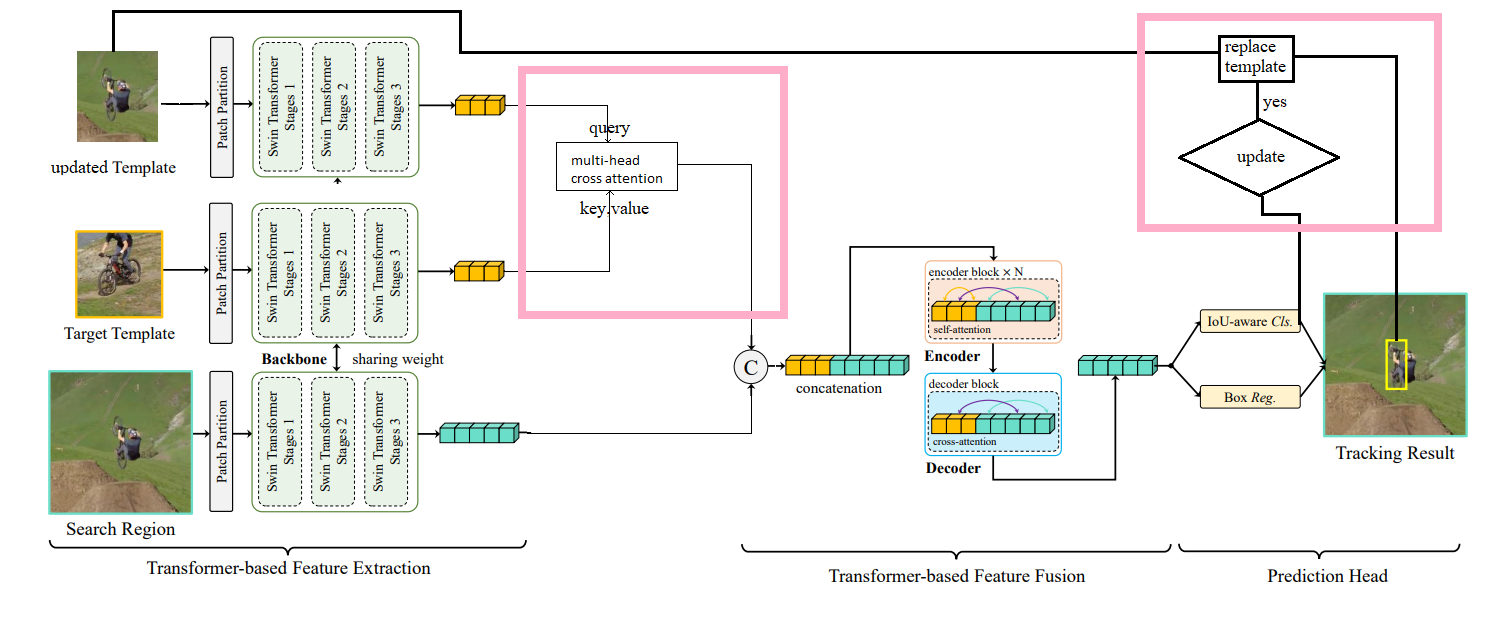
\includegraphics[width=\textwidth]{images/my_model}}
	\caption{\textRL{بنية النموذج المقترح والذي يقوم بدمج سمات صورتي الغرض عبر كتلة انتباه}}
	\label{fig:my_model}
\end{figure}
\section{خاتمة}
تحدثنا في هذا الفصل عن النموذج الأساسي في بحثنا وهو
\textLR{swinTrack}،
وبينا أن مشكلته اعتماده فقط على المعلومات المكانية، بالرغم من سرعته وتفوقه في الأداء على كثير من الملاحقات.   اعتمدنا عندها على طريقة خوارزمية
\textLR{STARK}
في إدخال المعلومات الزمانية. لذلك اقترحنا نموذج يستفيد من معلومات تغير المظهر كمعلومات زمانية، دون تغيير في بنية النموذج الأصلي، للاستفادة من أوزانه في عملية التدريب. وبما أن هذا التعديل قد حسن من أداء 
\textLR{STARK}
فقد توقعنا في بداية مرحلة البحث أنه سيحسن أداء 
\textLR{SwinTrack}.

\chapter{الاختبارات والنتائج}
\section{مقدمة}
في هذا الفصل سنتحدث عن مجموعة معطيات التدريب والاختبار وهي
\textLR{GOT-10k}،
وعن معايير التقييم والمقارنة الخاصة بهذه المجموعة، ومن ثم سنعرض نتائج تدريب كتلة الانتباه المضافة الخاصة بدمج السمات، ونعرض نتائج الاختبار على مجموعتي الـ
\textLR{validation,testing}.
ونعرض المقارنة بين الخوارزمية الأساسية 
\textLR{SwinTrack-Tiny}
وبين نموذجنا من حيث الأداء والسرعة والحجم.
\section{مجموعة معطيات التدريب 
	\textLR{\cite{got10k}GOT-10k}
}
اخترنا تدريب النموذج على مجموعة معطيات التدريب 
\textLR{GOT-10k}
الخاصة بعملية الملاحقة.
وهي اختصار لـ
\textLR{Generic Object Tracking GOT}،
تتكون من أكثر من 
$10000$
فيديو، لذلك سميت بـ
\textLR{GOT-10k}.
وتحوي أكثر من 
$105$
مليون مستطيل محيط محدد بشكل يدوي، بحجم ملف أكثر من 
$60GB$.
\newline
هذه الفيديوهات مقسمة إلى 
$563$
صنف من الأغراض، وإلى 
$87$
صنف من أنماط الحركة. وذلك بهدف تغطية أكبر قدر ممكن من تحديات الملاحقة الواقعية.
يوضح الشكل 
\ref{fig:got10k}
بعض من عينات مجموعة المعطيات 
\textLR{GOT-10k}.
\newline
أما الشكل 
\ref{fig:got10k-classes}
فيعبر عن عدد أصناف الأغراض في مجموعات التدريب الخاصة بالملاحقة، نلاحظ أن مجموعة المعطيات
\textLR{GOT-10k}
هي المعطيات الأكثر تنوعا ($563$ غرض)، يليها مجموعة معطيات 
\textLR{LaSOT\cite{Lasot}}
($70$ غرض).
\newline
توفر مجموعة المعطيات $5$ ملفات مع كل فيديو
\begin{itemize}
\item \textLR{groundtruth.txt}:
تحتوي على إحداثيات الزاوية العليا اليمينية من المستطيل المحيط، بالإضافة إلى أبعاد المستطيل.
\item \textLR{absence.label}:
القيمة $0$ تعبر عن وجود الغرض في الصورة، القيمة $1$ تعبر عن عدم وجود الغرض.
\item \textLR{cover.label}:
نسبة ظهور الهدف في الصورة،
$Value_{cover} \in \{0,1,2,...,8\}$
حيث تعبر القيمة $0$ عن غياب الغرض تماماً، وتعبر القيمة $8$ عن ظهور الهدف بشكل كامل.
\item \textLR{cut$\_$by$\_$image.label}:
حيث تعبر القيمة
$1$ عن وجود جزء من الغرض خارج نطاق الصورة،و تعبر القيمة $0$ عن وجود  كامل الغرض داخل نطاق الصورة.  
\item \textLR{meta$\_$info.ini}:
يحوي هذا الملف على رابط الفيديو، طوله، تردده، صنف الغرض، صنف الحركة، دقة الصورة.
\end{itemize}

\begin{figure}[H]
	\centerline{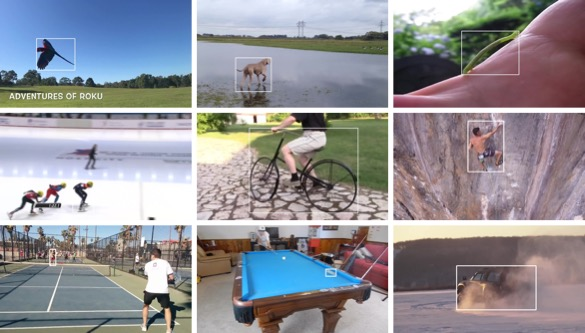
\includegraphics[width=\textwidth]{images/got10k}}
	\caption{
		\textRL{عينات من مجموعة المعطيات}
		\textLR{GOT-10k}
		\textLR{\cite{got10k}}}
	\label{fig:got10k}
\end{figure}
\begin{figure}[H]
	\centerline{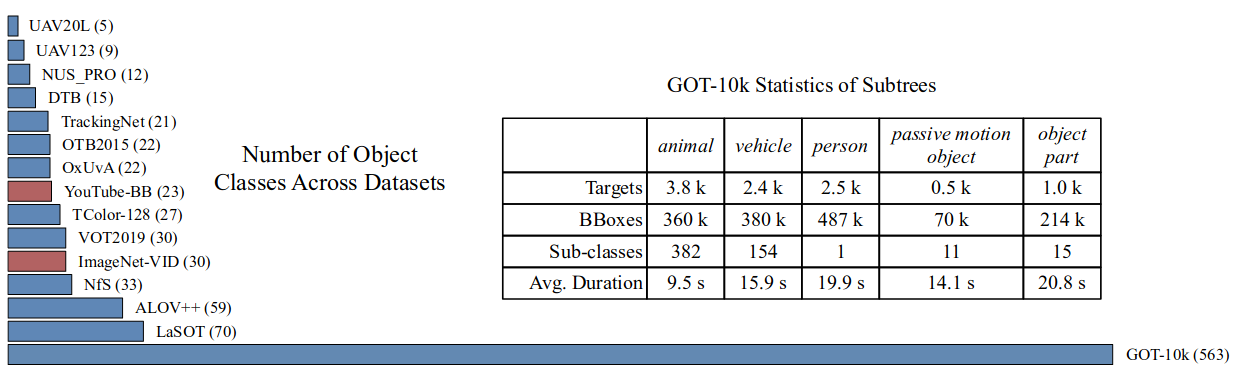
\includegraphics[width=\textwidth]{images/got10k_classes}}
	\caption{
		\textRL{عدد أصناف الأغراض في مجموعات المعطيات الخاصة بالملاحقة}
		\textLR{\cite{got10k}}}
	\label{fig:got10k-classes}
\end{figure}

هذا التصنيف لمجموعة المعطيات يفيد في تطوير خوارزميات الملاحقة، وفي إيجاد نقاط الضعف، كتحديد الحالات التي لا يستطيع فيها النموذج ملاحقة الغرض.
\subsection{معطيات الاختبار
\label{section:got10k}}
تستخدم مجموعة المعطيات
\textLR{GOT-10k}
بروتوكول
\textLR{one-shot}،
أي أنه لا يوجد تقاطع بين معطيات التدريب ومعطيات الاختبار من حيث صنف الغرض، باستثناء غرض $"$الشخص$"$.
\newline
يوضح الشكل 
\ref{fig:got10k_split}
عدد الأصناف وعدد الفيديوهات في كل مجموعة، حيث تحتوي مجموعة الاختبار على $420$ فيديو، تتألف من $84$ صنف من الأغراض، و$31$ صنف حركة.
\begin{figure}[!h]
	\centerline{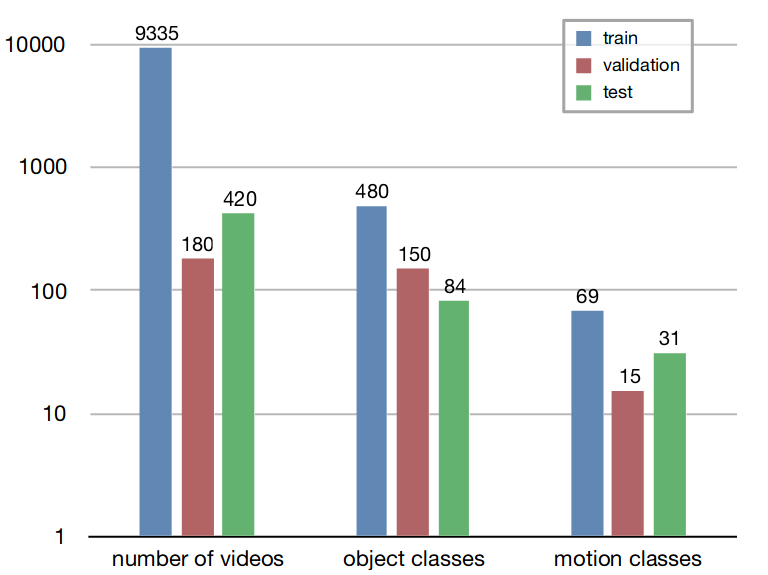
\includegraphics[scale=0.4]{images/got10k_split}}
	\caption{
		\textRL{عدد أصناف الأغراض والحركة في كل جزء من مجموعة  }
		\textLR{GOT-10k}
		\textLR{\cite{got10k}}}
	\label{fig:got10k_split}
\end{figure}
\newline
إن مجموعة الاختبار غير مزودة بالقيم الحقيقية للمستطيل المحيط، وذلك لتجنب معايرة أوزان النموذج من أجل هذه المعطيات.
لاختبار نموذج الملاحقة، نولد ملف بإحداثيات المستطيل المحيط بالهدف، هذه الاحداثيات مقدرة من قبل النموذج، ونرسله إلى مخدم خاص بمجموعة المعطيات
\textLR{GOT-10k}،
 كما يوضح الشكل
\ref{fig:got10k_submit}،
\begin{figure}[!h]
	\centerline{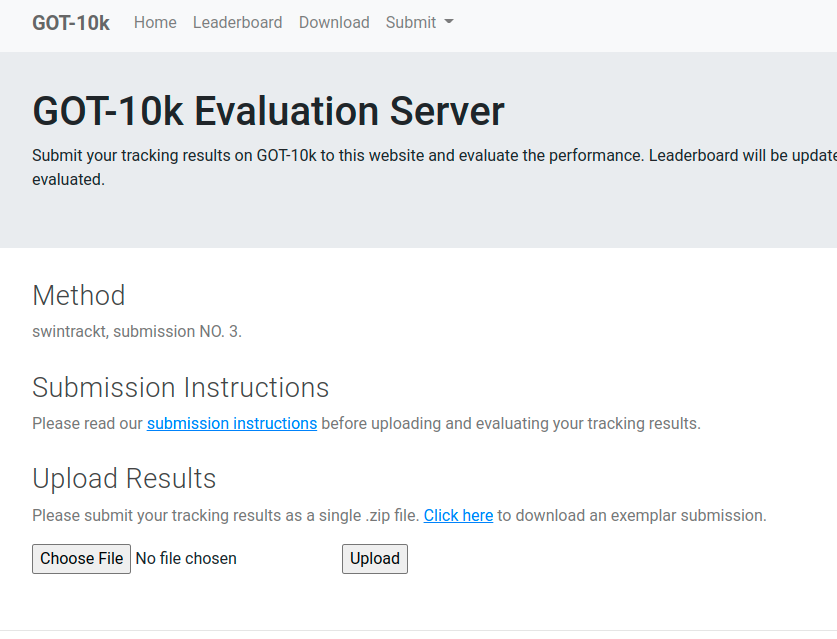
\includegraphics[width=\textwidth]{images/got10k_submit}}
	\caption{
		\begin{footnotesize}
		\textRL{المخدم الخاص بعملية اختبار الملاحق من أجل مجموعة المعطيات}
		\textLR{GOT-10k}
		\textLR{\cite{got10k}}
		\end{footnotesize}
	}
	\label{fig:got10k_submit}
\end{figure}
حيث يمتلك هذا المخدم القيم الحقيقية ويقارنها بالقيم المرسلة، ومن ثم يحسب كل من المعياريين
$mAO,mSR$
كما في الشكل
\ref{fig:got10k_result_mai}.
\newline
لمنع استخدام المخدم للتدريب أو لتعديل أوزان النموذج بحسب نتائج الأداء، فإنه لا يسمح بإرسال أكثر من ملف خلال $48$ ساعة.
\begin{figure}[!h]
	\centerline{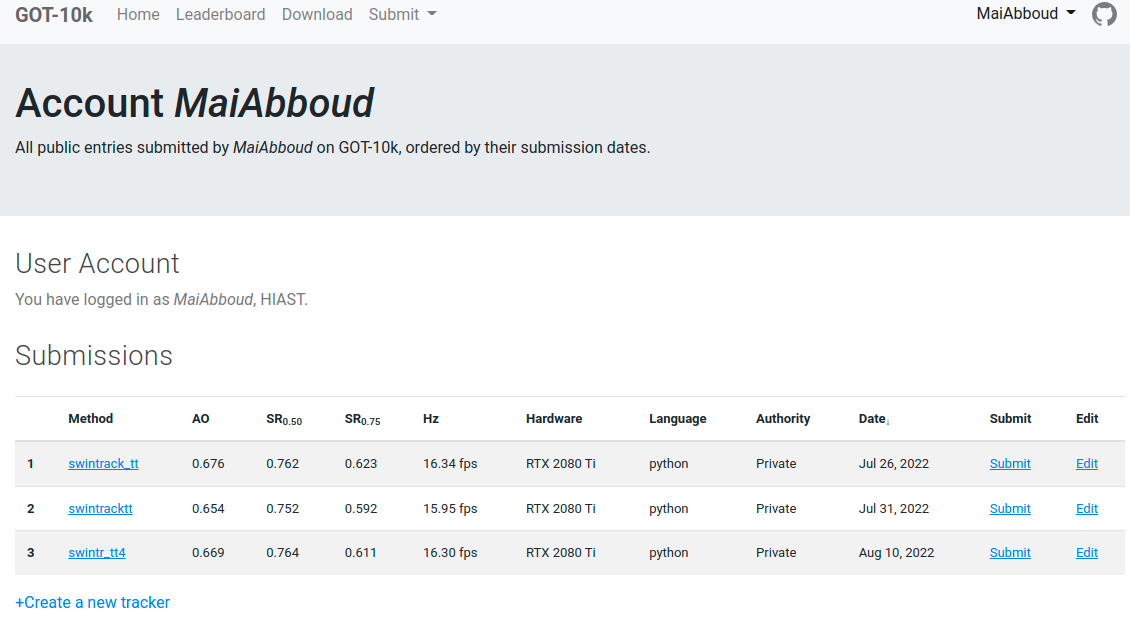
\includegraphics[width=\textwidth]{images/got10k_result_mai}}
	\caption{
		\begin{footnotesize}
		\textRL{مثال عن نتائج اختبار بعض خوارزميات الملاحقة من أجل مجموعة المعطيات}
		\textLR{GOT-10k}
		\end{footnotesize}
	}
	\label{fig:got10k_result_mai}
\end{figure}
\subsection{معايير التقييم
\textLR{Benchmarks}
\label{section:benchmark}
}
لمقارنة الملاحقات ببعضها لابد من وجود معايير لتقييم الأداء، هذه المعايير تختلف بين مجموعات المعطيات، لذلك سنذكر فقط المعايير الخاصة بمجموعة 
\textLR{GOT-10k}.
\subsubsection{المعيار الأول
\textLR{Average Overlape AO}}
يمكن تعريف 
\textLR{AO}
بأنها نسبة التقاطع إلى الاجتماع
\textLR{Intersection Over Union IOU}،
كما في الشكل
\ref{fig:iou}، 
فهي نسبة تقاطع المستطيل المحيط الحقيقي مع المستطيل المحيط المقدر من قبل الملاحق إلى إجتماع هذين المستطيلين.
\newline
\begin{figure}[H]
	\centerline{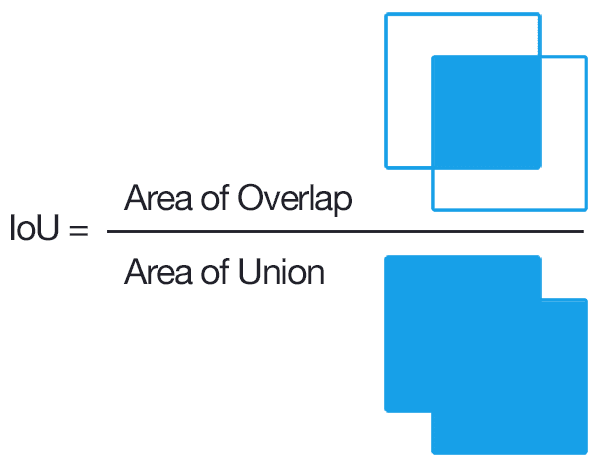
\includegraphics[scale=0.25]{images/iou_equation}}
	\caption{
		\textRL{شكل توضيحي عن }
		\textLR{IOU}
		\textLR{\cite{web:IOU_fig}}}
	\label{fig:iou}
\end{figure}
بعد الانتهاء من التدريب، ومن أجل كل 
\textLR{epoch}،
يتم اختبار النموذج بدايةً على مجموعة الـ 
\textLR{validation}.
ويتم حساب 
\textLR{mAO}،
وهي متوسط 
\textLR{AO}
من أجل كل صنف وذلك بحسب المعادلة
\begin{equation}
mAO = \frac{1}{C} \Sigma_{c=1}^C(\frac{1}{|S_c|} \Sigma_{i \in S_c}AO_i)
\end{equation}
حيث $c$ رقم الصف، $C$ عدد الصفوف، $S_c$ مجموعة الفيديوهات التي تنتمي إلى الصف $c$،
 $|S_c|$
عدد عناصر المجموعة.
\subsubsection{المعيار الثاني - معدل النجاح
\textLR{Success Rate $SR_{ratio}$}}
تقيس هذه القيمة نسبة الإطارات التي تم ملاحقتها وكان الـ
$AO$
لها
أكبر من نسبة معينة.
في معظم الأحيان يتم اظهار النتائج من أجل النسبتين 
$0.75،0.5$.
وكما في 
\textLR{AO}
فإنه يتم حساب 
$mSR_{0.75},mSR_{0.5}$
من أجل مجموعة الـ
\textLR{validation}.
\subsubsection{منحنيات التقييم - منحني النجاح 
\textLR{Success Curve}}
تعبر كل نقطة من هذه المنحني عن نسبة النجاح من أجل نسبة معينة
$threshold$،
أي التي يتجاوز فيها 
\textLR{AO}
نسبة معينة
\textLR{overlap threshold}،
كما يوضح الشكل
\ref{fig:got10k_SuccessCurve}
من أجل مجموعة من خوارزميات الملاحقة،
\begin{figure}[!h]
	\centerline{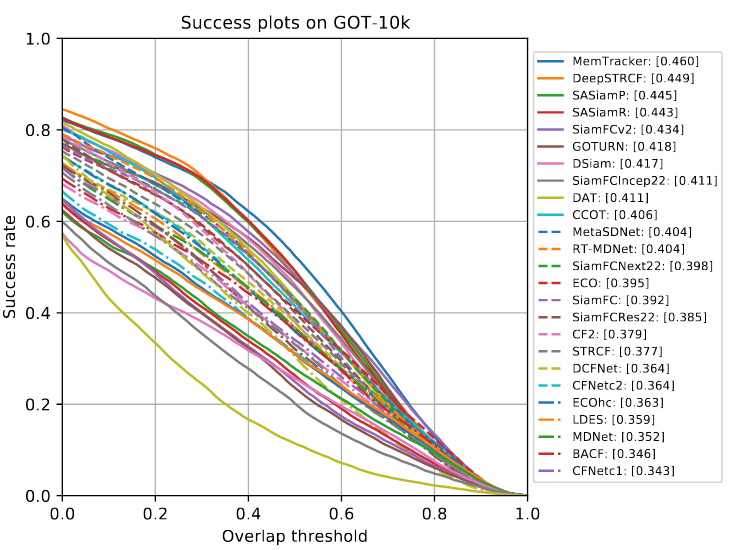
\includegraphics[width=\textwidth]{images/got10k_SuccessCurve}}
	\caption{
		\textRL{منحني النجاج من أجل عدة خوارزميات ملاحقة}
		\textLR{\cite{got10k}}}
	\label{fig:got10k_SuccessCurve}
\end{figure}
يعبر هذا المنحني من أجل القيم الصغيرة للـ
\textLR{overlap threshold}
عن الصلادة، أي عن نسبة الإطارات التي تم ملاحقتها، ومن أجل القيم الكبيرة للـ
\textLR{overlap threshold}
عن الدقة في الملاحقة.
\subsubsection{منحنيات التقييم - منحني الدقة 
	\textLR{Precision Curve}}
يعبر منحني الدقة في كل نقطة منه عن نسبة الإطارات التي بعد مركز الغرض المقدّر عن القيمة الحقيقة أقل من حد معين.
\section{النتائج}
في هذه الفقرة سنعرض نتائج النموذج الأساسي 
\textLR{SwinTrack-Tiny}،
ونتائج التجارب التي قمنا بها.
\subsection{النموذج الأساسي
\textLR{SwinTrack-Tiny}}
كما ذكرنا فإن النموذج الأساسي في بحثنا هو
\textLR{SwinTrack\cite{swinTrack}}،
وجميع اختباراتنا في الوقت الحالي هي من أجل النموذج
\textLR{SwinTrack-Tiny}،
الذي يستخدم 
\textLR{SwinTransformer-Tiny}
كـ
\textLR{backbone}،
واستخدمنا أوزان النموذج المدرب مسبقاً
على مجموعة المعطيات 
\textLR{GOT-10k}
فقط.
\subsection{التدريب}
تم تدريب النموذج من أجل إضافة كتلة انتباه ذاتي لدمج سمات الـ 
\textLR{template}
الابتدائي مع الـ
\textLR{template}
الجديد كما ذكرنا سابقاً .
سنذكر في هذا الفصل نتائج التدريب والاختبار لتجربتين.
في كلتا التجربتين أثناء مرحلة التدريب، يتم اختيار كل من الـ 
\textLR{template}
الابتدائي والـ
\textLR{template}
الجديد ونافذة البحث بشكل عشوائي من القيم الحقيقية لمجموعة التدريب من ضمن الفيديو الواحد، كما في خوارزمية
\textLR{STARK\cite{Stark}}.
\newline
\subsection{التجربة الأولى}
اخترنا بداية تجريب كتلة انتباه تقاطعي بأربع رؤوس
$h = 4$.
تم استخدام أوزان النموذج الأساسي المدرب مسبقاً على مجموعة التدريب 
\textLR{GOT-10k\cite{got10k}}
فقط، والموجودة في 
\textLR{google drive\cite{swinTrackWeights}}.
وتم التدريب بتجميد هذه الأوزان وتعديل أوزان كتلة الانتباه الذاتي المضافة فقط، 
تم التدريب باستخدام وحدة معالجة الرسومات 
\textLR{GPU NVIDIA GeForce 2080 Ti}،
واختيار 
\textLR{Epoches = 40, Batch size = 32}.
من أجل كل
\textLR{epoch}
يتم التدريب على 
$131072$ 
عينة من مجموعة التدريب.
\subsubsection{نتائج تدريب التجربة الأولى}
لتوليد منحنيات الخطأ وتتبع أداء النظام أثناء التدريب استعنا بمكتبة
\textLR{Wandb}.
حيث يبين الشكل 
\ref{chart:epoch1}
رقم العينة على المحور الأفقي، بينما رقم الـ
\textLR{epoch}
على المحور العمودي.
ويبين الشكل 
\ref{chart:lr1}
قيم معدل التدريب 
\textLR{learning rate}
أثناء عملية التدريب. 
\newline
أما كل من الأشكال
\ref{chart:loss_varifocal1},\ref{chart:loss_iou1},\ref{chart:loss1}
فهي تعبر عن تغير توابع الخطأ الممثلة في المعادلات
\ref{eq:vlclass},\ref{eq:vlregress}.
إذ نلاحظ هبوط منحنيات وسطي الخطأ، وذلك بسبب تغيير أوزان النموذج أثناء تدريبه على مجموعة المعطيات.

 \begin{figure}[H]
 	\centerline{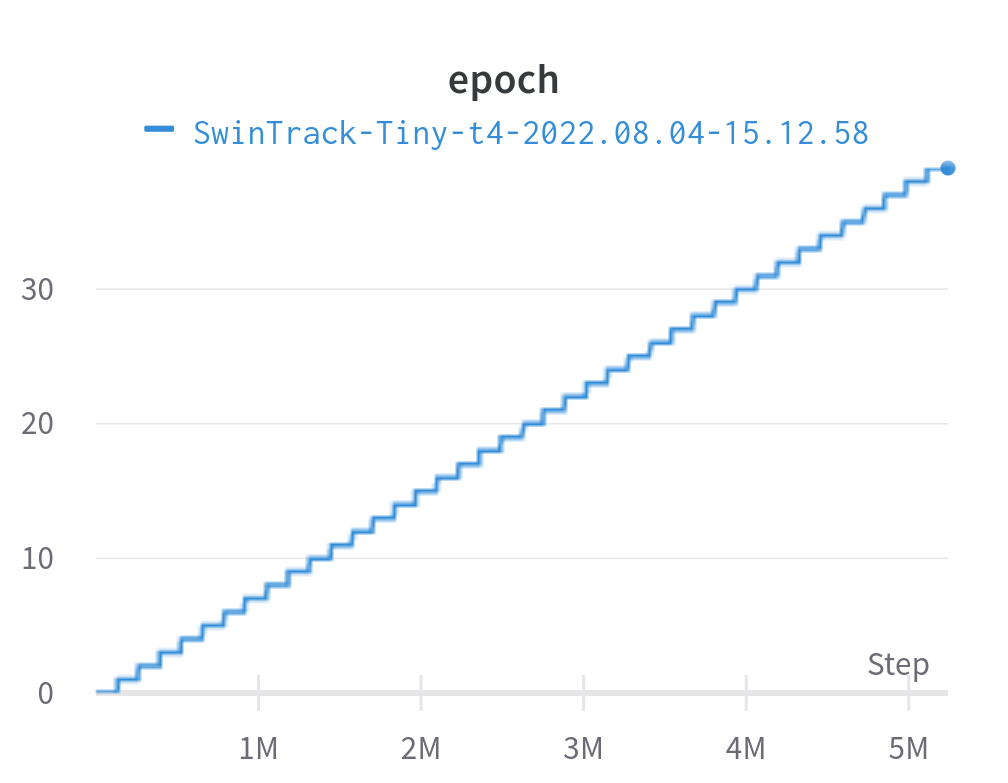
\includegraphics[width=0.7\textwidth]{charts/Section-2-Panel-6-m8q6253z0}}
 	\caption{
 		\textRL{رقم الـ}
 		\textLR{epoch}
 		\textRL{كتابع لرقم  عينة التدريب}}
 	\label{chart:epoch1}
 \end{figure}
  \begin{figure}[H]
 	\centerline{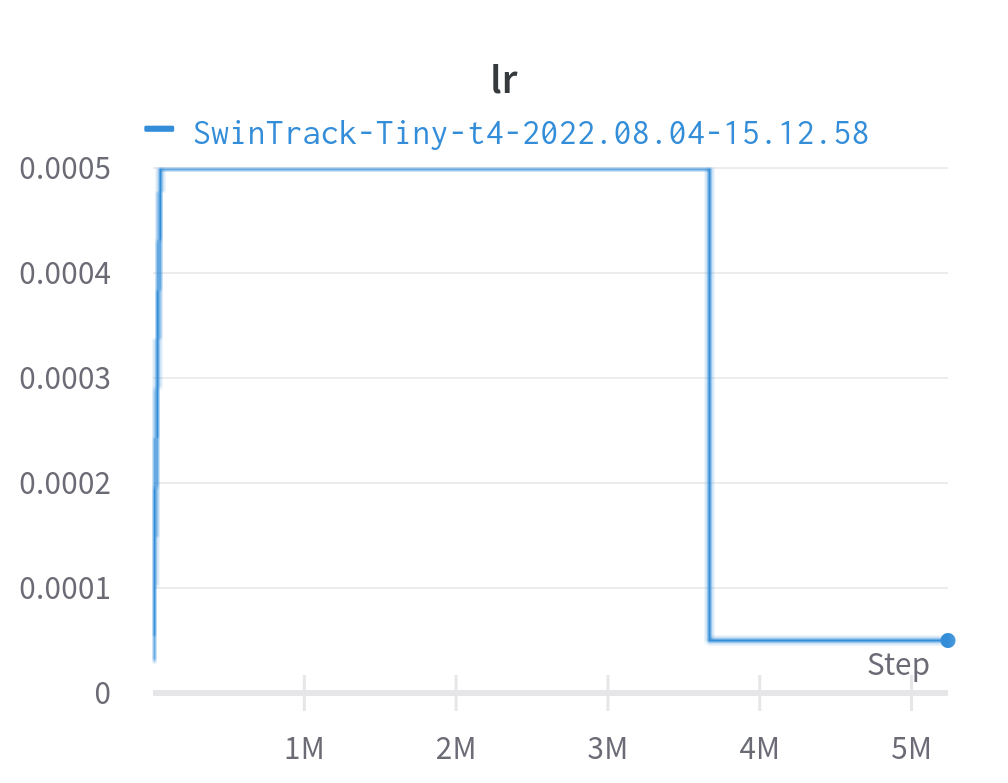
\includegraphics[width=0.7\textwidth]{charts/Section-2-Panel-12-bzoemlec5}}
 	\caption{
 		\textRL{معدل التدريب كتابع لرقم  عينة التدريب}}
 	\label{chart:lr1}
 \end{figure}

\begin{figure}[H]
	\centerline{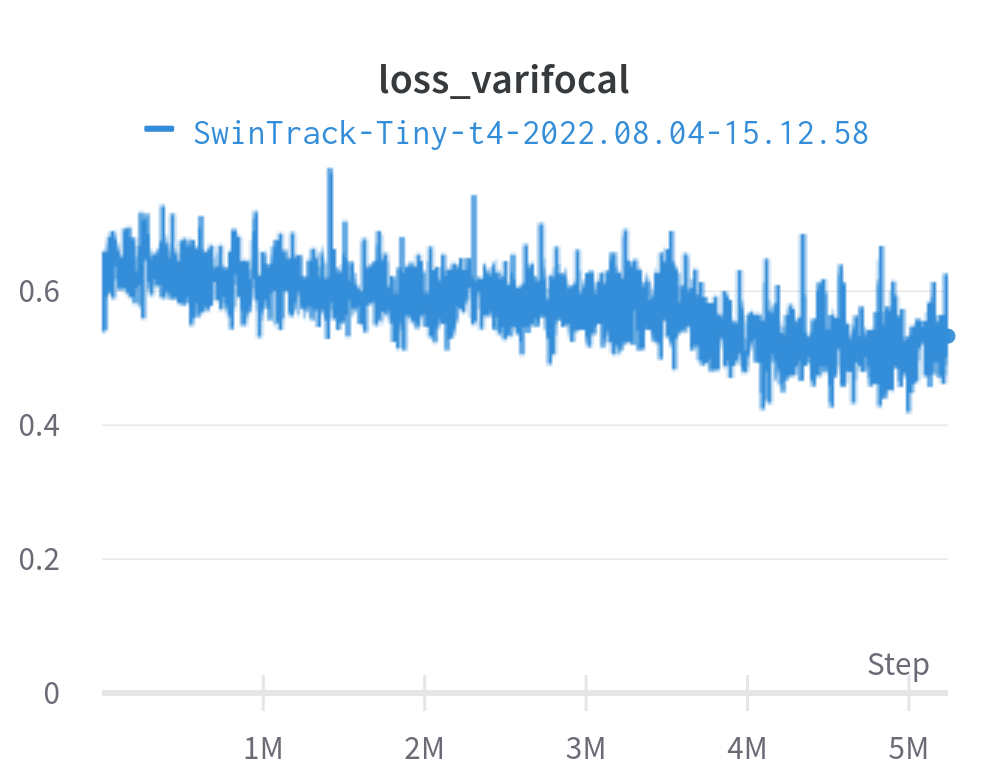
\includegraphics[width=0.7\textwidth]{charts/Section-2-Panel-9-8yjlirrqx}}
	\caption{
		\textRL{تابع خطأ شبكة التصنيف أثناء التدريب}
	}
	\label{chart:loss_varifocal1}
\end{figure}

\begin{figure}[H]
	\centerline{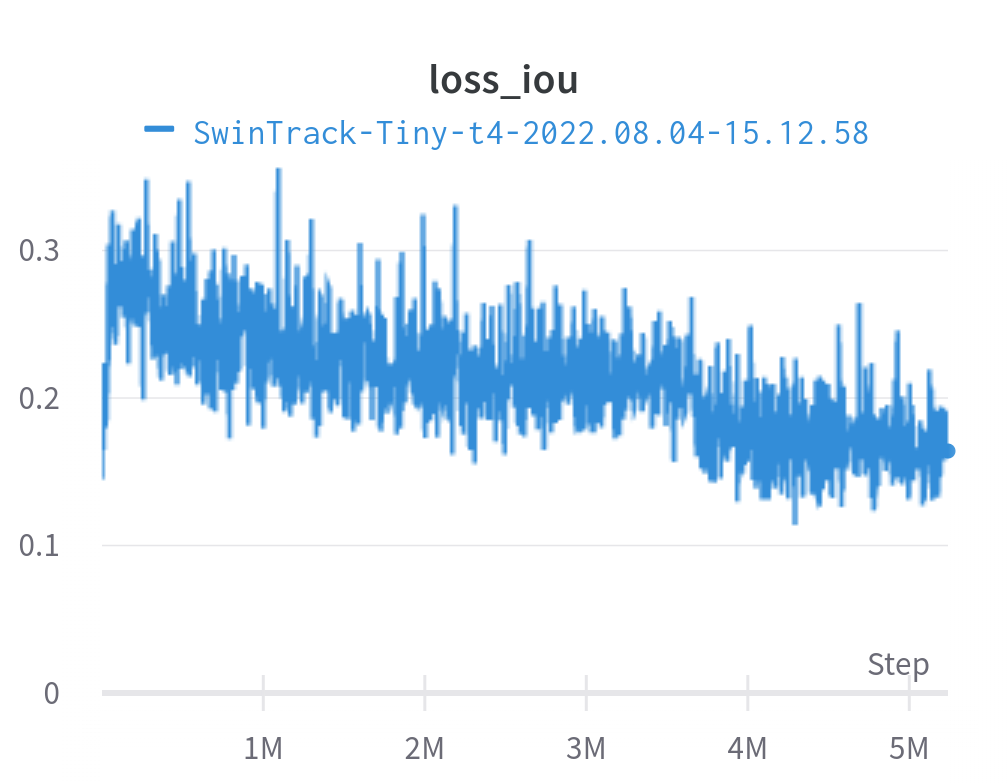
\includegraphics[width=0.7\textwidth]{charts/Section-2-Panel-13-ffs6mrffa}}
	\caption{
		\textRL{تابع خطأ شبكة الـ}
		\textLR{regression}
		\textRL{أثناء التدريب}
	}
	\label{chart:loss_iou1}
\end{figure}

\begin{figure}[H]
	\centerline{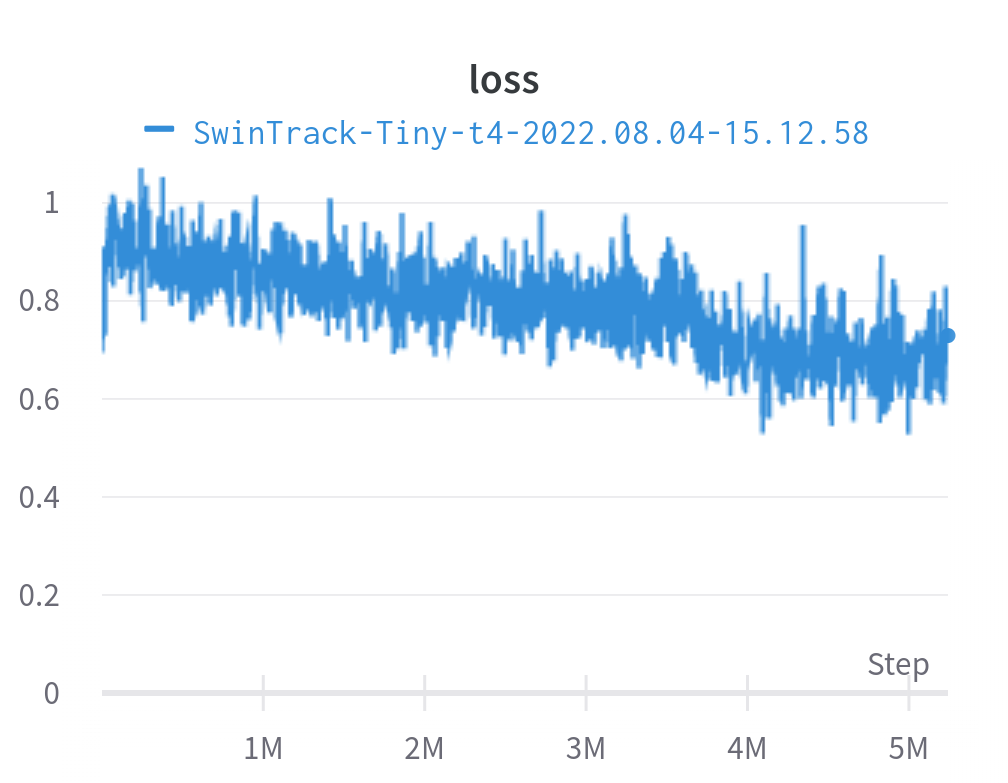
\includegraphics[width=0.7\textwidth]{charts/Section-2-Panel-11-jg4qpu2ty}}
	\caption{
		\textRL{تابع الخطأ الكلي أثناء التدريب}
	}
	\label{chart:loss1}
\end{figure}
\subsubsection{ نتائج التجربة الأولى على مجموعة الـ
\textLR{validation}}
يتم اختبار النموذج على مجموعة الـ
\textLR{validation}
بعد كل 
\textLR{epoch}
وذلك أثناء عملية التدريب.
تبين الأشكال
\ref{chart:val_loss_varifocal},\ref{chart:val_loss_iou},\ref{chart:val_loss}
منحنيات الخطأ لشبكتي التصنيف والـ
\textLR{regression}،
ومنحني الخطأ الكلي.
وكما في منحنيات وسطي الخطأ أثناء التدريب، فإن وسطي خطأ النموذج على معطيات الـ
\textLR{validation} 
في تناقص بعد كل 
\textLR{epoch}.
\begin{figure}[H]
	\centerline{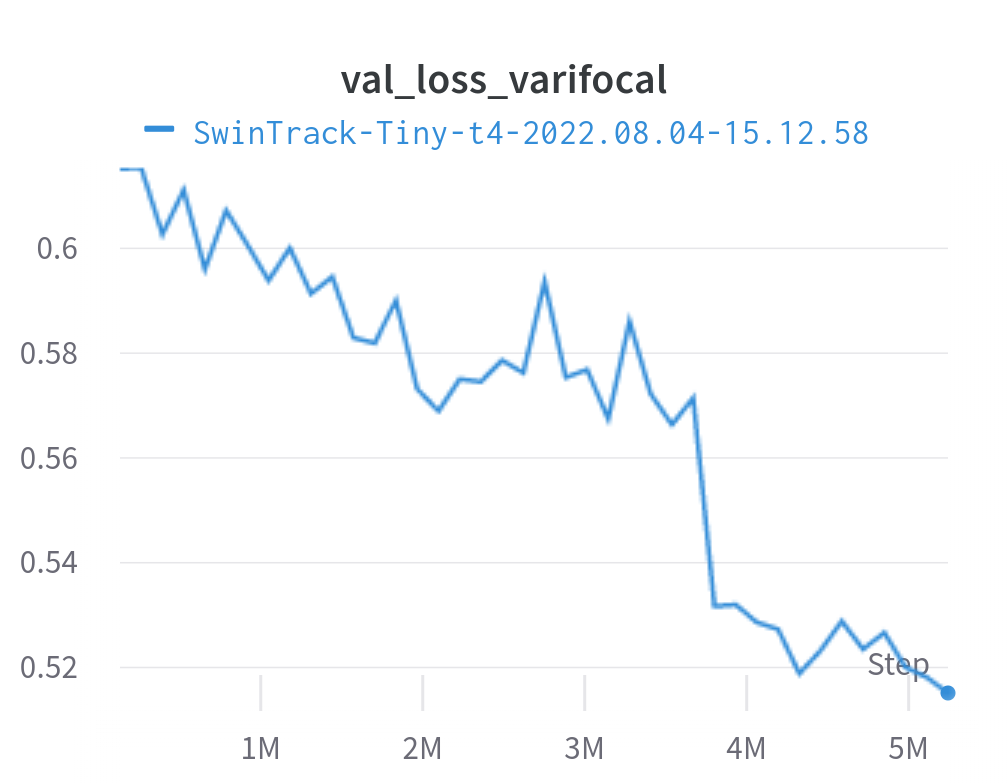
\includegraphics[width=0.7\textwidth]{charts/Section-2-Panel-1-5x2brafi7}}
	\caption{
		\textRL{خطأ شبكة التصنيف على مجموعة الـ}
		\textLR{validation}
	}
	\label{chart:val_loss_varifocal}
\end{figure}

\begin{figure}[H]
	\centerline{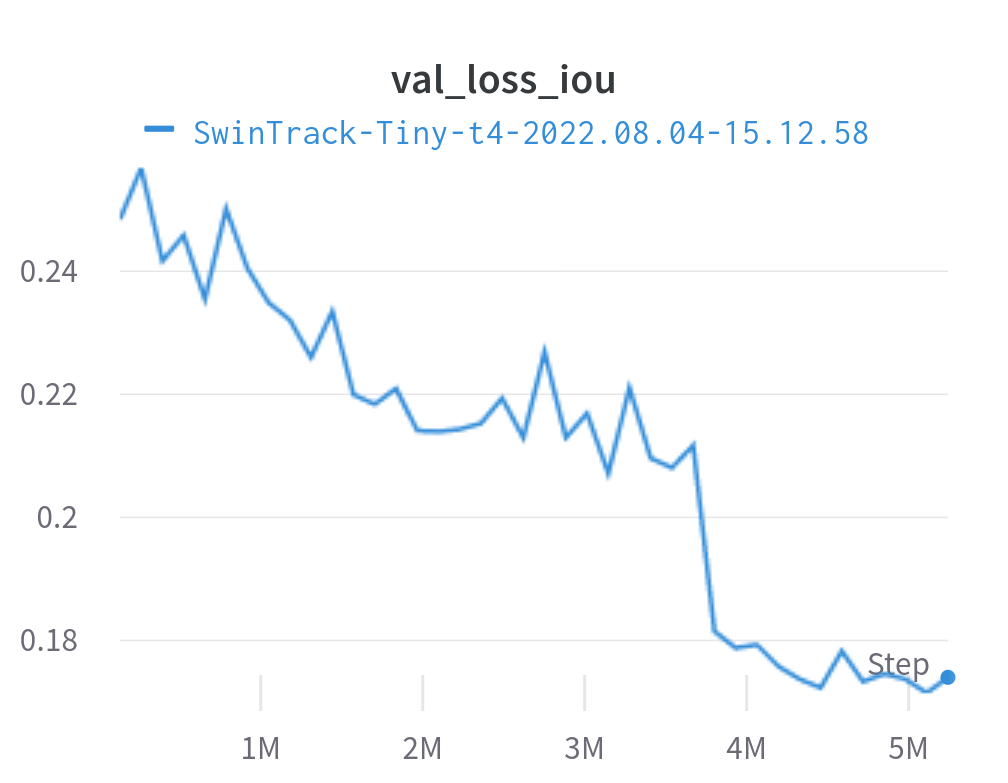
\includegraphics[width=0.7\textwidth]{charts/Section-2-Panel-2-owiohngs7}}
	\caption{
		\textRL{تابع خطأ شبكة الـ}
		\textLR{regression}
		\textRL{على مجموعة الـ}
		\textLR{validation}
	}
	\label{chart:val_loss_iou}
\end{figure}

\begin{figure}[H]
	\centerline{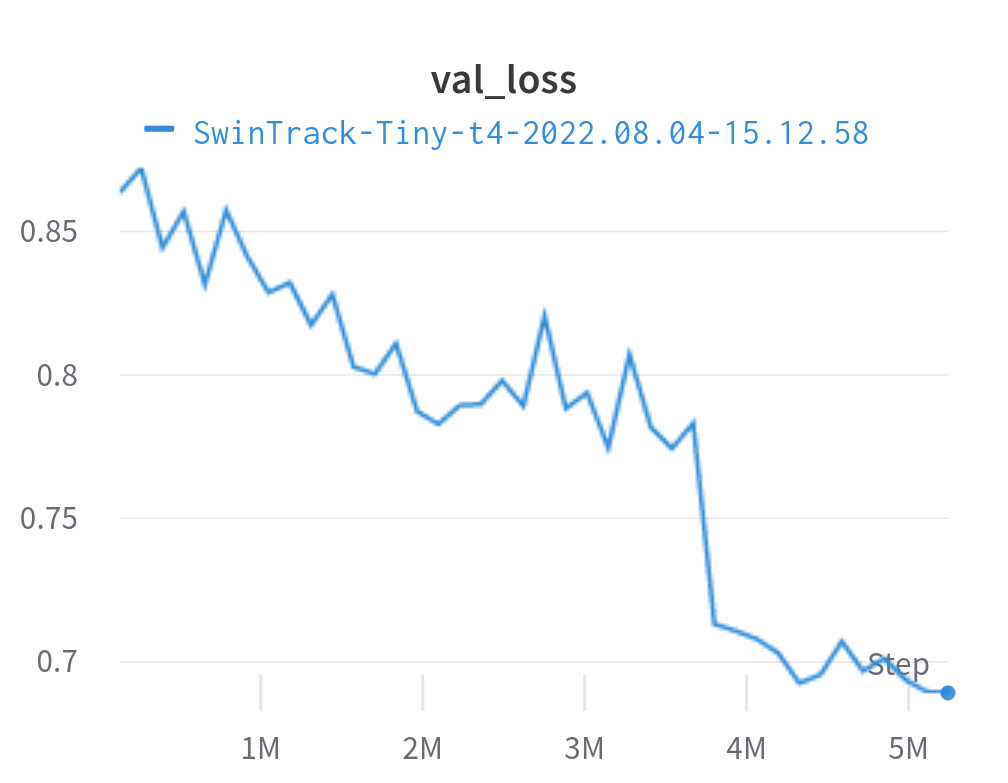
\includegraphics[width=0.7\textwidth]{charts/Section-2-Panel-0-jvrhhrv9d}}
	\caption{
		\textRL{تابع الخطأ الكلي على مجموعة الـ}
		\textLR{validation}
	}
	\label{chart:val_loss}
\end{figure}

%\subsubsection{أداء النظام أثناء التجربة الأولى}
%\selectlanguage{english}
%\begin{figure}[H]
%	\minipage{0.49\textwidth}
%	\includegraphics[width=0.7\linewidth]{charts/Section-4-Panel-10-ez7r8q2s1}
%	\caption{\textRL{أثناء التدريب}
%		GPU
%		\textRL{درجة حرارة الـ}}
%	\endminipage\hfill
%	\minipage{0.49\textwidth}
%	\includegraphics[width=0.7\linewidth]{charts/Section-4-Panel-11-7ugto7ti8}
%	\caption{
%		\textRL{أثناء التدريب}
%		GPU
%		\textRL{نسبة استخدم الـ}}
%	\endminipage
%\end{figure}
%\begin{figure}[H]
%	\minipage{0.49\textwidth}
%	\includegraphics[width=0.7\linewidth]{charts/Section-4-Panel-6-0i8v5s4ys}
%	\caption{GPU
%		\textRL{نسبة استهلاك الطاقة للـ}}
%	\endminipage\hfill
%\end{figure}
%\selectlanguage{arabic}
\subsection{التجربة الثانية}
تم تجريب كتلة انتباه تقاطعي بثمانية رؤوس
$h = 8$.
مع استخدام أوزان النموذج المدرب في التجربة الأولى كأوزان ابتدائية، وأثناء التدريب تم تجميد الأوزان ما عدا أوزان كتلة الانتباه.
تم التدريب عن طريق وحدة معالجة الرسومات 
\textLR{GPU NVIDIA GeForce 3060 Ti}
واختيار 
\textLR{Epoches = 9 , Batch size=1}.
\subsection{عرض ومناقشة النتائح}
سنعرض في هذه الفقرة نتائج اختبار النموذج من أجل التجربتين السابقتين على مجموعة الـ
\textLR{validation}،
وعلى مجموعة الاختبار 
\textLR{testing}.
وبما أننا لا نملك القيم الحقيقية لمجموعة الاختبار، وبما أن مجموعة الاختبار لا تتقاطع مع مجموعتي التدريب والـ 
\textLR{validation}
من حيث صنف الغرض، فسيكون تقييم النموذج على مجموعة الاختبار هو الأكثر أهمية، لأنه يعبر عن قدرة النموذج على التعميم.
\newline
يوضح الجدول
\ref{table:my_model_compare_val}
نتائج الاختبار على مجموعة الـ
\textLR{validation}
الخاصة بـ
\textLR{GOT-10k}،
وذلك من أجل الخوارزمية الأساسية 
\textLR{SwinTrack-Tiny\cite{swinTrack}}،
ومن أجل التجربتين الموضحتين سابقاَ. وبما أننا أضفنا تابع انتباه بأربع رؤوس مع إضافة معلومات زمانية فرمزنا للنموذج في التجربة الأولى بـ
\textLR{SwinTrack-t4}.
ولنموذج التجربة الثانية بـ 
\textLR{SwinTrack-t8}،
كوننا استخدمنا تابع انتباه بثمانية
$8$
رؤوس.
\newline
أما الجدول 
\ref{table:my_model_compare_test}
فيوضح نتائج اختبار الخوارزميات السابقة على مجموعة الاختبار 
\textLR{testing}.
%\selectlanguage{english}
\begin{table}[H]
	\centering
	\begin{tabular}{c |c| c |c} 
		\hline
		& \textLR{SwinTrack-Tiny} & \textLR{SwinTrack-t4} & \textLR{SwinTrack-t8}\\[0.5ex] 
		\hline\hline
		$AO$ & $69.6$& $70.4$&$69.8$\\
		$SR_{0.50}$ &$79.5$&$81.1$&$80.3$\\ 
		$SR_{0.75}$ &$64.8$&$63.2$&$63.6$\\
		$Hz$ &&&\\[1ex] 
		\hline
	\end{tabular}
	\caption{\textRL{نتائج اختبار  النماذج من أجل مجموعة}
	\textLR{testing-GOT-10k}}
	\label{table:my_model_compare_test}
\end{table}

\begin{table}[H]
	\centering
	\begin{tabular}{c |c |c| c} 
		\hline
		 & \textLR{SwinTrack-Tiny} & \textLR{SwinTrack-t4} & \textLR{SwinTrack-t8}\\[0.5ex] 
		\hline\hline
		\textLR{update interval} & &$10 $&$30$\\
		\textLR{iou threshold} &&&$0.8$\\ 
		\textLR{Success Score} &$81.6$&$79.2$&$79.8$\\
		\textLR{Precision Score} &$75.1$&$71.2$&$72.3$\\
		\textLR{Normalized Precision Score} &$91.7$&$89.7$&$90.2$\\
		\textLR{Average Overlap} &$83.2$&$80.7$&$81.3$\\
		$SR_{0.5}$&$93.2$&$90.8$&$91.6$\\
		$SR_{0.75}$&$81.8$&$78.1$&$80$\\
		$FPS$&$88$&$72$&$88$\\
		\textLR{params(M)}&$22.7$&$23.3$&$23.3$\\[1ex] 
		\hline
	\end{tabular}
	\caption{\textRL{نتائج اختبار  النماذج من أجل مجموعة}
	\textLR{validation-GOT-10k}}
	\label{table:my_model_compare_val}
\end{table}


%report
\begin{table}[H]
	\centering
	\begin{tabular}{c |c |c| c} 
		\hline
		& \textLR{SwinTrack-Tiny} & \textLR{SwinTrack-t4} & \textLR{SwinTrack-t8}\\[0.5ex] 
		\hline\hline
		\textLR{update interval} & &$10 $&$30$\\
		\textLR{iou threshold} &&&$0.8$\\ 
		\textLR{Average Overlap} &$83.2$&$80.7$&$81.3$\\
		$SR_{0.5}$&$93.2$&$90.8$&$91.6$\\
		$SR_{0.75}$&$81.8$&$78.1$&$80$\\
		$FPS$&$88$&$72$&$88$\\
		\textLR{params(M)}&$22.7$&$23.3$&$23.3$\\[1ex] 
		\hline
	\end{tabular}
	\caption{\textRL{نتائج اختبار  النماذج من أجل مجموعة}
		\textLR{validation-GOT-10k}}
	\label{table:my_model_compare_val}
\end{table}


\selectlanguage{arabic}

\begin{table}[H]
	\centering
	\begin{tabular}{c |c| c |c} 
		\hline
		\textRL{النموذج}& $AO$ & $SR_{0.50}$ & $SR_{0.75}$\\[0.5ex] 
		\hline\hline
		\textLR{Ours-t4}&\textcolor{red}{$70.4$}&\textcolor{red}{$81.1$}&$63.2$\\
		\textLR{Ours-t8}&\textcolor{blue}{$69.8$}&\textcolor{blue}{$80.3$}&\textcolor{blue}{$63.6$}\\
		\textLR{SwinTrack-B}&$69.4$&$78$&\textcolor{red}{$64.3$}\\[1ex] 
		\textLR{SLT-TransT}&$67.5$&$76.8$&$60.3$\\
		\textLR{TREG}&$66.8$&$77.8$&$57.2$\\
		\textLR{Siam R-CNN}&$64.9$&$72.8$&\\
		\textLR{STMTrack}&$64.2$&$73.7$&$57.5$\\
		\textLR{Ocean}&$61.1$&$72.1$&\\
		\textLR{DiMP}&$61.1$&$71.7$&\\
		\textLR{SiamFC++}&$61.0$&$74.2$&\\
		\textLR{ATOM}&$55.6$&$63.4$&\\[1ex]
		\hline
	\end{tabular}
	\caption{\textRL{مقارنة بين عدة خوارزميات ملاحقة من أجل مجموعة}
	\textLR{testing-GOT-10k}}
	\label{table:my_model_compare_test}
\end{table}



%report
\begin{table}[H]
	\centering
	\begin{tabular}{c |c| c |c|c} 
		\hline
		\textRL{النموذج}& $AO$ & $SR_{0.50}$ & $SR_{0.75}$& \textLR{year}\\[0.5ex] 
		\hline\hline
		\textLR{Ours-t4}&\textcolor{red}{$70.4$}&\textcolor{red}{$81.1$}&$63.2$&$2022$\\
		\textLR{Ours-t8}&\textcolor{blue}{$69.8$}&\textcolor{blue}{$80.3$}&\textcolor{blue}{$63.6$}&$2022$\\
		\textLR{SwinTrack-B}&$69.4$&$78$&\textcolor{red}{$64.3$}&$2021$\\[1ex] 
		\textLR{SLT-TransT}&$67.5$&$76.8$&$60.3$&$2022$\\
		\textLR{TREG}&$66.8$&$77.8$&$57.2$&$2021$\\
		\textLR{Siam R-CNN}&$64.9$&$72.8$&&$2019$\\
		\textLR{STMTrack}&$64.2$&$73.7$&$57.5$&$2021$\\
		\textLR{Ocean}&$61.1$&$72.1$&&$2020$\\
		\textLR{DiMP}&$61.1$&$71.7$&&$2019$\\
		\textLR{SiamFC++}&$61.0$&$74.2$&&$2019$\\
		\textLR{ATOM}&$55.6$&$63.4$&&$2018$\\[1ex]
		\hline
	\end{tabular}
	\caption{\textRL{مقارنة بين عدة خوارزميات ملاحقة من أجل مجموعة}
		\textLR{testing-GOT-10k}}
	\label{table:my_model_compare_test}
\end{table}
نلاحظ من الجدول 
\ref{table:my_model_compare_val}
بمقارنة الخوارزميات السابقة من ناحية السرعة في السطر المقابل لـ 
\textLR{FPS frame by second}،
بأن كتلة الانتباه التي أضفناها مع تحديث الـ
\textLR{template}
كل 
$30$
إطار لم تؤثر على السرعة من أجل $4$ رؤوس، بينما التحديث كل 
$10$
إطارات قد خفض الزمن بمقدار 
$8FPS$
عند الاختبار من أجل
$8$
رؤوس.
ونلاحظ أيضاً أن الأداء لم يتحسن بالنسبة للاختبار على معطيات الـ
\textLR{validation}.
\newline
لكن بالمقابل 
بمقارنة الخوارزميات على مجموعة الاختبار
عن طريق المخدم الخاص بـ
\textLR{GOT-10k}،
وكما يوضحه الجدول 
\ref{table:my_model_compare_test}،
% عند اختبارها على معطيات الـ
%\textLR{testing}
%
فقد تحسن الأداء في كل من التجربتين. في التجربة الأولى
\textLR{SwinTrack-t4}
 فقد تحسنت نسبة
$AO$
بمقدار
$0.8\%$،
و
$1.6\%$
بالنسبة للمقدار
$SR_{0.5}$.
نفسر اختلاف النتائج بالنسبة لمجموعتي الاختبار والـ
\textLR{validation}،
%نفسر ذلك بأن مجموعة الـ
%\textLR{validation}
بأن مجموعة التدريب ومجموعة الـ
\textLR{validation}
تتقاطع من ناحية صنف الغرض والحركة كما ذكرنا في الفقرة
\ref{section:got10k}،
لكنها لاتتقاطع مع معطيات الاختبار.
بالإضافة إلى أن النموذج الأساسي تم تدريبه من أجل 
$Epoches = 300$
بينما نموذج اختبارنا الأول من أجل 
$Epoches = 40$،
ونموذج الاختبار الثاني من أجل 
$Epoches = 9$ 
فقط. وهذا ما يفسر 
\textLR{underfitting}
بالنسبة لمجموعة التدريب والتي مجموعة الـ
\textLR{validation}
جزء منها.
وبنفس الوقت فإن التدريب من أجل 
$epoches$
قليلة وتجميد أوزان النموذج الأساسي وتعديل أوزان كتلة الانتباه فقط، جنب النموذج المعدل الـ
\textLR{overfitting}
وهذا ما يفسر تحسن الأداء بالنسبة لمعطيات الـ
\textLR{testing}،
والتي تختلف عن معطيات التدريب والـ
\textLR{validation}.
\newline
بالنسبة للتجربة الثانية
\textLR{SwinTrack-t8}
 فإن تحسن الأداء كان بنسبة 
$0.2\%$
بالنسبة للـ
$AO$،
وبنسبة 
$0.6\%$
بالنسبة لـ
$SR_{0.5}$.
هذا التحسن الطفيف في الأداء يمكن أن نفسره بأن النموذج لم يدرب بشكل كافي، إذ تم تدريبه على 
\textLR{9 epoches}
فقط،
وذلك بسبب مشاكل تقنية في وحدة معالجة الرسومات 
\textLR{GPU NVIDIA GeForce 2080 Ti}،
لذلك لم نتمكن من تدريب النموذج الثاني عليها.
\newline
من المتوقع أن يتحسن الأداء بشكل أكبر إذا تم تدريب النموذج على عدد أكبر من الـ
$epoches$.
\newline
في كلا التجربتين نلاحظ تراجع قيمة 
$SR_{0.75}$
بمقدار 
$1.6\%$
للنموذج الأول، وبمقدار 
$1.2$
للنموذج الثاني، هذا يعني أن دقة الملاحقة أقل من النموذج الأساسي ولكن عدد الإطارات التي تتم ملاحقتها أكبر، أي أن تحديث صورة الهدف ودمجه مع الصور الابتدائية بالطريقة التي اختبرناها قد جعل الملاحق أكثر صلادة ولكن أقل دقة.
\newline
يبين الجدول 
\ref{table:many_model_compare_test}
مقارنة بين النماذج المتعلقة باختباراتنا في البحث  مع خوارزميات الملاحقة الحديثة التي تتصدر أفضل أداء بالنسبة لمجموعة المعطيات 
\textLR{GOT-10k\cite{got10k}}،
وذلك عند البدء في البحث في عام
$2022$.
\newline
أما بالنسبة لمنحنيات التقييم فيوضح الشكلان
\ref{fig:successCurve}
و
\ref{fig:precision}
منحنيات النجاح والدقة بالنسبة للنماذج الثلاثة المذكور سابقاَ، وذلك من أجل مجموعة الـ
\textLR{validation}،
حيث النموذج الأصلي 
\textLR{SwinTrack-Tiny}
باللون الأزرق، و
\textLR{SwinTrack-t4}
باللون الأخضر، أما
\textLR{SwinTrack-t8}
باللون البرتقالي.
وكما ذكرنا سابقاً فإن أداء النماذج المعدلة لم يتحسن بالنسبة لمجموعة الـ
\textLR{validation}،
وهذا مايفسر تواجد منحنيات النموذجين المعدلين
أسفل النموذج الأصلي
\textLR{SwinTrack-Tiny}
\begin{figure}[H]
	\centerline{\includegraphics[width=\textwidth]{charts/successCurve}}
	\caption{\textRL{
	\begin{footnotesize}
			منحني النجاح للنماذج الثلاثة، اللون الأزرق هو النموذج الأصلي، اللون الأخضر هو التجربة الأولى بكتلة انتباه بـ 
			$4$ 
			رؤوس، واللون البرتقالي هو التجربة الثانية بـ
			$8$
			رؤوس
	\end{footnotesize}
	}}
	\label{fig:successCurve}
\end{figure}

\begin{figure}[H]
	\centerline{\includegraphics[width=\textwidth]{charts/precision curve}}
	\caption{\textRL{منحني الدقة للنماذج الثلاثة}}
	\label{fig:precision}
\end{figure}

\subsubsection{اختبارت الخوارزميات على  الفيديو}
اختبرنا الخوارزميات السابقة على عدة فيديوهات من مجموعة الـ 
\textLR{validation}، 
وأظهرنا نتائج الملاحقة في الصور التالية، بحيث يقابل كل لون من ألوان المستطيلات إلى خوارزمية وفق مايلي:
%ألوان النماذج كمايلي
\begin{itemize}
	\item 	القيم الحقيقة باللون الأخضر
	\item
	النموذج الأصلي 
	\textLR{SwinTrack-Tiny}
	باللون الأصفر
	\item
	نموذج التجربة الأولى
	\textLR{SwinTrack-t4}
	باللون الزهري
	\item
	نموذج التجربة الثانية
	\textLR{SwinTrack-t8}
	باللون السماوي
\end{itemize}

في الشكل
\ref{fig:video_success_1}
مثال عن نجاح النماذج في الملاحقة، ولكن النموذج الأصلي بدقة أقل من النموذجين المعدلين، وذلك بسبب وجود أغراض مشابهة للغرض الملاحَق.
\begin{figure}[H]
	\centerline{\includegraphics[width=\textwidth]{images/results/success/project_52}}
	\caption{\textRL{مثال عن الملاحقة مع وجود أغراض مشابهة}}
	\label{fig:video_success_1}
\end{figure}
أيضاً بالنسبة للشكل
\ref{fig:video_success_2}
فإن النموذج الأصلي يفشل في الملاحقة، بينما النموذج المعدل حسن من الأداء في هذه الحالة.
\begin{figure}[H]
	\centerline{\includegraphics[width=\textwidth]{images/results/success/project_161}}
	\caption{\textRL{مثال عن الملاحقة مع وجود أغراض مشابهة}}
	\label{fig:video_success_2}
\end{figure}
في الشكل 
\ref{fig:video_success_3_initial}
نتيجة الملاحقة في بداية الفيديو، وعندما يتغير شكل الغرض بشكل كبير كما في الشكل 
\ref{fig:video_success_3}،
فإن النموذج الأصلي لا يستطيع أن يحدد مكان الغرض بدقة النموذجين المعدلين، وذلك كون التعديل المضاف يأخذ بعين الإعتبار التغيرات التي تطرأ على شكل الغرض، ويدخلها إلى النموذج من جديد.
\begin{figure}[H]
	\centerline{\includegraphics[width=\textwidth]{images/results/success/project_1802}}
	\caption{\textRL{مثال عن الملاحقة مع تغير كبير في شكل الغرض}}
	\label{fig:video_success_3_initial}
\end{figure}

\begin{figure}[H]
	\centerline{\includegraphics[width=\textwidth]{images/results/success/project_180}}
	\caption{\textRL{مثال عن الملاحقة مع تغير كبير في شكل الغرض}}
	\label{fig:video_success_3}
\end{figure}
أما في الشكل
	\ref{fig:video_fail_1_initial}
	فيكون المطلوب ملاحقة أغراض صغيرة، ووجود أغراض مشابهة بجوار الغرض المطلوب.
	هنا نرى في الشكل 
	\ref{fig:video_fail_1}
	فشل النموذجين المعدلين بينما ينجح النموذج الأصلي في هذه الحالة.
\begin{figure}[H]
	\centerline{\includegraphics[width=\textwidth]{images/results/failed/project_175.avi}}
	\caption{\textRL{ 
			مثال عن ملاحقة أغراض صغيرة - بداية عملية الملاحقة
	}}
	\label{fig:video_fail_1_initial}
\end{figure}

\begin{figure}[H]
	\centerline{\includegraphics[width=\textwidth]{images/results/failed/project_175.avi1}}
	\caption{\textRL{
			مثال عن ملاحقة أغراض صغيرة - أثناء عملية الملاحقة
	}}
	\label{fig:video_fail_1}
\end{figure}	
	وأيضا فيما يتعلق بالشكلين
	\ref{fig:video_fail_2_initial}
		و
	\ref{fig:video_fail_2}.
	نستنتج من الفيديوهات السابقة أن التعديل قد حسن من الأداء من أجل الأغراض التي يتغير مظهرها بشكل كبير، لكن ليس من أجل الأغراض الصغيرة أو في حالة وجود أغراض مشابهة للغرض المطلوب ملاحقته.
	هنا يمكن تفسير ذلك بأن النموذجين المعدلين مدربان على أخذ تغير مظهر الغرض بعين الاعتبار، وبالتالي عند وجود أغراض مشابهة فإنه لايستطيع التمييز بينها وبين الغرض المطلوب ملاحقته في أثناء تغير مظهره.
\begin{figure}[H]
	\centerline{\includegraphics[width=\textwidth]{images/results/failed/project_129.avi2}}
	\caption{\textRL{مثال عن الملاحقة مع وجود أغراض مشابهة}}
	\label{fig:video_fail_2_initial}
\end{figure}

\begin{figure}[H]
	\centerline{\includegraphics[width=\textwidth]{images/results/failed/project_129.avi3}}
	\caption{\textRL{مثال عن الملاحقة مع وجود أغراض مشابهة}}
	\label{fig:video_fail_2}
\end{figure}

%\chapter{الخاتمة والآفاق المستقبلية}
\section{الخاتمة}
قمنا في هذا البحث بالتعرف على أنواع الملاحقة، وبالتركيز على الملاحقات التي تستخدم تقنيات التعلم العميق، وبالتعرف على نموذج المحول وعلى التابع الأساسي فيه وهو تابع الانتباه، كما أننا ذكرنا تطبيقات المحول في مجال الرؤية الحاسوبية، وركزنا على تطبيقاته في مجال الملاحقة.
وبما أن النموذج الأساسي في البحث هو 
\textLR{SwinTrack} 
والذي يستخدم محول 
\textLR{Swin}
لاستخلاص السمات، لذلك قمنا بشرح مفصل عن هذا المحول، وسبب ملائمته لتطبيقات الرؤية الصنعية وللزمن الحقيقي.
ثم شرحنا عن النموذج الأساسي
\textLR{SwinTrack-Tiny} 
وسبب اختيارنا له، وكونه يستخدم فقط المعلومات المكانية، لذلك كانت فكرة التعديل هي باستخدام المعلومات الزمانية وذلك عن طريق إدخال صورة الغرض الجديدة 
\textLR{updated template}
كدخل ثالث إلى النموذج، ودمج سمات الصورة الجديدة بسمات الـ
\textLR{template} 
الابتدائي عن طريق كتلة انتباه وذلك للحفاظ على أبعاد النموذج الأصلي للاستفادة من أوزانه.
تم تجريب كتلة انتباه بـ
$4$
رؤوس، وبتدريب هذه الكتلة الإضافية فقط مع الاستفادة من أوزان النموذج الأصلي تحسن الأداء عند اختبار النموذج على معطيات الاختبار الخاصة بمجموعة المعطيات
\textLR{GOT-10k}.
التعديل الثاني الذي قمنا به هو استخدام $8$ رؤوس في كتلة الانتباه،أيضا كان هناك تحسن مقارنة بالنموذج الأساسي.
وأخيراً عرضنا نتائج الـ
\textLR{evaluation}
ونتائج الاختبار وقارنا بين النموذج الأصلي وبين النموذجين المعدلين، وعرضنا بعض من النتائج التجريبية على صور من فيديوهات حقيقية.
\section{الآفاق المستقبلية}
هناك العديد من الأفكار التي تحتاج إلى مزيد من الوقت لتجريبها 
\begin{itemize}
	\item
	تجريب تدريب شبكتي التصنيف والـ
	\textLR{regression}
	وذلك بتجميد أوزان النموذج الباقية بما فيها كتلة الانتباه المدربة في التجربة الأولى.
	\item
	تجريب التدريب على معطيات تسلسلية كون التدريب يتم باختيار الصور بشكل عشوائي من مجموعة التدريب، ودراسة تأثير طريقة التدريب على الأداء. وذلك لأن مسألة الملاحقة تختلف عن مسألة الكشف، وبالتالي من الأفضل أن تستفيد خوارزمية الملاحقة من تسلسل الإطارات لتحديد مكان الغرض.
	\item
	تجريب ترميز مكاني مختلف لكل من صورتي الهدف لتمييز مصدر السمات كما في النموذج الأساسي.
	
\end{itemize}
%\section{صعوبات المشروع}
%واجهنا العديد من الصعوبات في البحث وكان من بينها
%\begin{itemize}
%	\item
%	صعوبة تجهيز بيئة العمل، إذ يتطلب ذلك حاسوب مجهز بـ
%	\textLR{GPU}
%	تقبل تنصيب مكتبات 
%	\textLR{CUDA}.
%	الحاسب المتوفر لدينا مواصفاته 
%	\textLR{core-i9 NVIDIA GeForce RTX 2080Ti},
%	يقبل تنصيب مكتبة 
%	\textLR{CUDA}.
%	\newline
%	أيضا نحتاج إلى 
	
	
%\end{itemize}
\clearpage
\renewcommand \appendixname {\textRL{الملحق}}
\appendix
\renewcommand{\thechapter}{\textLR{\Roman{chapter}}}
\renewcommand \bibname {\textRL{المراجع}}
%\begin{otherlanguage}{english}
%\bibliographystyle{plain}
%\renewcommand \bibname {\textRL{المراجع}}
%\bibliography{reference}
%\end{otherlanguage}
\begin{thebibliography}{ widest-label }
	\selectlanguage{english}
	\bibitem{Zhang21}
	Zhang, X.-Q., Jiang, R.-H., Fan, C.-X., Tong, T.-Y., Wang, T., Huang, P.-C., 2021. Advances in Deep Learning Methods for Visual Tracking: Literature Review and Fundamentals. International Journal of Automation and Computing 18, 311–333. https://doi.org/10.1007/s11633-020-1274-8
	
	\bibitem{Abbass21}
	Abbass, M.Y., Kwon, K.-C., Kim, N., Abdelwahab, S.A., El-Samie, F.E.A., Khalaf, A.A.M., 2021. A survey on online learning for visual tracking. Vis Comput 37, 993–1014. https://doi.org/10.1007/s00371-020-01848-y
	
	\bibitem{TrTr}
	Zhao, M., Okada, K., Inaba, M., 2021. TrTr: Visual Tracking with Transformer. arXiv:2105.03817 [cs].
	
	\bibitem{Marvasti}
	Marvasti-Zadeh, S.M., Cheng, L., Ghanei-Yakhdan, H., Kasaei, S., 2021. Deep Learning for Visual Tracking: A Comprehensive Survey. IEEE Transactions on Intelligent Transportation Systems 1–26. https://doi.org/10.1109/TITS.2020.3046478
	
	\bibitem{MDNet}
	Nam, H., Han, B., 2016. Learning Multi-Domain Convolutional Neural Networks for Visual Tracking. https://doi.org/10.48550/arXiv.1510.07945
	
	\bibitem{GOTURN}
	Held, D., Thrun, S., Savarese, S., 2016. Learning to Track at 100 FPS with Deep Regression Networks. arXiv:1604.01802 [cs].
	
	\bibitem{Ma18}
	D. Ma, W. Bu, and X. Wu, “Multi-scale recurrent tracking via pyramid recurrent network and optical flow,” in Proc. BMVC, 2018, p. 242.
	
	\bibitem{Vaswani17}
	Vaswani, A., Shazeer, N., Parmar, N., Uszkoreit, J., Jones, L., Gomez, A.N., Kaiser, L., Polosukhin, I., 2017. Attention Is All You Need. https://doi.org/10.48550/arXiv.1706.03762
	
	\bibitem{DETR}
	Carion, N., Massa, F., Synnaeve, G., Usunier, N., Kirillov, A., Zagoruyko, S., 2020. End-to-End Object Detection with Transformers. arXiv:2005.12872 [cs].
	
	\bibitem{swinTrack}
	Lin, L., Fan, H., Xu, Y., Ling, H., 2021. SwinTrack: A Simple and Strong Baseline for Transformer Tracking. https://doi.org/10.48550/arXiv.2112.00995
	
	\bibitem{Stark}
	Yan, B., Peng, H., Fu, J., Wang, D., Lu, H., 2021. Learning Spatio-Temporal Transformer for Visual Tracking. arXiv:2103.17154 [cs].
	
	\bibitem{ResNet}
	He, K., Zhang, X., Ren, S. and Sun, J., 2016. Deep residual learning for image recognition. In Proceedings of the IEEE conference on computer vision and pattern recognition (pp. 770-778).
	
	\bibitem{VGG}
	Chatfield, K., Simonyan, K., Vedaldi, A. and Zisserman, A., 2014. Return of the devil in the details: Delving deep into convolutional nets. arXiv preprint arXiv:1405.3531.
	
	\bibitem{got10k}
	Huang, L., Zhao, X., Huang, K., 2021. GOT-10k: A Large High-Diversity Benchmark for Generic Object Tracking in the Wild. IEEE Trans. Pattern Anal. Mach. Intell. 43, 1562–1577. https://doi.org/10.1109/TPAMI.2019.2957464
	
	
	\bibitem{Lasot}
	Chen, Y.H., Wang, C.Y., Yang, C.Y., Chang, H.S., Lin, Y.L., Chuang, Y.Y. and Liao, H.Y.M., 2022. NeighborTrack: Improving Single Object Tracking by Bipartite Matching with Neighbor Tracklets. arXiv preprint arXiv:2211.06663.
	
	\bibitem{Trackingnet}
	Muller, M., Bibi, A., Giancola, S., Alsubaihi, S. and Ghanem, B., 2018. Trackingnet: A large-scale dataset and benchmark for object tracking in the wild. In Proceedings of the European conference on computer vision (ECCV) (pp. 300-317).
	
	\bibitem{SiamRPN++}
	B. Li, W. Wu, Q. Wang, F. Zhang, J. Xing, and J. Yan, “SiamRPN++: Evolution of Siamese visual tracking with very deep networks,” 2018. [Online]. Available: http://arxiv.org/abs/1812.11703
	
	\bibitem{DeepTrack}
	H. Li and et al., “DeepTrack: Learning discriminative feature representations online for robust visual tracking,” IEEE Trans. Image Process., vol. 25, no. 4, pp. 1834–1848, 2016.
	
	\bibitem{SMART}
	J. Gao, T. Zhang, and C. Xu, “SMART: Joint sampling and regression for visual tracking,” IEEE Trans. Image Process., vol. 28, no. 8, pp. 3923–3935, 2019.
	
	\bibitem{ATOM}
	Danelljan, M., Bhat, G., Khan, F.S., Felsberg, M., 2019. ATOM: Accurate Tracking by Overlap Maximization. arXiv:1811.07628 [cs].
	
	\bibitem{DIMP}
	G. Bhat, M. Danelljan, L. V. Gool, and R. Timofte, “Learning discriminative model prediction for tracking,” 2019. [Online]. Available: http://arxiv.org/abs/1904.07220
	
	
	\bibitem{prDIMP}
	Danelljan, M., Van Gool, L., Timofte, R., 2020. Probabilistic Regression for Visual Tracking.
	
	\bibitem{FocalLoss}
	Lin, T.-Y., Goyal, P., Girshick, R., He, K., Dollár, P., 2017. Focal Loss for Dense Object Detection. https://doi.org/10.48550/arXiv.1708.02002
	
	\bibitem{varifocal}
	Zhang, H., Wang, Y., Dayoub, F. and Sunderhauf, N., 2021. Varifocalnet: An iou-aware dense object detector. In Proceedings of the IEEE/CVF Conference on Computer Vision and Pattern Recognition (pp. 8514-8523).
	
	\bibitem{SiamFC}
	Bertinetto, L., Valmadre, J., Henriques, J.F., Vedaldi, A., Torr, P.H.S., 2021. Fully-Convolutional Siamese Networks for Object Tracking. https://doi.org/10.48550/arXiv.1606.09549
	
	\bibitem{SiamAtt}
	Y. Yu, Y. Xiong, W. Huang, and M. R. Scott, “Deformable siamese attention networks for visual object tracking,” in Proc. IEEE CVPR, 2020.
	
	\bibitem{Mot15}
	Ji, Qingge , Yu, Haoqiang , Wu, Xiao. (2020). Hierarchical-Matching-Based Online and Real-Time Multi-Object Tracking with Deep Appearance Features. Algorithms. 13. 80. 10.3390/a13040080. 
	
	\bibitem{swintransformer}
	Liu, Z., Lin, Y., Cao, Y., Hu, H., Wei, Y., Zhang, Z., Lin, S., Guo, B., 2021. Swin Transformer: Hierarchical Vision Transformer using Shifted Windows. https://doi.org/10.48550/arXiv.2103.14030
	
	\bibitem{giou}
	Rezatofighi, H., Tsoi, N., Gwak, J., Sadeghian, A., Reid, I., Savarese, S., 2019. Generalized Intersection over Union: A Metric and A Loss for Bounding Box Regression. https://doi.org/10.48550/arXiv.1902.09630
	
	\bibitem{transformertracker}
	Chen, X., Yan, B., Zhu, J., Wang, D., Yang, X., Lu, H., 2021. Transformer Tracking. arXiv:2103.15436 [cs].
	
	\bibitem{alexnet}
	Krizhevsky, A., Sutskever, I. and Hinton, G.E., 2017. Imagenet classification with deep convolutional neural networks. Communications of the ACM, 60(6), pp.84-90.
	
	\bibitem{untiedPE}
	Ke, G., He, D., Liu, T.-Y., 2021. Rethinking Positional Encoding in Language Pre-training. https://doi.org/10.48550/arXiv.2006.15595
	
	\bibitem{generalfocalloss}
	Li, X., Wang, W., Wu, L., Chen, S., Hu, X., Li, J., Tang, J., Yang, J., 2020. Generalized Focal Loss: Learning Qualified and Distributed Bounding Boxes for Dense Object Detection. https://doi.org/10.48550/arXiv.2006.04388
	
	\bibitem{web:visualize}
	Alammar, J., n.d. Visualizing A Neural Machine Translation Model (Mechanics of Seq2seq Models With Attention) [WWW Document]. URL https://jalammar.github.io/visualizing-neural-machine-translation-mechanics-of-seq2seq-models-with-attention/ (accessed 10.4.22).


	\bibitem{RNN-gentleIntro}
	Schmidt, R.M., 2019. Recurrent Neural Networks (RNNs): A gentle Introduction and Overview. https://doi.org/10.48550/arXiv.1912.05911

	
	\bibitem{d2l_rnn}
	Encoder-Decoder Seq2Seq for Machine Translation — Dive into Deep Learning 1.0.0-beta0 documentation [WWW Document], n.d. URL https://d2l.ai/chapter\_recurrent-modern/seq2seq.html (accessed 3.8.23).

	
	\bibitem{RNN-unfold}
Recurrent Neural Networks Tutorial, Part 1 – Introduction to RNNs [WWW Document], 2015. . Denny’s Blog. URL https://dennybritz.com/posts/wildml/recurrent-neural-networks-tutorial-part-1/ (accessed 3.8.23).

	
	\bibitem{TransformerCV}
	Perez, V., 2020. Transformers in Computer Vision: Farewell Convolutions! [WWW Document]. Medium. URL https://towardsdatascience.com/transformers-in-computer-vision-farewell-convolutions-f083da6ef8ab (accessed 10.4.22).

	
	\bibitem{IllustratedAttention}
Karim, R., 2022. Attn: Illustrated Attention [WWW Document]. Medium. URL https://towardsdatascience.com/attn-illustrated-attention-5ec4ad276ee3 (accessed 3.8.23).

	
	\bibitem{Bahdanau2016}
	Bahdanau, D., Cho, K., Bengio, Y., 2016. Neural Machine Translation by Jointly Learning to Align and Translate. https://doi.org/10.48550/arXiv.1409.0473
	
	\bibitem{Luong2015}
	Luong, M.-T., Pham, H., Manning, C.D., 2015. Effective Approaches to Attention-based Neural Machine Translation. https://doi.org/10.48550/arXiv.1508.04025
	
	\bibitem{illustratedTransformer}
The Illustrated Transformer – Jay Alammar – Visualizing machine learning one concept at a time. [WWW Document], n.d. URL https://jalammar.github.io/illustrated-transformer/ (accessed 3.8.23).

	
	\bibitem{residual}
	He, K., Zhang, X., Ren, S. and Sun, J., 2016. Deep residual learning for image recognition. In Proceedings of the IEEE conference on computer vision and pattern recognition (pp. 770-778).
	
	\bibitem{LN}
	Ba, J.L., Kiros, J.R., Hinton, G.E., 2016. Layer Normalization. https://doi.org/10.48550/arXiv.1607.06450
	
	\bibitem{web:PE}
	Habshee, J.A., 2020. On Positional Encodings in the Attention Mechanism. Medium. URL https://medium.com/@j.ali.hab/on-positional-encodings-in-the-attention-mechanism-ee81e6076b62 (accessed 10.20.22).
	
	\bibitem{web:IOU_fig}
	Rosebrock, A., 2016. Intersection over Union (IoU) for object detection. PyImageSearch. URL https://pyimagesearch.com/2016/11/07/intersection-over-union-iou-for-object-detection/ (accessed 12.7.22).
	
	\bibitem{swinTrackWeights}
	SwinTrack - Google Drive [WWW Document], n.d. URL https://drive.google.com/drive/folders/1zPlgAs9D20g04$\_$RWPPgTUg2j0C6A7adJ (accessed 12.7.22).
	
	\bibitem{web:wandb}
Weights \& Biases – Developer tools for ML [WWW Document], n.d. URL https://wandb.ai/site/, http://wandb.ai/site (accessed 3.8.23).

	
	\bibitem{ViTsurvey}
	Liu, Y., Zhang, Yao, Wang, Y., Hou, F., Yuan, J., Tian, J., Zhang, Yang, Shi, Z., Fan, J., He, Z., 2021. A Survey of Visual Transformers. arXiv:2111.06091 [cs].
	
	\bibitem{Image Transformer}
	Parmar, N., Vaswani, A., Uszkoreit, J., Kaiser, Ł., Shazeer, N., Ku, A., Tran, D., 2018. Image Transformer. arXiv:1802.05751 [cs].
	
	\bibitem{Transgan}
	Jiang, Y., Chang, S. and Wang, Z., 2021. Transgan: Two pure transformers can make one strong gan, and that can scale up. Advances in Neural Information Processing Systems, 34, pp.14745-14758.
	
	\bibitem{ViT}
	Dosovitskiy, A., Beyer, L., Kolesnikov, A., Weissenborn, D., Zhai, X., Unterthiner, T., Dehghani, M., Minderer, M., Heigold, G., Gelly, S., Uszkoreit, J., Houlsby, N., 2021. An Image is Worth 16x16 Words: Transformers for Image Recognition at Scale. arXiv:2010.11929 [cs].
	
	\bibitem{Pre-trainedimageTransformer}
	Chen, H., Wang, Y., Guo, T., Xu, C., Deng, Y., Liu, Z., Ma, S., Xu, C., Xu, C. and Gao, W., 2021. Pre-trained image processing transformer. In Proceedings of the IEEE/CVF Conference on Computer Vision and Pattern Recognition (pp. 12299-12310).
	
	\bibitem{Non-local neural networks}
	Wang, X., Girshick, R., Gupta, A. and He, K., 2018. Non-local neural networks. In Proceedings of the IEEE conference on computer vision and pattern recognition (pp. 7794-7803).
	
	\bibitem{Swin Transformer V1 and V2}
	Swin Transformer V1 and V2 — Best Vision Models Are Not CNN-based | by Leo Wang | Medium [WWW Document], n.d. URL https://medium.com/@mlquest0/swin-transformer-v1-v2-best-vision-models-are-not-cnn-based-afd51172af31 (accessed 12.8.22).
	
	\bibitem{VT}
	Wu, B., Xu, C., Dai, X., Wan, A., Zhang, P., Yan, Z., Tomizuka, M., Gonzalez, J., Keutzer, K. and Vajda, P., 2020. Visual transformers: Token-based image representation and processing for computer vision. arXiv preprint arXiv:2006.03677.
	
	\bibitem{BotNet}
	Srinivas, A., Lin, T.Y., Parmar, N., Shlens, J., Abbeel, P. and Vaswani, A., 2021. Bottleneck transformers for visual recognition. In Proceedings of the IEEE/CVF conference on computer vision and pattern recognition (pp. 16519-16529).
	
	\bibitem{BEiT}
	Bao, H., Dong, L. and Wei, F., 2021. Beit: Bert pre-training of image transformers. arXiv preprint arXiv:2106.08254.
	
	\bibitem{ConViT}
	d’Ascoli, S., Touvron, H., Leavitt, M.L., Morcos, A.S., Biroli, G. and Sagun, L., 2021, July. Convit: Improving vision transformers with soft convolutional inductive biases. In International Conference on Machine Learning (pp. 2286-2296). PMLR.
	
	\bibitem{TNT}
	Han, K., Xiao, A., Wu, E., Guo, J., Xu, C. and Wang, Y., 2021. Transformer in transformer. Advances in Neural Information Processing Systems, 34, pp.15908-15919.
	
	\bibitem{Volo}
	Yuan, L., Hou, Q., Jiang, Z., Feng, J. and Yan, S., 2022. Volo: Vision outlooker for visual recognition. IEEE Transactions on Pattern Analysis and Machine Intelligence.
	
	\bibitem{T2T-ViT}
	Yuan, L., Chen, Y., Wang, T., Yu, W., Shi, Y., Jiang, Z.H., Tay, F.E., Feng, J. and Yan, S., 2021. Tokens-to-token vit: Training vision transformers from scratch on imagenet. In Proceedings of the IEEE/CVF International Conference on Computer Vision (pp. 558-567).
	
	\bibitem{PVT}
	Wang, W., Xie, E., Li, X., Fan, D.P., Song, K., Liang, D., Lu, T., Luo, P. and Shao, L., 2021. Pyramid vision transformer: A versatile backbone for dense prediction without convolutions. In Proceedings of the IEEE/CVF International Conference on Computer Vision (pp. 568-578).
	
	\bibitem{Why Deep Learning Works}
	P. P. Brahma, D. Wu and Y. She, "Why Deep Learning Works: A Manifold Disentanglement Perspective," in IEEE Transactions on Neural Networks and Learning Systems, vol. 27, no. 10, pp. 1997-2008, Oct. 2016, doi: 10.1109/TNNLS.2015.2496947.
	
	\bibitem{Conditional positional encodings for ViT}
	Chu, X., Tian, Z., Zhang, B., Wang, X., Wei, X., Xia, H. and Shen, C., 2021. Conditional positional encodings for vision transformers. arXiv preprint arXiv:2102.10882.
	
	\bibitem{RethinkingPE}
	Wu, K., Peng, H., Chen, M., Fu, J. and Chao, H., 2021. Rethinking and improving relative position encoding for vision transformer. In Proceedings of the IEEE/CVF International Conference on Computer Vision (pp. 10033-10041).
	
	\bibitem{deeper look at position information in cnns}
	Islam, M.A., Kowal, M., Jia, S., Derpanis, K.G. and Bruce, N.D., 2021. Position, padding and predictions: A deeper look at position information in cnns. arXiv preprint arXiv:2101.12322.
	
	\bibitem{Cordonnier}
	Cordonnier, J.B., Loukas, A. and Jaggi, M., 2019. On the relationship between self-attention and convolutional layers. arXiv preprint arXiv:1911.03584.
	
	\bibitem{Attention is not all you need}
	Dong, Y., Cordonnier, J.B. and Loukas, A., 2021, July. Attention is not all you need: Pure attention loses rank doubly exponentially with depth. In International Conference on Machine Learning (pp. 2793-2803). PMLR.
	
	\bibitem{DeformableDETR}
	Zhu, X., Su, W., Lu, L., Li, B., Wang, X. and Dai, J., 2020. Deformable detr: Deformable transformers for end-to-end object detection. arXiv preprint arXiv:2010.04159.
	
	\bibitem{ACT}
	Zheng, M., Gao, P., Zhang, R., Li, K., Wang, X., Li, H. and Dong, H., 2020. End-to-end object detection with adaptive clustering transformer. arXiv preprint arXiv:2011.09315.
	
	\bibitem{TSP}
	Sun, Z., Cao, S., Yang, Y. and Kitani, K.M., 2021. Rethinking transformer-based set prediction for object detection. In Proceedings of the IEEE/CVF international conference on computer vision (pp. 3611-3620).
	
	\bibitem{YOLOS}
	Fang, Y., Liao, B., Wang, X., Fang, J., Qi, J., Wu, R., Niu, J. and Liu, W., 2021. You only look at one sequence: Rethinking transformer in vision through object detection. Advances in Neural Information Processing Systems, 34, pp.26183-26197.
	
	\bibitem{FPT}
	Zhang, D., Zhang, H., Tang, J., Wang, M., Hua, X. and Sun, Q., 2020, August. Feature pyramid transformer. In European conference on computer vision (pp. 323-339). Springer, Cham.
	
	\bibitem{BERT}
	Devlin, J., Chang, M.W., Lee, K. and Toutanova, K., 2018. Bert: Pre-training of deep bidirectional transformers for language understanding. arXiv preprint arXiv:1810.04805.
	
	\bibitem{Feature pyramid networks for object detection}
	Lin, T.Y., Dollár, P., Girshick, R., He, K., Hariharan, B. and Belongie, S., 2017. Feature pyramid networks for object detection. In Proceedings of the IEEE conference on computer vision and pattern recognition (pp. 2117-2125).
	
	\bibitem{An analysis of scale invariance in object detection}
	Singh, B. and Davis, L.S., 2018. An analysis of scale invariance in object detection snip. In Proceedings of the IEEE conference on computer vision and pattern recognition (pp. 3578-3587).
	
	\bibitem{web:attention in cv}
	Fernandez, J., 2022. Attention in computer vision [WWW Document]. Medium. URL https://towardsdatascience.com/attention-in-computer-vision-fd289a5bd7ad (accessed 10.4.22).
	
	\bibitem{AdamW}
	Loshchilov, I., Hutter, F., 2019. Decoupled Weight Decay Regularization. https://doi.org/10.48550/arXiv.1711.05101
	
	\bibitem{TrackFormer}
	Meinhardt, T., Kirillov, A., Leal-Taixe, L., Feichtenhofer, C., 2022. TrackFormer: Multi-Object Tracking with Transformers.
	
	\bibitem{TransTrack}
	Sun, P., Cao, J., Jiang, Y., Zhang, R., Xie, E., Yuan, Z., Wang, C., Luo, P., 2021. TransTrack: Multiple Object Tracking with Transformer.
	\selectlanguage{arabic}
\end{thebibliography}

\clearemptydoublepage
\end{document}

